% !TEX program = xelatex
\documentclass[12pt,openright,twoside]{report}
\usepackage[a4paper]{geometry}
\usepackage{titlesec}
\usepackage{graphicx}
\usepackage{fontspec}
\usepackage{listings}
\usepackage{xcolor}
\usepackage{etoolbox}
\usepackage{microtype}
\usepackage[hidelinks]{hyperref}
\usepackage[polish]{babel}
\usepackage{pdflscape}
\usepackage{setspace}
\usepackage{fancyhdr}

\usepackage{caption}
\usepackage[htt]{hyphenat}

\usepackage[style=numeric, backend=biber, sorting=nty, language=polish]{biblatex}
\addbibresource{references.bib}

\DeclareDelimFormat[bib,cite]{nametitledelim}{\addcolon\space}
\renewcommand*{\newunitpunct}{\addcomma\space}
\DeclareFieldFormat{title}{\textit{#1}}
\DeclareFieldFormat{journaltitle}{„#1”}
\DeclareFieldFormat{issuetitle}{„#1”}
\DefineBibliographyStrings{polish}{
  ibidem = {tamże},
}

\onehalfspacing

\newcommand{\source}[1]{{\par\vspace{5pt}\noindent\leftskip=0pt \rightskip=0pt \parfillskip=0pt plus 1fil \footnotesize\textit{Źródło: #1}\par}}

\captionsetup{justification=justified,singlelinecheck=false,skip=6pt,belowskip=0pt}

\newcommand{\polishchapterword}[1]{%
  \ifcase#1\or PIERWSZY\or DRUGI\or TRZECI\or CZWARTY\or PIĄTY\or SZÓSTY\or SIÓDMY\or ÓSMY\or DZIEWIĄTY\or DZIESIĄTY\else \number#1\fi
}

\titleformat{\chapter}[display]
  {\bfseries\fontsize{18}{22}\selectfont}
  {ROZDZIAŁ~\polishchapterword{\thechapter}}
  {1ex}
  {\MakeUppercase}

\titleformat{name=\chapter,numberless}[block]
  {\bfseries\fontsize{18}{22}\selectfont}
  {}
  {0pt}
  {\MakeUppercase}

\titleformat{\section}
  {\bfseries\fontsize{16}{20}\selectfont}
  {\thesection}
  {1em}
  {}

\titleformat{\subsection}
  {\bfseries\fontsize{14}{18}\selectfont}
  {\thesubsection}
  {1em}
  {}

\titlespacing*{\chapter}{0pt}{0pt}{2\baselineskip}
\titlespacing*{\section}{0pt}{1\baselineskip}{1\baselineskip}
\titlespacing*{\subsection}{0pt}{1\baselineskip}{1\baselineskip}

\renewcommand{\listfigurename}{SPIS RYSUNKÓW}
\renewcommand{\contentsname}{SPIS TREŚCI}
\renewcommand{\lstlistingname}{Rysunek}

\makeatletter
\AtBeginDocument{%
  \let\c@lstlisting\c@figure
  \let\thelstlisting\thefigure
  \def\ext@lstlisting{lof}%
}
\makeatother

\pagestyle{fancy}
\fancyhf{}
\fancyfoot[RO,LE]{\thepage}
\renewcommand{\headrulewidth}{0pt}
\renewcommand{\footrulewidth}{0pt}

\fancypagestyle{plain}{
  \fancyhf{}
  \fancyfoot[RO,LE]{\thepage}
  \renewcommand{\headrulewidth}{0pt}
  \renewcommand{\footrulewidth}{0pt}
}

\BeforeBeginEnvironment{lstlisting}{\vspace{15pt}\begin{minipage}{\linewidth}}
\AfterEndEnvironment{lstlisting}{\end{minipage}}

\widowpenalty=10000
\clubpenalty=10000

\frenchspacing
\setlength{\parindent}{0pt}
\setlength{\parskip}{6pt}
\geometry{
    a4paper,
    top=25mm,
    bottom=25mm,
    left=35mm,
    right=25mm
}

\lstdefinelanguage{TypeScript}{
  keywords={break, case, catch, class, const, continue, debugger, default, delete, do, else, enum, export, extends, false, finally, for, function, if, import, in, instanceof, new, null, return, super, switch, this, throw, true, try, typeof, var, while, with, let, static, yield, await},
  keywordstyle=\color{blue},
  sensitive=true,
  comment=[l]{//},
  morecomment=[s]{/*}{*/},
  commentstyle=\color{green!60!black},
  stringstyle=\color{red},
  morestring=[b]',
  morestring=[b]"
}

\lstdefinelanguage{tsx}{
  keywords={const, let, var, function, return, if, else, for, while, do, switch, case, break, continue, import, export, default, from, as, class, extends, new, this, super, interface, type},
  keywordstyle=\color{blue},
  sensitive=true,
  comment=[l]{//},
  morecomment=[s]{/*}{*/},
  commentstyle=\color{green!60!black},
  stringstyle=\color{red},
  morestring=[b]',
  morestring=[b]",
  morestring=[b]`,
  basicstyle=\ttfamily\small,
  identifierstyle=\color{black},
  morekeywords=[2]{div, span, p, a, img, ul, li, button, input, form, label, h1, h2, h3, h4, h5, h6, header, footer, main, nav, section, article, aside, textarea, select, option, canvas, svg},
  keywordstyle=[2]\color{purple},
  morekeywords=[3]{style, onClick, onChange, id, className, src, alt, href, value, type},
  keywordstyle=[3]\color{orange},
  morekeywords=[4]{string, number, boolean, any, void, null, undefined},
  keywordstyle=[4]\color{blue!60}
}

\lstset{
    frame=single,
    breaklines=true,
    columns=flexible,
    basicstyle=\ttfamily\small,
    keywordstyle=\color{blue},
    commentstyle=\color{green!60!black},
    stringstyle=\color{red},
    numbers=left,
    numberstyle=\tiny\color{gray},
    numbersep=5pt,
    tabsize=2,
    showstringspaces=false,
    extendedchars=true,
    inputencoding=utf8,
    keepspaces=true,
    captionpos=b,
    aboveskip=0pt,
    belowskip=0pt,
    belowcaptionskip=0pt,
    literate={ą}{ą}1 {ć}{ć}1 {ę}{ę}1 {ł}{ł}1 {ń}{ń}1 {ó}{ó}1 {ś}{ś}1 {ź}{ź}1 {ż}{ż}1
             {Ą}{Ą}1 {Ć}{Ć}1 {Ę}{Ę}1 {Ł}{Ł}1 {Ń}{Ń}1 {Ó}{Ó}1 {Ś}{Ś}1 {Ź}{Ź}1 {Ż}{Ż}1
}

\setmainfont{Times New Roman}
\setmonofont{Courier New}

\begin{document}

\begin{titlepage}
    \begin{center}
        \fontsize{12}{14}\selectfont
        Uniwersytet WSB Merito w Poznaniu\\
        Wydział Zamiejscowy w Chorzowie \\

        \vspace{2cm}
        Jakub Kielaszek \\

        \vspace{2cm}
        \fontsize{16}{19}\selectfont
        \textbf{Architektura i optymalizacja renderowania w aplikacjach webowych na przykładzie wizualizera algorytmów sortowania}\\

        \vspace{2cm}
        \fontsize{12}{14}\selectfont
        \textbf{Praca magisterska}\\
    \end{center}

    \vspace{2cm}
    \begin{flushright}
        \fontsize{12}{14}\selectfont
        \textbf{Kierownik naukowy:}\\
        \textbf{dr Tomasz Staś}\\
    \end{flushright}

    \vspace{2cm}
    \begin{flushleft}
        \fontsize{16}{19}\selectfont
        \textbf{Kierunek:} Informatyka\\
        \textbf{Specjalność:} Zaawansowane systemy baz danych\\
        \textbf{Numer albumu:} 180757\\
    \end{flushleft}

    \vspace{1cm}
    \begin{center}
        \fontsize{12}{14}\selectfont
        CHORZÓW 2026
    \end{center}
\end{titlepage}

\tableofcontents

\chapter*{WSTĘP}
\addcontentsline{toc}{chapter}{WSTĘP}
Dynamiczny rozwój technologii internetowych oraz rosnące oczekiwania użytkowników wobec szybkości, interaktywności i responsywności aplikacji webowych sprawiają, że wydajność renderowania staje się jednym z kluczowych wyzwań współczesnego frontendu. Wraz z ewolucją od prostych, statycznych stron zapisanych w języku HTML (HyperText Markup Language) do wysoce złożonych aplikacji jednostronnicowych (Single Page Applications, SPA \cite{SPA_Definition}), znacząco wzrosła zarówno złożoność logiki interfejsu użytkownika, jak i liczba aktualizacji widoku wykonywanych w bardzo krótkich interwałach czasowych. W tym kontekście kluczowego znaczenia nabierają nowoczesne frameworki frontendowe, takie jak React oraz Angular, które, mimo wspólnego celu, oferują fundamentalnie odmienne podejścia architektoniczne i mechanizmy synchronizacji stanu z modelem dokumentu (Document Object Model, DOM). Zrozumienie tych różnic jest niezbędne nie tylko z punktu widoku teoretycznego, ale przede wszystkim dla inżynierów oprogramowania dążących do budowy skalowalnych i wydajnych systemów webowych.

Rosnąca złożoność współczesnych aplikacji frontendowych wynika z przenoszenia coraz większej liczby operacji z warstwy serwerowej bezpośrednio do przeglądarki klienta. Mechanizmy takie jak dynamiczne komponenty, rozbudowane drzewa zależności stanu, interaktywne animacje czy obsługa danych w czasie rzeczywistym wymagają wysokowydajnych metod aktualizacji widoku \cite{High_Perf_JS}. React i Angular podchodzą do tych wyzwań w różny sposób: React opiera się na deklaratywnym modelu komponentów i mechanizmie wirtualnego drzewa widoku (Virtual DOM), podczas gdy Angular implementuje kompleksową architekturę z silnym systemem wstrzykiwania zależności oraz strukturalnym podejściem do detekcji zmian. Wybór między tymi technologiami często determinuje nie tylko wydajność końcową produktu, ale także ergonomię pracy deweloperów oraz łatwość utrzymania kodu w długim terminie.

Celem niniejszej pracy jest przeprowadzenie dogłębnej analizy i porównania podejść do renderowania interfejsu użytkownika w frameworkach React i Angular, ze szczególnym uwzględnieniem aspektów wydajnościowych, architektonicznych oraz ergonomii programistycznej. Wybór wizualizera algorytmów sortowania jako głównego studium przypadku podyktowany jest specyfiką tego rodzaju aplikacji — wymagają one bardzo wysokiej częstotliwości aktualizacji widoku przy jednoczesnej manipulacji dużą liczbą elementów graficznych. Każda operacja zamiany elementów lub ich porównania generuje zdarzenie, które musi zostać odzwierciedlone w modelu dokumentu, co stawia ekstremalne wymagania przed mechanizmami detekcji zmian oraz procesem reconciliation (pl. rekonsyliacja), służącym do synchronizacji wirtualnej reprezentacji komponentów z rzeczywistym obiektem DOM. Taka charakterystyka pracy pozwala na precyzyjne przetestowanie granic wydajności silników renderujących oraz mechanizmów detekcji zmian w obu technologiach.


W pracy przygotowano autorski wizualizator algorytmów sortowania, zaimplementowany w obu technologiach. Ma on służyć jako platforma badawcza do systematycznego i porównywalnego testowania efektywności renderowania, zużycia zasobów procesora oraz płynności interfejsu podczas intensywnych operacji na danych. Wizualizacja procesów algorytmicznych w czasie rzeczywistym jest wyzwaniem nie tylko ze względu na liczbę operacji DOM, ale także konieczność zachowania wysokiej częstotliwości odświeżania, mierzonej w klatkach na sekundę (Frames Per Second, FPS), co bezpośrednio przekłada się na percepcję płynności ruchu przez użytkownika. Dzięki temu możliwe jest sformułowanie merytorycznych wniosków dotyczących mocnych i słabych stron przeanalizowanych frameworków w kontekście nowoczesnych, wysokowydajnych aplikacji frontendowych.

Cele szczegółowe pracy obejmują:

\begin{itemize}

\item przygotowanie szczegółowego przeglądu architektury oraz kluczowych mechanizmów działania frameworków React i Angular,

\item opracowanie i implementację wizualizatora algorytmów sortowania w obu technologiach przy zachowaniu identycznych założeń funkcjonalnych,

\item identyfikację i analizę zaawansowanych technik optymalizacji renderowania specyficznych dla każdej z technologii,

\item przeprowadzenie pomiarów wydajnościowych i ocenę ich wpływu na płynność interfejsu oraz stabilność aplikacji,

\item porównanie złożoności implementacyjnej, czytelności kodu oraz ogólnej ergonomii pracy programisty w obu ekosystemach,

\end{itemize}

Zakres pracy koncentruje się na analizie porównawczej mechanizmów renderowania i aktualizacji interfejsu w React oraz Angular. Część praktyczna skupia się na implementacji wizualizatora, który stanowi wspólny mianownik dla testów wydajnościowych. Praca nie porusza zagadnień związanych z architekturą backendową, bezpieczeństwem przesyłu danych ani renderowaniem po stronie serwera (Server-Side Rendering, SSR), skupiając się wyłącznie na warstwie prezentacji i logice wykonywanej w przeglądarce.

Podstawę merytoryczną niniejszej pracy stanowią zróżnicowane źródła, obejmujące zarówno literaturę przedmiotu, jak i oficjalną dokumentację techniczną analizowanych technologii. Kluczowe znaczenie mają publikacje naukowe i podręczniki dotyczące algorytmiki, inżynierii oprogramowania oraz wzorców projektowych w aplikacjach webowych. Ważny materiał badawczy stanowią również oficjalne zasoby udostępniane przez twórców frameworków React i Angular, specyfikacje standardów ECMAScript oraz artykuły branżowe dokumentujące najlepsze praktyki w zakresie optymalizacji wydajności frontendowej. Całość uzupełniają wyniki badań własnych, uzyskane na drodze implementacji i testów porównawczych autorskiego oprogramowania.

W procesie przygotowania niniejszej pracy wykorzystano narzędzia oparte na sztucznej inteligencji (Artificial Intelligence, AI), które wspierały autora w weryfikacji poprawności językowej oraz stylistycznym usprawnieniu treści merytorycznej. Ponadto, w ramach prac programistycznych nad autorskimi aplikacjami wizualizacyjnymi, wykorzystano narzędzie GitHub Copilot jako wsparcie w procesie implementacji kodu oraz optymalizacji wybranych fragmentów logiki.

Praca składa się z trzech zasadniczych rozdziałów. W rozdziale pierwszym przedstawiono fundamenty teoretyczne, ewolucję aplikacji webowych oraz charakterystykę analizowanych frameworków. Rozdział drugi opisuje przyjętą metodykę badań oraz proces implementacji platformy testowej. W rozdziale trzecim zaprezentowano wyniki badań, analizę porównawczą oraz wnioski końcowe.

\chapter{Podstawy teoretyczne i przegląd technologii frontendowych}
Podstawy teoretyczne stanowią istotny fundament dla dalszej części pracy, obejmującej analizę architektury oraz mechanizmów działania nowoczesnych frameworków frontendowych. W rozdziale przedstawiono ewolucję aplikacji webowych oraz omówiono najważniejsze koncepcje związane z ich tworzeniem, ze szczególnym uwzględnieniem współczesnych paradygmatów i modeli programowania w JavaScripcie \cite{Flanagan_JS}. Kolejne podsekcje prezentują przegląd dwóch popularnych technologii — React i Angular — wraz z ich kluczowymi założeniami architektonicznymi i podejściami do renderowania interfejsu użytkownika \cite{React_Up_Running}. Rozdział kończy omówienie podstaw algorytmów sortowania oraz metod ich wizualizacji, co stanowi kontekst dla implementacji aplikacji prezentowanych w dalszej części pracy.

\section{Ewolucja i znaczenie nowoczesnych aplikacji webowych}
Początki aplikacji webowych sięgają statycznych stron HTML, które pełniły funkcję prostych dokumentów prezentowanych użytkownikowi bez możliwości interakcji. W modelu tym cała logika przetwarzania danych oraz generowania treści znajdowała się po stronie serwera, natomiast przeglądarka pełniła wyłącznie rolę klienta wyświetlającego przygotowaną wcześniej zawartość. Tego typu podejście było wystarczające w czasach niskich wymagań funkcjonalnych, jednak wraz z rosnącą popularnością internetu i pojawieniem się bardziej złożonych serwisów zaczęło okazywać się niewystarczające \cite{Flanagan_JS}.

Kolejnym etapem rozwoju było wprowadzenie mechanizmów dynamicznego generowania stron oraz technologii takich jak JavaScript i AJAX (Asynchronous JavaScript and XML), które umożliwiły odświeżanie wybranych fragmentów interfejsu bez konieczności przeładowywania całej strony. Pozwoliło to na stworzenie bardziej interaktywnych aplikacji oraz znacząco poprawiło komfort użytkownika. Wraz z tymi zmianami zaczęły pojawiać się pierwsze rozwiązania nakierowane na organizację kodu po stronie klienta, a także frameworki wspierające tworzenie modularnych komponentów interfejsu \cite{Practical_Modern_JS}.

Dynamiczny rozwój technologii frontendowych doprowadził do powstania Single Page Applications (\textit{aplikacji jednostronnicowych}, SPA), które stanowią obecnie dominujący model budowy interfejsów webowych. SPA charakteryzują się tym, że cała aplikacja jest ładowana jednorazowo, a kolejne interakcje użytkownika prowadzą do aktualizacji tylko tych elementów, które faktycznie ulegają zmianie \cite{SPA_Definition}. Przeniesienie znacznej części logiki na stronę klienta wymusiło jednak opracowanie bardziej zaawansowanych mechanizmów zarządzania stanem oraz aktualizacji widoku, ponieważ rosnąca złożoność komponentów oraz liczba zmian w ich stanie stawiały wysokie wymagania dotyczące efektywności renderowania.

W tym kontekście istotnego znaczenia nabrały nowoczesne frameworki frontendowe, takie jak React i Angular, które proponują odmienne podejścia architektoniczne do organizacji kodu, zarządzania stanem oraz aktualizacji interfejsu użytkownika \cite{React_Up_Running}. React, oparty na koncepcji deklaratywnego programowania i wykorzystaniu wirtualnego drzewa DOM, znacząco zmienił sposób myślenia o komponowaniu interfejsu oraz odświeżaniu widoku. Angular natomiast rozwija architekturę opartą na komponentach, modułach i mechanizmach detekcji zmian, zapewniając ustrukturyzowane środowisko do tworzenia rozbudowanych aplikacji o dużej skali \cite{React_Up_Running, Angular_In_Action}.

Równocześnie użytkownicy zaczęli oczekiwać od aplikacji webowych płynności i jakości działania porównywalnych z natywnymi aplikacjami mobilnymi czy desktopowymi. Oznacza to konieczność minimalizacji opóźnień, redukcji liczby niepotrzebnych renderów oraz optymalnego zarządzania stanem aplikacji \cite{Nielsen_Usability}. Wydajność renderowania stała się więc kluczowym aspektem doświadczenia użytkownika, a jednocześnie jednym z najważniejszych kryteriów przy wyborze technologii frontendowych. Zbiór metryk takich jak Core Web Vitals (\textit{kluczowe wskaźniki internetowe}) pozwala na obiektywną ocenę jakości interakcji użytkownika z witryną \cite{Web_Vitals}. W wielu współczesnych projektach to właśnie sposób aktualizacji interfejsu oraz efektywność wykonywania operacji renderujących wpływają na ogólną jakość aplikacji, jej skalowalność oraz koszty utrzymania.

Znaczenie nowoczesnych aplikacji webowych wykracza poza typowe strony internetowe — obejmuje systemy biznesowe, narzędzia analityczne, aplikacje edukacyjne, panele administracyjne, a także interaktywne wizualizacje danych. W tych zastosowaniach renderowanie elementów interfejsu często odbywa się wielokrotnie w krótkich odstępach czasu, co zwiększa potrzebę stosowania wydajnych mechanizmów aktualizacji widoku \cite{Google_Rendering_Path}. Z tego względu zrozumienie różnic pomiędzy podejściami oferowanymi przez React i Angular jest istotne nie tylko z perspektywy teoretycznej, ale również praktycznej i projektowej.

Podsumowując, rozwój aplikacji webowych od prostych stron HTML do rozbudowanych aplikacji jednostronnicowych znacząco wpłynął na sposób projektowania i implementacji interfejsów użytkownika. Wzrost złożoności logiki po stronie klienta oraz potrzeba częstych aktualizacji widoku sprawiły, że optymalizacja renderowania stała się jednym z najważniejszych wyzwań współczesnego frontendu \cite{High_Perf_JS}. Frameworki React i Angular stanowią dwa dominujące podejścia do jego rozwiązania, co czyni ich analizę istotną zarówno z perspektywy inżynierskiej, jak i praktycznej.

\section{JavaScript i TypeScript we współczesnym ekosystemie frontendu}
JavaScript jest podstawowym językiem programowania wykorzystywanym do tworzenia interfejsów użytkownika w aplikacjach webowych \cite{Eloquent_JS}. Jego rola stopniowo rosła wraz z ewolucją witryn internetowych od prostych stron statycznych do nowoczesnych aplikacji jednostronnicowych, wymagających dynamicznych aktualizacji widoku oraz częstej komunikacji z serwerem. JavaScript jest językiem interpretowanym, uruchamianym bezpośrednio w przeglądarce, co umożliwia tworzenie interaktywnych elementów oraz reagowanie na zdarzenia użytkownika, takie jak kliknięcia czy zmiany danych wejściowych. Kluczowym mechanizmem pozwalającym na sprawne działanie aplikacji jest model jednowątkowy oparty na event loop (\textit{pętli zdarzeń}), który umożliwia asynchroniczne przetwarzanie operacji bez blokowania interfejsu użytkownika \cite{MDN_Event_Loop}.

Istotny wpływ na rozwój JavaScriptu miało wprowadzenie standardu ECMAScript 6 (ES6), który rozbudował język o nowoczesne mechanizmy wspierające programowanie strukturalne i modularne. Do najważniejszych rozszerzeń należą moduły import/export, klasy, funkcje strzałkowe oraz usprawnione zarządzanie zmiennymi poprzez słowa kluczowe \texttt{let} i \texttt{const}. Zmiany te umożliwiły budowanie bardziej przejrzystych projektów, poprawiły czytelność kodu oraz zwiększyły skalowalność aplikacji. Współczesne frameworki frontendowe, takie jak React i Angular, ściśle opierają się na funkcjonalnościach ES6 i nowszych wersji ECMAScript, wykorzystując je do implementacji architektury komponentowej, obsługi stanu oraz mechanizmów aktualizacji widoku \cite{High_Perf_JS}.

Drugim kluczowym elementem ekosystemu frontendowego jest TypeScript — nadzbiór JavaScriptu opracowany przez Microsoft, wprowadzający statyczne typowanie oraz szereg mechanizmów znanych z języków obiektowych. TypeScript pozwala na definiowanie typów zmiennych, struktur danych, interfejsów oraz klas, co znacząco zwiększa bezpieczeństwo i przewidywalność kodu, szczególnie w dużych projektach. Kompilacja TypeScriptu do JavaScriptu umożliwia korzystanie z rozszerzeń typów bez rezygnacji z kompatibilności z przeglądarkami.

TypeScript odgrywa szczególnie ważną rolę w Angularze, który został zaprojektowany w pełnej integracji z typowaniem statycznym \cite{Pro_TypeScript}. Dzięki temu architektura Angulara opiera się na klasach, dekoratorach, wstrzykiwaniu zależności oraz modułach, a statyczne typowanie wspiera analizę błędów jeszcze przed uruchomieniem aplikacji. React z kolei w naturalny sposób wspiera TypeScript, choć nie jest od niego zależny — jednak w praktyce większość nowych projektów React powstaje właśnie z użyciem TypeScriptu ze względu na większą czytelność i bezpieczeństwo kodu.

\begin{lstlisting}[language=TypeScript, caption={Porównanie fragmentu kodu w języku JavaScript oraz TypeScript.}, label={lst:js-vs-ts}]
// JavaScript
function getDiscountedPrice(price, ratio) {
  return price * (1 - ratio);
}

// TypeScript
interface Order {
  price: number;
  discountRatio: number;
}

function getDiscountedPrice(order: Order): number {
  return order.price * (1 - order.discountRatio);
}
\end{lstlisting}
\source{Opracowanie własne}

Zarówno JavaScript, jak i TypeScript stanowią fundament rozwoju nowoczesnych narzędzi frontendowych \cite{Practical_Modern_JS}, umożliwiając tworzenie skalowalnych, modularnych i wydajnych aplikacji webowych. Zrozumienie ich kluczowych mechanizmów, takich jak model zdarzeń, moduły ES6, klasy oraz statyczne typowanie, jest niezbędne dla analizy architektury oraz sposobu działania frameworków React i Angular, omówionych w następnych podsekcjach.

\section{Przegląd paradygmatów i architektury frameworków TypeScript}
Rozwój nowoczesnych frameworków JavaScript wynika bezpośrednio z rosnącej złożoności aplikacji webowych oraz potrzeby stosowania bardziej ustrukturyzowanych metod organizacji kodu po stronie klienta. Wraz z upowszechnieniem się aplikacji jednostronnicowych pojawiło się zapotrzebowanie na narzędzia, które umożliwiałyby efektywne zarządzanie stanem, modularność, ponowne wykorzystanie komponentów oraz kontrolę nad procesem renderowania interfejsu \cite{React_Up_Running}. W odpowiedzi na te potrzeby powstały liczne biblioteki i frameworki frontendowe, reprezentujące odmienne paradygmaty projektowania i przetwarzania danych w kontekście interfejsu użytkownika \cite{React_Up_Running}.

Jednym z kluczowych paradygmatów, który znacząco wpłynął na sposób budowania interfejsów webowych, jest programowanie komponentowe \cite{Design_Patterns_JS}. Zakłada ono podział aplikacji na małe, niezależne moduły odpowiedzialne za określone fragmenty logiki i widoku. Każdy komponent może definiować swój stan, metody oraz sposób wyświetlania, a następnie być wielokrotnie wykorzystywany w różnych częściach aplikacji. Komponentowe podejście umożliwia przejrzystą strukturę projektu, ułatwia testowanie oraz zwiększa skalowalność, szczególnie w aplikacjach obsługujących dużą liczbę dynamicznych elementów.

Innym istotnym paradygmatem jest programowanie deklaratywne, charakterystyczne przede wszystkim dla Reacta \cite{Learning_React_Third}. W podejściu deklaratywnym programista opisuje, jaki stan interfejs ma zostać wyświetlony dla określonych danych, natomiast szczegóły dotyczące aktualizacji, renderowania i synchronizacji widoku z logiką wewnętrzną są ukryte za mechanizmami frameworka. Dzięki temu zmniejsza się liczba błędów wynikających z ręcznego manipulowania DOM, a kod staje się bardziej przewidywalny i łatwiejszy do analizy.

Angular natomiast łączy elementy podejścia deklaratywnego z architekturą opartą na wzorcu Model-View-ViewModel (MVVM) oraz mechanizmem wstrzykiwania zależności, co umożliwia ścisłe rozdzielenie warstw logiki biznesowej, widoku oraz komunikacji z usługami \cite{Angular_Development}. Duży nacisk położony jest na strukturalność projektu, wykorzystanie modułów oraz silną typizację dzięki integracji z TypeScript. Takie podejście jest szczególnie korzystne w projektach o dużej skali, gdzie kluczowa jest czytelna organizacja kodu i jego łatwa rozbudowa w przyszłości.

Wspólną cechą większości współczesnych frameworków JavaScript jest dążenie do minimalizacji kosztów związanych z aktualizacją widoku. Mechanizmy takie jak Virtual DOM w React, strefy i detekcja zmian w Angularze, reaktywny przepływ danych czy zaawansowane modele kolejkowania operacji renderujących zostały zaprojektowane po to, aby unikać niepotrzebnych odświeżeń interfejsu \cite{VDOM_Efficiency}. Dzięki temu możliwe jest budowanie aplikacji reagujących na częste zmiany stanu i przetwarzających duże ilości danych przy zachowaniu płynnej i stabilnej pracy.

Paradygmaty i architektury wykorzystywane przez współczesne frameworki mają bezpośredni wpływ na wydajność aplikacji oraz wygodę pracy programisty. Różnice w sposobie zarządzania stanem, obsługi cyklu życia komponentów oraz reagowania na zmiany danych sprawiają, że React i Angular sprawdzają się inaczej w zależności od charakteru projektu i wymagań użytkownika. Zrozumienie tych podejść jest kluczowe dla dalszej analizy technik renderowania oraz porównania obu frameworków w kontekście implementacji wizualizatora algorytmów \mbox{sortowania}.

\section{Charakterystyka React}
React jest jedną z najpopularniejszych bibliotek frontendowych wykorzystywanych do budowy interfejsów użytkownika we współczesnych aplikacjach webowych. Został opracowany przez Facebooka w 2013 roku jako odpowiedź na rosnącą złożoność warstwy prezentacji w dużych systemach internetowych oraz potrzebę efektywnego zarządzania licznymi aktualizacjami widoku. React szybko zyskał szerokie zastosowanie w przemyśle dzięki swojej prostocie, modularności oraz nowatorskiemu podejściu do renderowania komponentów \cite{React_Official}.

Podstawą Reacta jest deklaratywny model programowania, w którym programista opisuje, jak interfejs ma wyglądać dla określonego stanu danych, zamiast zarządzać ręcznie operacjami modyfikującymi DOM. Dzięki temu kod jest bardziej przewidywalny, łatwiejszy do utrzymania oraz mniej podatny na błędy związane z ręczną manipulacją strukturą dokumentu \cite{React_Official}. Kluczowym elementem działania Reacta jest również wykorzystanie koncepcji Virtual DOM — lekkiej reprezentacji drzewa elementów, pozwalającej na efektywne określanie minimalnego zakresu zmian potrzebnych do zaktualizowania widoku \cite{React_Up_Running}.

React wprowadza komponentową strukturę aplikacji, w której interfejs podzielony jest na niewielkie, niezależne moduły odpowiadające za określoną funkcjonalność lub fragment widoku \cite{Design_Patterns_JS}. Każdy komponent może posiadać stan lokalny, reagować na zmiany danych oraz uczestniczyć w przepływie informacji w aplikacji. Taki sposób organizacji sprzyja modularności, ponownemu wykorzystaniu kodu oraz tworzeniu aplikacji o wysokiej skalowalności \cite{React_Up_Running}.

\begin{lstlisting}[language=tsx, caption={Przykładowy komponent funkcjonalny w React wykorzystujący składnię JavaScript XML (JSX).}, label={lst:react-component-example}]
import React from 'react';

const Welcome = ({ name }) => {
  return (
    <div className="container">
      <h1>Welcome, {name}!</h1>
      <p>React components combine logic with view description.</p>
    </div>
  );
};
\end{lstlisting}
\source{Opracowanie własne}

Z perspektywy wydajności istotne znaczenie ma mechanizm ponownego renderowania komponentów, który w React może być optymalizowany poprzez odpowiednie zarządzanie zmianami stanu oraz właściwą organizację struktury komponentowej. Wprowadzenie hooków, takich jak \texttt{useState}, \texttt{useEffect} czy \texttt{useMemo}, umożliwiło bardziej elastyczne zarządzanie cyklem życia komponentów oraz kontrolę nad tym, kiedy i dlaczego następuje ponowne renderowanie \cite{React_Hooks_Intro}. React dostarcza również narzędzia wspierające analizę wydajności, takie jak profiler, co ułatwia identyfikowanie komponentów generujących nadmiarowe odświeżenia.

Zastosowanie Reacta w aplikacjach wymagających częstych aktualizacji interfejsu — takich jak wizualizatory danych czy systemy czasu rzeczywistego — jest szczególnie interesujące ze względu na sposób, w jaki biblioteka zarządza aktualizacjami widoku. Właśnie tego typu zastosowania pozwalają na praktyczną ocenę efektywności mechanizmów renderowania oraz wpływu architektury biblioteki na płynność działania interfejsu użytkownika \cite{React_Up_Running}.

\subsection{Architektura i kluczowe koncepcje}
Architektura React opiera się na kilku fundamentalnych koncepcjach, które definiują sposób budowy interfejsu użytkownika oraz zarządzania jego aktualizacjami. Najważniejszym z nich jest komponentowy model aplikacji, który zakłada podział interfejsu na niezależne, wielokrotnie wykorzystywane elementy. Komponent może reprezentować zarówno niewielki fragment widoku, jak i bardziej złożoną strukturę składającą się z wielu podkomponentów. Dzięki temu kod aplikacji staje się modularny, łatwiejszy do utrzymania oraz podatny na skalowanie \cite{Design_Patterns_JS}.

Kolejną kluczową koncepcją Reacta jest deklaratywny sposób definiowania interfejsu użytkownika \cite{React_Up_Running}. Programista opisuje, jak interfejs ma wyglądać dla określonego stanu danych, natomiast React odpowiada za minimalną liczbę operacji aktualizujących rzeczywisty DOM. Deklaratywność sprawia, że kod jest bardziej przejrzysty i mniej podatny na błędy wynikające z ręcznego manipulowania drzewem DOM, charakterystycznego dla wcześniejszych rozwiązań opartych na podejściu imperatywnym \cite{Learning_React_Third}.

React wykorzystuje również własne rozszerzenie składni JavaScript, znane jako JSX lub TSX (odpowiednio JavaScript XML oraz TypeScript XML). Umożliwia to opisywanie struktury komponentów w sposób zbliżony do HTML, a jednocześnie pozwala na osadzanie logiki JavaScript bezpośrednio w definicji widoku. Rozwiązanie to zwiększa czytelność kodu oraz ułatwia łączenie warstwy prezentacji z logiką aplikacji, co jest szczególnie korzystne w przypadku dynamicznych interfejsów wymagających częstych aktualizacji \cite{React_Official}.

Fundamentem wydajności Reacta jest mechanizm Virtual DOM. Jest to lekka reprezentacja drzewa elementów, która przechowuje zapisaną w pamięci strukturę interfejsu. W momencie zmiany stanu komponentu React generuje nowe drzewo Virtual DOM, a następnie porównuje je z poprzednią wersją, aby określić, które elementy interfejsu faktycznie uległy zmianie \cite{Learn_React_Design}. Dzięki temu liczba operacji wykonywanych na prawdziwym DOM jest znacząco zredukowana, co wpływa na zwiększenie wydajności renderowania, szczególnie w przypadku aplikacji wymagających częstych odświeżeń widoku \cite{VDOM_Efficiency}.

\begin{figure}[h]
    \centering
    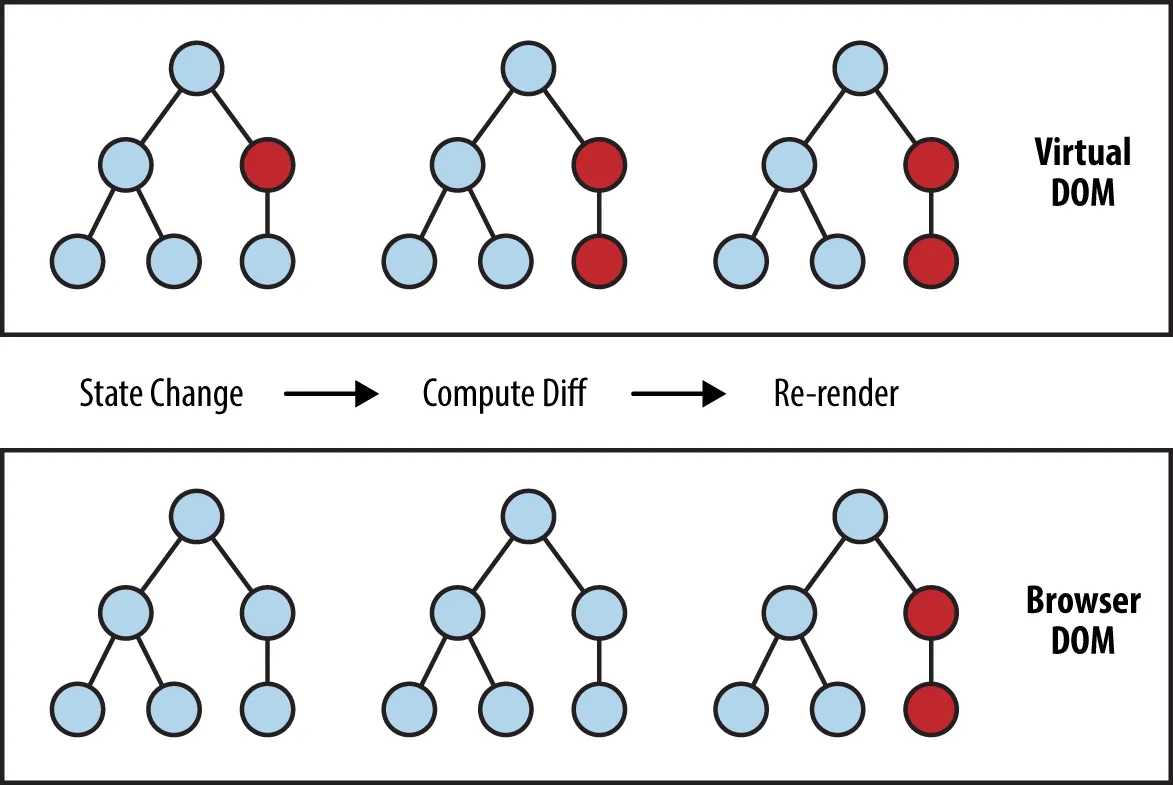
\includegraphics[width=0.8\textwidth]{images/react-dom.png}
    \caption{Schemat procesu aktualizacji Virtual DOM i rzeczywistego DOM w React. \cite{React_VDOM_Process}}
    \label{fig:react-vdom}
\end{figure}

Wraz z wprowadzeniem architektury React Fiber przebudowano wewnętrzny mechanizm odpowiedzialny za przetwarzanie aktualizacji komponentów. Fiber stanowi asynchroniczny, priorytetowy model renderowania, który umożliwia dzielenie procesu odświeżania na mniejsze części oraz nadawanie priorytetów poszczególnym aktualizacjom \cite{React_Concurrent_Docs}. Dzięki temu React może bardziej efektywnie reagować na interakcje użytkownika oraz zapewniać płynność działania nawet wtedy, gdy aplikacja wykonuje złożone operacje w tle.

Istotnym elementem architektury Reacta jest również cykl życia komponentów, który definiuje, w jakich momentach aplikacja może odwołać się do logiki zewnętrznej lub wykonać działania związane z odświeżaniem widoku. Wraz z wprowadzeniem hooków cykl życia został uproszczony i ujednolicony, co znacząco zwiększyło elastyczność zarządzania stanem oraz zachowaniami komponentów. Hooki, takie jak \texttt{useState}, \texttt{useEffect} czy \texttt{useRef}, pozwalają na precyzyjne kontrolowanie efektów ubocznych, aktualizacji stanu oraz interakcji z elementami DOM \cite{React_Lifecycle_Chart}.

Podsumowując, architektura Reacta opiera się na czytelnej strukturze komponentów, deklaratywnym opisie interfejsu oraz efektywnym modelu aktualizacji widoku opartym na Virtual DOM i mechanizmie Fiber. Rozwiązania te umożliwiają tworzenie aplikacji o wysokiej wydajności i dużej skalowalności, a jednocześnie zapewniają elastyczność programistyczną i przejrzystość kodu, co czyni React jednym z najpopularniejszych rozwiązań we współczesnym ekosystemie frontendowym \cite{Practical_Modern_JS}.
\subsection{Zarządzanie stanem w React}
Zarządzanie stanem stanowi jeden z fundamentów programowania w React, gdyż to właśnie wartości przechowywane w stanie determinują bieżący wygląd interfejsu oraz momenty jego odświeżania. Architektura Reacta opiera się na koncepcji unidirectional data flow (\textit{jednokierunkowy przepływ danych}), według której informacje są przekazywane hierarchicznie z góry do dołu drzewa komponentów. Zapewnia to wysoką przewidywalność cyklu życia aplikacji oraz ułatwia śledzenie przyczyn zmian w widoku \cite{React_Up_Running}.

Najpowszechniejszym sposobem przechowywania danych w komponentach funkcjonalnych jest wykorzystanie hooka \texttt{useState}. Pozwala on na zdefiniowanie lokalnego stanu, którego każda aktualizacja inicjuje proces ponownego renderowania komponentu. React optymalizuje ten proces, aktualizując jedynie te fragmenty rzeczywistego drzewa DOM, które wynikają bezpośrednio ze zmienionych danych \cite{React_Hooks_Intro}.

\begin{lstlisting}[language=tsx, caption={Przykład lokalnego zarządzania stanem przy użyciu hooka \texttt{useState}.}, label={lst:react-usestate}]
import { useState } from 'react';

function Counter() {
  const [value, setValue] = useState(0);

  const increment = () => {
    setValue(prev => prev + 1);
  };

  return (
    <button onClick={increment}>
      {value}
    </button>
  );
}
\end{lstlisting}
\source{Opracowanie własne}

W architekturze komponentowej kluczowe znaczenie ma mechanizm przekazywania danych poprzez props (\textit{właściwości}). Komponent nadrzędny może udostępnić fragment swojego stanu komponentom podrzędnym, które otrzymują go jako parametry wejściowe. Komunikacja w przeciwnym kierunku — od komponentu podrzędnego do nadrzędnego — realizowana jest poprzez przekazywanie callback functions (\textit{funkcje zwrotne}). W przypadku rozbudowanych struktur, gdzie dane muszą zostać przekazane przez wiele pośrednich poziomów, pojawia się wyzwanie określane jako prop drilling (\textit{przekazywanie właściwości przez wiele poziomów}), co może prowadzić do zmniejszenia czytelności kodu i utrudniać jego konserwację \cite{Learn_React_Design}.

W sytuacjach, w których logika aktualizacji stanu staje się bardziej złożona i obejmuje wiele wzajemnie powiązanych wartości, zaleca się zastosowanie hooka \texttt{useReducer}. Mechanizm ten opiera się na wzorcu zbliżonym do architektury Redux, w którym zmiana stanu następuje na podstawie akcji obsługiwanych przez funkcję reducer. Takie podejście sprzyja oddzieleniu logiki biznesowej od warstwy prezentacji oraz ułatwia testowanie kodu \cite{Learning_React_Third}.

\begin{lstlisting}[language=tsx, caption={Użycie hooka \texttt{useReducer} do obsługi złożonej logiki aktualizacji stanu.}, label={lst:react-usereducer}]
import { useReducer } from 'react';

function reducer(state, action) {
  switch (action.type) {
    case 'increment':
      return state + 1;
    case 'reset':
      return 0;
    default:
      return state;
  }
}

function Counter() {
  const [state, dispatch] = useReducer(reducer, 0);

  return (
    <div>
      <button onClick={() => dispatch({ type: 'increment' })}>
        {state}
      </button>
      <button onClick={() => dispatch({ type: 'reset' })}>
        Reset
      </button>
    </div>
  );
}
\end{lstlisting}
\source{Opracowanie własne}

W przypadku gdy stan musi być współdzielony pomiędzy wieloma komponentami, React oferuje mechanizm kontekstu (Context API). Pozwala on na przekazywanie danych pomiędzy odległymi elementami drzewa komponentów bez konieczności ręcznego przekazywania ich przez kolejne poziomy hierarchii. Mechanizm ten jest przydatny m.in. do obsługi ustawień aplikacji, motywów graficznych czy globalnych danych, jednak jego nadmierne stosowanie może prowadzić do niepotrzebnych renderów, jeśli struktura kontekstu nie została odpowiednio zaprojektowana \cite{React_Official}.

\begin{lstlisting}[language=tsx, caption={Podstawowy przykład użycia Context API do współdzielenia stanu.}, label={lst:react-context}]
import { createContext, useState } from 'react';

export const AppContext = createContext({
  value: 0,
  setValue: (v) => {}
});

function AppProvider({ children }) {
  const [value, setValue] = useState(0);

  return (
    <AppContext.Provider value={{ value, setValue }}>
      {children}
    </AppContext.Provider>
  );
}
\end{lstlisting}
\source{Opracowanie własne}

W przypadku dużych aplikacji lub projektów o skomplikowanej logice wymiany danych często stosowane są zewnętrzne biblioteki do zarządzania stanem, takie jak Redux, MobX lub Zustand. Redux opiera się na koncepcji pojedynczego źródła prawdy (store) oraz niezmienności danych, co zapewnia wysoki stopień przewidywalności i ułatwia debugowanie, lecz wymaga bardziej rozbudowanej konfiguracji. MobX z kolei stosuje podejście reaktywne, automatycznie monitorując zależności i aktualizując widok tylko tam, gdzie zaszły zmiany. Nowsze rozwiązania, takie jak Zustand, upraszczają zarządzanie stanem, wprowadzając prosty i deklaratywny interfejs oparty na hookach \cite{Design_Patterns_JS}.

Zarządzanie stanem ma bezpośredni wpływ na wydajność aplikacji React. Niewłaściwie zaprojektowana struktura stanów lub nadmierne ich współdzielenie może prowadzić do wielokrotnych i niepotrzebnych renderów komponentów, co negatywnie wpływa na płynność działania interfejsu. Z tego względu niezwykle istotne jest świadome projektowanie przepływu danych oraz dobór mechanizmów zarządzania stanem adekwatnych do skali i złożoności aplikacji. Szczegółowe techniki optymalizacji renderowania zostały omówione w kolejnym podrozdziale \cite{High_Perf_JS}.

Podsumowując, React dostarcza elastyczne mechanizmy zarządzania stanem, umożliwiające realizację zarówno prostych, jak i bardzo zaawansowanych scenariuszy. Wybór odpowiedniego podejścia zależy od wielkości i charakterystyki aplikacji, jednak świadome wykorzystanie dostępnych narzędzi ma kluczowe znaczenie dla utrzymania przejrzystości kodu oraz zapewnienia wysokiej wydajności renderowania interfejsu \cite{React_Up_Running}.

\subsection{Optymalizacja wydajności w aplikacjach React}
Wydajność renderowania jest jednym z kluczowych aspektów tworzenia aplikacji w React, szczególnie w przypadku interfejsów wymagających częstych aktualizacji stanu lub operujących na dużych zbiorach danych. Chociaż React dzięki mechanizmowi Virtual DOM ogranicza liczbę niezbędnych operacji na rzeczywistym drzewie DOM, to nadmierne i niekontrolowane renderowanie komponentów może nadal prowadzić do spadków płynności działania aplikacji. Z tego powodu React oferuje szereg narzędzi oraz wzorców umożliwiających optymalizację procesu renderowania i minimalizację liczby niepotrzebnych aktualizacji widoku \cite{High_Perf_JS}.

Jednym ze sposobów optymalizacji jest wykorzystanie funkcji \texttt{React.memo}, która umożliwia zapamiętywanie wyników renderowania komponentów funkcyjnych. Jeśli przekazywane do komponentu właściwości nie uległy zmianie, React renderuje go ponownie wyłącznie wtedy, gdy jest to konieczne. Mechanizm ten jest szczególnie skuteczny w przypadku komponentów o dużej złożoności, które w przeciwnym razie byłyby aktualizowane przy każdej zmianie stanu ich komponentów nadrzędnych \cite{Practical_Modern_JS}.

Drugim istotnym narzędziem są hooki \texttt{useMemo} oraz \texttt{useCallback}. Pierwszy z nich pozwala na zapamiętywanie wyników kosztownych obliczeń, dzięki czemu funkcja jest ponownie wykonywana tylko wtedy, gdy zmienią się wartości zależności. Z kolei \texttt{useCallback} umożliwia zapamiętanie referencji do funkcji, co zapobiega niepotrzebnemu przekazywaniu nowych instancji funkcji jako właściwości komponentów podrzędnych. Ma to szczególne znaczenie w sytuacjach, gdy komponenty podrzędne są opakowane w \texttt{React.memo} i reagują na zmiany referencji funkcji \cite{Learning_React_Third}.

\begin{lstlisting}[language=tsx, caption={Przykład optymalizacji renderowania komponentu przy użyciu \texttt{useMemo} oraz \texttt{React.memo}.}, label={lst:react-memo}]
import { memo, useMemo } from 'react';

const Result = memo(function Result({ items }) {
  const sum = useMemo(() => items.reduce((a, b) => a + b, 0), [items]);
  return <div>{sum}</div>;
});
\end{lstlisting}
\source{Opracowanie własne}

Optymalizacja może obejmować również odpowiednie zarządzanie strukturą stanu. Przechowywanie zbyt dużej liczby danych w stanie globalnym lub dzielenie się stanem pomiędzy zbyt wieloma komponentami prowadzi do nadmiarowych renderów. Z tego względu stan aplikacji powinien być możliwie jak najbardziej lokalny, a dane globalne należy wykorzystywać tylko wtedy, gdy faktycznie są współdzielone pomiędzy różnymi częściami interfejsu. Pomocne mogą być także techniki takie jak dzielenie komponentów na mniejsze elementy, aby ograniczyć zakres renderowania tylko do tych fragmentów, które faktycznie uległy zmianie \cite{Learn_React_Design}.

W aplikacjach wymagających wysokiej wydajności warto również stosować mechanizmy kolejkowania i opóźniania aktualizacji, dostępne poprzez \texttt{useTransition} lub \texttt{useDeferredValue}. Funkcje te wprowadzono w wersjach Reacta wspierających renderowanie współbieżne (Concurrent Mode \cite{Learning_React_Third}), co pozwala na priorytetyzowanie aktualizacji i zapewnia płynność interfejsu nawet w warunkach dużego obciążenia. Przykładowo, \texttt{useTransition} pozwala oznaczyć mniej priorytetowe operacje (np. odświeżenie wizualizacji algorytmu), dzięki czemu interakcje użytkownika (np. suwak prędkości) pozostają responsywne.

\begin{lstlisting}[language=tsx, caption={Wykorzystanie hooków \texttt{useTransition} i \texttt{useDeferredValue} do zarządzania priorytetami renderowania.}, label={lst:react-concurrent}]
import { useState, useTransition, useDeferredValue } from 'react';

function SortingVisualizer({ data }) {
  const [isPending, startTransition] = useTransition();
  const deferredData = useDeferredValue(data);

  const handleUpdate = (newData) => {
    startTransition(() => {
      // Lower priority operation
      setSortState(newData);
    });
  };

  return (
    <div style={{ opacity: isPending ? 0.8 : 1 }}>
      {/* Visualization based on deferred data */}
      <Bars items={deferredData} />
    </div>
  );
}
\end{lstlisting}
\source{Opracowanie własne}

Oprócz narzędzi programistycznych React udostępnia także profiler, umożliwiający analizę czasu renderowania poszczególnych komponentów. Profilowanie jest kluczowym elementem optymalizacji, ponieważ pozwala precyzyjnie ustalić, które elementy interfejsu generują nadmiarowe aktualizacje lub wykonują kosztowne operacje podczas renderowania \cite{Chrome_Runtime_Performance}.

Podsumowując, React oferuje rozbudowany zestaw narzędzi wspierających optymalizację wydajności aplikacji, obejmujący zarówno kontrolę nad procesem renderowania komponentów, jak i zarządzanie stanem oraz strukturą aplikacji. Świadome stosowanie dostępnych mechanizmów, takich jak \texttt{React.memo}, \texttt{useMemo}, \texttt{useCallback} czy funkcje wspierające renderowanie współbieżne, jest kluczowe dla tworzenia płynnych i responsywnych interfejsów, szczególnie w projektach wymagających dynamicznych i częstych aktualizacji widoku \cite{High_Perf_JS}.
\subsection{Integracja React z TypeScript}
Integracja React z TypeScript stanowi obecnie standardowe podejście do tworzenia nowoczesnych aplikacji frontendowych \cite{Learning_TS}. TypeScript, jako nadzbiór JavaScriptu wprowadzający statyczne typowanie, pozwala na wykrywanie błędów już na etapie kompilacji oraz zapewnia większą kontrolę nad strukturą danych. W połączeniu z deklaratywnym i komponentowym charakterem Reacta umożliwia to zwiększenie czytelności kodu, łatwiejsze utrzymanie projektu oraz wyższą przewidywalność działania aplikacji.

TypeScript znajduje zastosowanie zarówno w definicjach propsów komponentów, jak i podczas opisywania struktur stanu, funkcji pomocniczych, interfejsów oraz modeli danych obsługiwanych przez aplikację. Dzięki temu programista ma możliwość precyzyjnego określenia typów przekazywanych pomiędzy komponentami, co znacząco ogranicza ryzyko wystąpienia błędów wynikających z niezgodności typów. Typowanie jest szczególnie istotne w aplikacjach o dużej liczbie komponentów lub rozbudowanym systemie zarządzania stanem \cite{Effective_TS}.

Kluczowym elementem integracji Reacta z TypeScriptem jest użycie rozszerzenia TSX (TypeScript XML), które umożliwia łączenie składni TypeScriptu z deklaratywnym opisem komponentów Reacta. Pliki z rozszerzeniem \texttt{.tsx} pozwalają na stosowanie składni JSX wraz z pełnym wsparciem typów, co umożliwia definiowanie komponentów w sposób zbliżony do tradycyjnego JSX, ale z dodatkowymi możliwościami walidacji typów podczas kompilacji. TSX zapewnia również podpowiedzi składniowe (intellisense), ułatwia pracę z Integrated Development Environment (\textit{zintegrowane środowisko programistyczne}) oraz zwiększa czytelność kodu dzięki możliwości opisywania typów dla propsów, obiektów i funkcji bezpośrednio w definicji komponentu \cite{TypeScript_Official}.

TypeScript wspiera także typowanie hooków Reacta, takich jak \texttt{useState}, \texttt{useReducer}, \texttt{useRef} czy \texttt{useMemo}, co umożliwia tworzenie bardziej przewidywalnych i stabilnych struktur stanu. Przykładowo, zdefiniowanie typu przechowywanej wartości w \texttt{useState} pozwala uniknąć nieprawidłowych aktualizacji lub błędów wynikających z niezgodności typów. Z kolei w przypadku kontekstu Reacta (Context API) możliwość typowania wartości przekazywanych pomiędzy komponentami ułatwia tworzenie skalowalnych aplikacji z jednoznacznie zdefiniowanymi strukturami danych \cite{Pro_TypeScript}.

Integracja z TypeScriptem wpływa również na proces budowy i utrzymania aplikacji. Kompilator TypeScriptu umożliwia wczesne wykrywanie błędów, co skraca czas debugowania oraz zwiększa bezpieczeństwo wdrażania kolejnych zmian. W większych projektach TypeScript poprawia współpracę zespołu przez jednoznaczne definiowanie interfejsów i kontraktów pomiędzy komponentami, co ogranicza ryzyko błędnej interpretacji danych lub nieprzewidzianych zmian w strukturze aplikacji \cite{Code_Complete}.

Podsumowując, React w połączeniu z TypeScriptem stanowi wydajne i przewidywalne środowisko do tworzenia nowoczesnych aplikacji webowych. Integracja mechanizmów typowania, obsługi plików TSX oraz zaawansowanych narzędzi analizy statycznej pozwala na budowę skalowalnych i dobrze zorganizowanych projektów, w których elementy interfejsu oraz logika biznesowa są jasno zdefiniowane i łatwe do utrzymania \cite{Learning_TS}.

\section{Charakterystyka Angular}
Angular to kompleksowa platforma i framework programistyczny typu open source, rozwijany przez firmę Google, przeznaczony do budowy rozbudowanych, skalowalnych aplikacji webowych \cite{Angular_Docs}. W przeciwieństwie do Reacta, Angular oferuje pełny, zintegrowany ekosystem narzędzi, realizując podejście typu batteries-included (\textit{podejście z kompletem wbudowanych rozwiązań}), dostarczając ustandaryzowane rozwiązania dla wstrzyknięcia zależności (DI, Dependency Injection), obsługi formularzy, routingu oraz komunikacji asynchronicznej.

\subsection{Architektura komponentowa i nowoczesne mechanizmy reaktywności}
Architektura Angulara opiera się na hierarchii komponentów i ścisłej separacji logiki od widoku \cite{Angular_Development}. W przeciwieństwie do Reacta, Angular standardowo oddziela definicję szablonu (HTML), stylów kaskadowych (Cascading Style Sheets, CSS) oraz logiki (TypeScript) na poziomie plików lub odrębnych sekcji wewnątrz dekoratora komponentu.

\begin{lstlisting}[language=tsx, caption={Struktura komponentu w Angularze z wykorzystaniem dekoratora \texttt{@Component}.}, label={lst:angular-component-structure}]
@Component({
  selector: 'app-user',
  standalone: true,
  template: `
    <div class="user-profile">
      <h2>Profile: {{ username }}</h2>
      <button (click)="updateStatus()">Update</button>
    </div>
  `
})
export class UserComponent {
  username = 'John Smith';
  updateStatus() { /* logic */ }
}
\end{lstlisting}
\source{Opracowanie własne}

Współczesny Angular (od wersji 17+) został istotnie rozwinięty przez wprowadzenie signals (\textit{sygnałów}), których założenia opisano w propozycjach zmian architektonicznych \cite{Angular_Signals_RFC}. Mechanizm ten realizuje fine-grained reactivity (\textit{reaktywność o drobnej ziarnistości}), dzięki czemu framework może precyzyjnie określić, która część szablonu zależy od konkretnej wartości stanu i wymaga odświeżenia \cite{Angular_Docs}. Z punktu widzenia wydajności jest to ważna zmiana względem tradycyjnego modelu detekcji zmian opartego na \texttt{Zone.js}, który monitorował zdarzenia asynchroniczne i inicjował sprawdzanie szerokiego zakresu drzewa komponentów \cite{Angular_Development}. Signals nie zastępują automatycznie całego dotychczasowego mechanizmu, ale pozwalają znacząco zawęzić zakres reaktywności i lepiej powiązać aktualizację widoku z rzeczywistą zmianą danych. W praktyce oznacza to możliwość korzystania z nowego modelu zarówno w konfiguracjach \textit{zoneless}, jak i w standardowych aplikacjach opartych na klasycznym procesie bootstrapowania.

Istotnej zmianie uległ również model organizacji aplikacji. Przez długi czas podstawową jednostką strukturalną były moduły (\textit{NgModules}), grupujące logicznie powiązane komponenty, dyrektywy, potoki i serwisy \cite{Angular_Docs}. Rozwiązanie to wspierało zarządzanie zależnościami oraz techniki takie jak \textit{lazy loading}, jednak wiązało się z dodatkową warstwą konfiguracji. W nowszych wersjach frameworka wprowadzono \textit{Standalone Components}, które upraszczają architekturę poprzez ograniczenie konieczności definiowania modułów dla każdego elementu. Zmniejsza to ilość \textit{boilerplate code}, czyli powtarzalnego kodu konfiguracyjnego, który nie wnosi bezpośrednio logiki biznesowej, lecz zwiększa złożoność projektu.

Fundamentalnym mechanizmem wpływającym na działanie Angulara pozostaje system detekcji zmian (\textit{Change Detection}) \cite{Angular_Docs}. To on odpowiada za monitorowanie stanu aplikacji i aktualizowanie widoku po zmianach danych. Współczesne podejście, łączące klasyczny model detekcji zmian z mechanizmami sygnałowymi, pozwala ograniczyć narzut obliczeniowy i lepiej skalować aplikacje o dużej liczbie dynamicznych aktualizacji \cite{Learning_TS}.

\begin{figure}[h]
    \centering
    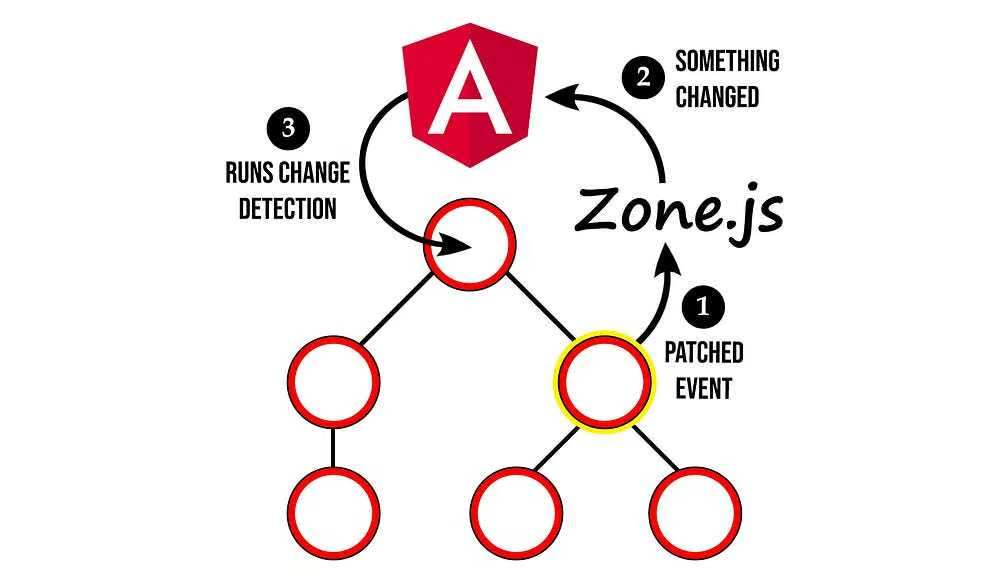
\includegraphics[width=0.85\textwidth]{images/angular-change-detection.png}
    \caption{Tradycyjny model detekcji zmian w Angularze oparty na Zone.js (sprawdzanie od góry drzewa). \cite{Angular_Change_Detection}}
    \label{fig:angular-cd}
\end{figure}

\subsection{Zarządzanie stanem w Angular}
Współczesny Angular oferuje kilka modeli zarządzania stanem, jednak w lekkich aplikacjach interaktywnych coraz większe znaczenie zyskuje podejście oparte na lokalnych sygnałach oraz wartościach pochodnych \texttt{computed()}. W takim modelu stan nie musi być utrzymywany w rozbudowanym serwisie globalnym. Zamiast tego może być przechowywany bezpośrednio w komponencie lub w niewielkiej klasie kontrolera, a widok odczytuje tylko te fragmenty danych, które są mu rzeczywiście potrzebne \cite{Angular_Docs}.

RxJS (Reactive Extensions for JavaScript) pozostaje ważną częścią ekosystemu Angulara i nadal jest szeroko stosowany przy integracjach sieciowych, pracy z obserwowalnymi strumieniami zdarzeń oraz złożonych procesach asynchronicznych \cite{RxJS_Action}. Nie oznacza to jednak, że każda aplikacja Angular musi budować logikę stanu na \texttt{Subject} i \texttt{BehaviorSubject}. W przypadku wizualizatorów algorytmów, gdzie najważniejsza jest przewidywalna lokalna aktualizacja listy elementów, model sygnałowy okazuje się prostszy i bliższy rzeczywistemu przebiegowi animacji.

\begin{lstlisting}[language=tsx, caption={Zarządzanie stanem w Angularze przy użyciu mechanizmu Sygnałów.}, label={lst:angular-signals}]
@Component({
  selector: 'app-visualizer',
  standalone: true,
  template: `<div>Value: {{ count() }}</div>`
})
export class VisualizerComponent {
  count = signal(0);
  doubleCount = computed(() => this.count() * 2);

  increment() {
    this.count.update(v => v + 1);
  }
}
\end{lstlisting}
\source{Opracowanie własne}

W dużych systemach biznesowych można oczywiście sięgnąć po bardziej rozbudowane rozwiązania, takie jak NgRx lub warstwy serwisowe oparte na RxJS. W niniejszej pracy, ze względu na niewielki zakres domeny i silne nastawienie na pomiar renderowania, bardziej zasadne było ograniczenie architektury stanu do lokalnych struktur reaktywnych oraz jawnie kontrolowanego przepływu kroków animacji.

\subsection{Optymalizacja wydajności w aplikacjach Angular}
Wydajność w Angularze zależy przede wszystkim od efektywności procesu detekcji zmian. Kluczową techniką jest strategia \texttt{OnPush} (\textit{ChangeDetectionStrategy.OnPush}), która instruuje framework, aby sprawdzał komponent tylko wtedy, gdy zmienią się referencje jego wejściowych właściwości (\texttt{@Input()}) lub zostanie wyemitowane zdarzenie. Zastosowanie \texttt{OnPush} w połączeniu z niezmiennością danych (\textit{immutability}) pozwala na drastyczne zredukowanie liczby operacji detekcji zmian, co jest krytyczne dla zachowania płynności animacji w wizualizatorze.

Inne techniki optymalizacji obejmują \cite{Angular_Docs, High_Perf_JS}:
\begin{itemize}
    \item \textbf{Kompilator Ivy:} Generuje mniejsze pakiety danych dzięki mechanizmowi \textit{tree-shaking} oraz przyspiesza proces uruchamiania aplikacji \cite{Angular_Ivy}.
    \item \textbf{TrackBy:} Podczas renderowania list, funkcja \texttt{trackBy} pozwala Angularowi zidentyfikować, które elementy DOM odpowiadają rekordom w danych \cite{Angular_Docs}, unikając niszczenia i ponownego tworzenia całego DOM-u przy każdej zmianie w tablicy.
    \item \textbf{Deferrable Views:} Nowa funkcja umożliwiająca deklaratywne opóźnianie ładowania i renderowania fragmentów szablonu do czasu, gdy np. stają się widoczne na ekranie (\textit{viewport visibility}) \cite{Angular_Docs}.
    \item \textbf{Pure Pipes:} Stosowanie czystych potoków, które są uruchamiane tylko wtedy, gdy ich wejście ulegnie zmianie, co oszczędza cykle procesora na transformacje danych \cite{Angular_Docs}.
\end{itemize}

\subsection{Angular i TypeScript – natywna integracja}
Angular to framework zbudowany "przez TypeScript i dla TypeScripta" \cite{Angular_Development, Learning_TS}. To partnerstwo zaowocowało modelem programowania, w którym cechy języka są fundamentem działania frameworka. Wszystkie kluczowe mechanizmy, komponenty, serwisy i moduły, są definiowanymi jako klasy TypeScript z dekoratorami (np. \texttt{@Component}, \texttt{@Injectable}). Dekoratory dołączają metadane do klas, informując kompilator o ich przeznaczeniu, co pozwala na wyraźne oddzielenie konfiguracji od logiki biznesowej.

Statyczne typowanie w Angularze przynosi korzyści w postaci \cite{Angular_Development, Learning_TS}:
\begin{itemize}
    \item \textbf{Type-safe Dependency Injection:} System DI wykorzystuje typy parametrów w konstruktorze do identyfikacji zależności \cite{Angular_Development}, co zapobiega błędom w czasie uruchomienia.
    \item \textbf{Strict Template Checking:} Kompilator Angulara potrafi sprawdzić poprawność typów wewnątrz szablonów HTML, co drastycznie redukuje liczbę błędów typu \textit{undefined} \cite{Angular_Docs}.
    \item \textbf{Zaawansowane narzędzia IDE (Integrated Development Environment):} Dzięki statycznej analizie kodu, deweloperzy mogą korzystać z błyskawicznej nawigacji i automatycznej refaktoryzacji nawet w bardzo rozbudowanych projektach \cite{Learning_TS}.
\end{itemize}

Podsumowując, natywna integracja z TypeScriptem sprawia, że Angular jest frameworkiem wyjątkowo stabilnym i skalowalnym, idealnym do budowy złożonych systemów wymagających wysokiej precyzji i wydajności.

\section{Podstawy algorytmów sortujących i ich wizualizacji}
Algorytmy sortowania stanowią jeden z fundamentalnych obszarów informatyki, służąc do porządkowania elementów w zbiorze według określonej relacji \cite{Cormen_Intro}. Klasyczna literatura przedmiotu definiuje szeroki wachlarz technik optymalizacji tych procesów, które do dziś stanowią bazę dla współczesnych implementacji w silnikach JavaScript \cite{Knuth_Sorting}. W kontekście niniejszej pracy pełnią one rolę generatora intensywnego obciążenia dla silników renderujących, ponieważ proces ich wykonywania wiąże się z sekwencją licznych porównań i zamian miejsc elementów zbioru.

\subsection{Klasyfikacja i charakterystyka wybranych algorytmów sortujących}
Algorytmy sortujące można klasyfikować według wielu kryteriów, z których najważniejszymi są złożoność czasowa oraz stabilność \cite{Algorithms_Unlocked}. Złożoność czasowa określa, jak czas wykonania algorytmu rośnie wraz ze wzrostem liczby elementów ($n$). Wyróżniamy złożoność optymistyczną, średnią oraz pesymistyczną, przy czym ta ostatnia jest kluczowa dla określenia granic wydajności systemu.

Kolejnym ważnym parametrem jest złożoność pamięciowa (\textit{space complexity}), określająca ilość dodatkowej pamięci potrzebnej do wykonania operacji. Algorytmy działające w miejscu (\textit{in-place}) są preferowane w środowiskach o ograniczonych zasobach, takich jak przeglądarki mobilne \cite{High_Perf_JS}. Stabilność algorytmu natomiast informuje o tym, czy zachowuje on relatywną kolejność elementów o tych samych kluczach, co może być istotne przy sortowaniu obiektów o wielu atrybutach.

W pracy wybrano reprezentatywne algorytmy o różnej charakterystyce wydajnościowej i architektonicznej:
\begin{itemize}
    \item \textbf{Sortowanie bąbelkowe (Bubble Sort):} Jeden z najprostszych algorytmów iteracyjnych o złożoności $O(n^2)$. Choć nieefektywny dla dużych zbiorów, jest idealny do demonstracji mechanizmów detekcji zmian ze względu na bardzo regularną strukturę operacji zamiany (\textit{swap}) \cite{Sedgewick_Algorithms}. W wizualizacji pozwala on na obserwację "wypływania" największych elementów na koniec tablicy, co jest czytelne dla użytkownika, ale obciążające dla renderera przez dużą liczbę drobnych aktualizacji.
    \item \textbf{Sortowanie przez wstawianie (Insertion Sort):} Algorytm o złożoności $O(n^2)$, który buduje posortowaną część tablicy, wstawiając do niej kolejne elementy. W przeciwieństwie do Bubble Sort, znacznie rzadziej wykonuje operacje zamiany miejsc, co pozwala na porównanie, jak frameworki radzą sobie z przesuwaniem większych bloków danych w strukturze DOM \cite{Mastering_JS_Arrays}.
    \item \textbf{Sortowanie szybkie (Quick Sort):} Algorytm typu "dziel i zwyciężaj" o złożoności średniej $O(n \log n)$. Wykorzystuje element osiowy (pivot) do partycjonowania tablicy. Z punktu widzenia wizualizacji jest on wyzwaniem, ponieważ operacje następują w różnych, często odległych od siebie miejscach tablicy, co wymusza na silnikach renderujących częste zmiany w rozproszonych gałęziach drzewa widoku. Jest on kluczowy do testowania wydajności przy operacjach o wysokiej dynamice \cite{Cormen_Intro}.
    \item \textbf{Sortowanie przez scalanie (Merge Sort):} Algorytm o stabilnej złożoności $O(n \log n)$, który rekurencyjnie dzieli zbiór na mniejsze części i scala je w uporządkowany sposób. Merge Sort wymaga dodatkowej pamięci ($O(n)$), co w wizualizatorze często wiąże się z koniecznością wyświetlenia "tablic pomocniczych" lub animowania procesu kopiowania danych. Pozwala to na testowanie wydajności renderowania przy dynamicznym tworzeniu i niszczeniu elementów interfejsu \cite{Knuth_Sorting}.
\end{itemize}

\begin{lstlisting}[language=tsx, caption={Szkielet asynchronicznego algorytmu sortowania (Bubble Sort) przygotowany pod wizualizację.}, label={lst:algo-skeleton}]
async function bubbleSort(array: number[], update: (arr: number[]) => void) {
  const n = array.length;
  for (let i = 0; i < n; i++) {
    for (let j = 0; j < n - i - 1; j++) {
      if (array[j] > array[j + 1]) {
        // Swap elements
        [array[j], array[j + 1]] = [array[j + 1], array[j]];

        // State update and forcing a break for the renderer
        update([...array]);
        await new Promise(resolve => setTimeout(resolve, 10));
      }
    }
  }
}
\end{lstlisting}
\source{Opracowanie własne}

\subsection{Metody wizualizacji algorytmów}
Wizualizacja algorytmów sortowania w aplikacjach webowych sprowadza się do graficznej reprezentacji elementów zbioru (najczęściej jako słupków o różnej wysokości, gdzie wysokość odpowiada wartości elementu) oraz dynamicznej aktualizacji ich wyglądu w czasie rzeczywistym.

Efektywna wizualizacja musi uwzględniać nie tylko techniczne aspekty renderowania, ale również percepcję użytkownika. Oznacza to konieczność wprowadzenia opóźnień (\textit{delays}) między krokami algorytmu, aby proces był widoczny dla ludzkiego oka, przy jednoczesnym zachowaniu płynności animacji przejść \cite{Nielsen_Usability}.

Istnieją dwie główne architektury synchronizacji logiki algorytmu z widokiem \cite{Browser_Architecture, MDN_Web_Workers}:
\begin{itemize}
    \item \textbf{Podejście oparte na migawkach (Snapshot-based):} Algorytm jest wykonywany w izolacji od warstwy widoku, a każdy jego "krok" (porównanie, zamiana) jest zapisywany jako stan tablicy w dedykowanej kolejce (historii ruchów). Po zakończeniu obliczeń, framework odtwarza historię, renderując stany jeden po drugim z określonym interwałem \cite{Browser_Architecture}. Metoda ta gwarantuje stabilność interfejsu, ale opóźnia rozpoczęcie wizualizacji do zakończenia obliczeń, co przy rekordowo dużych zbiorach może być odczuwalne.
  \item \textbf{Podejście asynchroniczne w czasie rzeczywistym (Real-time Async):} Algorytm jest wykonywany bezpośrednio w głównej nitce (lub w Web Workerze \cite{MDN_Web_Workers}), a po każdej operacji następuje asynchroniczne przerwanie (\texttt{await sleep(ms)}). Podczas tej pauzy, stan jest aktualizowany w frameworku, co wyzwala natychmiastowe renderowanie. Jest to ważny punkt odniesienia teoretycznego dla aplikacji interaktywnych, jednak nie został wykorzystany w implementacjach badawczych opisanych w niniejszej pracy.
\end{itemize}

Wizualizacja wymaga również precyzyjnego zarządzania atrybutami graficznymi \cite{Refactoring_UI}. Kluczowe jest oznaczanie kolorami \cite{Nielsen_Usability}:
Elementy aktualnie porównywane są zazwyczaj wyróżniane kontrastowym kolorem, na przykład czerwonym, co ułatwia śledzenie bieżącego przebiegu algorytmu \cite{Refactoring_UI}. Elementy zmieniające pozycję mogą dodatkowo pulsować lub przejściowo zmieniać nasycenie koloru, dzięki czemu moment zamiany staje się bardziej czytelny dla użytkownika \cite{Refactoring_UI}. Z kolei fragmenty tablicy, które algorytm uznał za ostatecznie posortowane, są zwykle oznaczane kolorem "bezpiecznym", na przykład zielonym, co wzmacnia percepcję zakończenia danego etapu przetwarzania \cite{Refactoring_UI}.

Płynność tych zmian jest determinowana przez to, jak szybko framework potrafi zidentyfikować zmienione atrybuty CSS (komponentów lub elementów DOM) i przesłać je do silnika kompozycji przeglądarki. Optymalizacja tych przejść (np. poprzez użycie \textit{CSS Transitions} lub \textit{Transforms} zamiast zmiany szerokości/pozycji \textit{top/left}) jest niezbędna dla uniknięcia zjawiska \textit{layout thrashing}.

W niniejszym badaniu zastosowano podejście oparte na migawkach, wspólne dla obu aplikacji badawczych. Umożliwia ono wyraźne rozdzielenie fazy obliczeń od fazy prezentacji oraz zapewnia większą kontrolę nad warunkami porównania Reacta i Angulara w scenariuszach obejmujących dużą liczbę aktualizacji widoku.


\chapter{Metodyka badań i implementacja aplikacji}

\section{Założenia projektowe i wymagania funkcjonalne dla wizualizatora algorytmów}
Głównym założeniem projektowym platformy badawczej było stworzenie dwóch funkcjonalnie identycznych aplikacji, które umożliwią obiektywne porównanie wydajności renderowania w frameworkach React i Angular. Wybór wizualizacji algorytmów sortowania jako przedmiotu badania wynika z faktu, że proces ten generuje ogromną liczbę operacji na modelu danych w bardzo krótkich interwałach czasowych. Z punktu widzenia inżynierii oprogramowania, jest to scenariusz silnie obciążający mechanizmy aktualizacji widoku, ponieważ wymuszają one ciągłą rewalidację drzewa komponentów. Wizualizator musi sprostać wyzwaniu płynnego wyświetlania setek operacji na sekundę przy zachowaniu wysokiej interaktywności interfejsu, co stanowi idealny poligon doświadczalny dla mechanizmów renderowania Virtual DOM (React) i reaktywności drobnoziarnistej (Angular). Istotnym aspektem było zapewnienie technologicznej równości — obie aplikacje muszą realizować dokładnie te same zadania matematyczne, korzystając z tych samych konfiguracji systemowych, co eliminuje błąd pomiarowy wynikający z różnić w implementacji logiki biznesowej.

\subsection{Wymagania funkcjonalne i scenariusze użycia}
Projektowana aplikacja musiała spełniać szereg wymagań funkcjonalnych, które zostały podzielone na wymagania niskopoziomowe (związane z obliczeniami) oraz wysokopoziomowe (związane z interakcją). Do kluczowych funkcji należą:

\begin{enumerate}
  \item \textbf{Wielowątkowość logiczna i porównywanie równoległe}: Możliwość jednoczesnego uruchomienia wielu algorytmów w niezależnych kontenerach wizualnych. Użytkownik może wybrać różne algorytmy (np. Quick Sort vs Merge Sort) i obserwować ich zachowanie na tym samym zbiorze danych wejściowych. Wymaga to od frameworków efektywnego zarządzania wieloma niezależnymi strumieniami aktualizacji stanu bez interferencji między nimi, co odpowiada scenariuszom porównawczym stosowanym w badaniach wydajności nowoczesnych frameworków frontendowych \cite{Evaluating_Frameworks}.
  \item \textbf{Determinizm algorytmów}: Każda implementacja algorytmu musi być całkowicie deterministyczna. Oznacza to, że dla danego ziarna (\textit{seed}) generatora liczb losowych oraz tej samej wielkości tablicy, zarówno wersja React, jak i Angular, muszą wygenerować identyczną sekwencję porównań i zamian. W finalnej implementacji warunek ten spełniono przez zastosowanie wspólnego, deterministycznego generatora danych wejściowych oraz jawnie przekazywanego seeda przy każdej inicjalizacji i przetasowaniu zbioru, zamiast polegać na natywnym mechanizmie \texttt{Math.random()}, którego ziarno nie jest kontrolowane przez użytkownika \cite{MDN_Math_Random}.
  \item \textbf{Dynamiczne sterowanie czasem wykonania}: System zapewnia płynną regulację prędkości animacji w czasie rzeczywistym. Programista musi mieć możliwość modyfikacji opóźnienia (\textit{delay}) między krokami w zakresie od 1 ms (maksymalne obciążenie) do 1000 ms (tryb edukacyjny). Zmiana tego parametru nie może przerywać trwającej animacji ani powodować błędów synchronizacji w asynchronicznych funkcjach sterujących, ponieważ interfejs edukacyjny powinien zachowywać tempo zgodne z ograniczeniami ludzkiej percepcji i nie tracić poczucia płynności interakcji \cite{Nielsen_Usability}.
  \item \textbf{Zarządzanie stanem początkowym danych}: Aplikacja musi umożliwiać generowanie danych o różnej charakterystyce: całkowicie losowe, już posortowane, posortowane odwrotnie oraz z dużą liczbą duplikatów. W finalnej implementacji funkcja ta została zrealizowana jako wspólny dla obu aplikacji wybór wzorca danych wejściowych w panelu sterowania dashboardu. Każdy z tych przypadków generuje inną liczbę kroków wizualizacji, co pozwala na testowanie stabilności frameworków przy skrajnie różnych obciążeniach odpowiadających klasycznym przypadkom wejściowym analizowanym w literaturze poświęconej algorytmom sortowania \cite{Cormen_Intro, Knuth_Sorting}.
\end{enumerate}

  Z punktu widzenia scenariuszy użycia oznaczało to konieczność zaprojektowania interfejsu, który jest jednocześnie demonstracyjny i eksperymentalny. Strona powitalna miała pełnić funkcję wprowadzającą i edukacyjną, pokazując ogólną ideę działania wizualizatora, natomiast dashboard badawczy musiał udostępniać wszystkie najważniejsze parametry eksperymentu: wybór algorytmu, rozmiaru danych, wzorca wejścia, prędkości animacji oraz możliwość ponownego uruchomienia przebiegu dla nowego seeda. Taki podział ról między widokami ogranicza ryzyko przeciążenia użytkownika nadmiarem kontrolek już na etapie wejścia do aplikacji, a jednocześnie zapewnia pełną sterowalność w części właściwej dla pomiarów.

  Istotne było również zachowanie konsekwencji interakcyjnej między oboma frameworkami. Użytkownik powinien wykonywać te same operacje w porównywalnej kolejności i zbliżonym koszcie poznawczym, niezależnie od tego, czy korzysta z wersji React, czy Angular. Z tego względu w obu implementacjach przyjęto analogiczny układ sterowania: wspólny panel kontroli eksperymentu, równoległe karty algorytmów, jednolity zestaw etykiet stanów oraz preview dostępne na stronie startowej. Taka zgodność nie jest wyłącznie kwestią estetyczną, lecz elementem metodologii, ponieważ zmniejsza wpływ różnic projektowych interfejsu użytkownika (User Interface, UI) na sposób korzystania z aplikacji i interpretację wyników.

\subsection{Standardy percepcji wizualnej i kodowanie kolorystyczne}
Z punktu widzenia efektywności przekazu informacji, interfejs wizualizatora wykorzystuje system kodowania kolorystycznego, który stawia dodatkowe wyzwania przed silnikiem renderującym. Każda zmiana koloru słupka w wykresie jest traktowana jako osobna operacja aktualizacji atrybutów elementu graficznego. Przyjęto następujący standard wizualny:
\begin{itemize}
    \item \textbf{Stan spoczynku}: Słupki reprezentowane są w kolorze neutralnym, zapewniającym dobrą czytelność na tle interfejsu.
    \item \textbf{Porównanie (Active Reading)}: Elementy aktualnie odczytywane przez wskaźniki algorytmu są podświetlane kontrastowym kolorem bursztynowym. Wymaga to szybkiej zmiany klas CSS lub stylów \textit{inline} przy każdym kroku iteracji.
    \item \textbf{Zamiana i modyfikacja (Write/Swap)}: Operacje fizycznej zamiany miejsc w pamięci są sygnalizowane kolorem czerwonym. Jest to moment o największym obciążeniu, ponieważ wiąże się nie tylko ze zmianą koloru, ale również z rekompozycją pozycji w drzewie DOM lub zmianą atrybutów transformacji CSS.
    \item \textbf{Elementy specjalne (Pivoting)}: W algorytmach typu "divide and conquer", elementy pełniące funkcję punktów odniesienia są wyróżniane kolorem niebieskim, co pozwala na śledzenie struktury rekurencyjnej algorytmu.
\end{itemize}

  Tak zaprojektowany system oznaczeń ma znaczenie nie tylko dydaktyczne, ale i eksperymentalne. W wizualizacjach o wysokiej częstotliwości zmian użytkownik nie analizuje każdego słupka osobno, lecz rozpoznaje wzorce kolorystyczne i ich dynamikę w czasie. Oznacza to, że stabilność semantyki kolorów staje się częścią poprawności interfejsu: jeżeli ten sam kolor w różnych miejscach oznaczałby odmienne zdarzenia, interpretacja zachowania algorytmów byłaby znacznie trudniejsza, a samo badanie mniej wiarygodne. W rezultacie identyczna legenda i identyczny zestaw stanów w obu aplikacjach pełnią rolę mechanizmu standaryzacyjnego podobnie ważnego jak wspólny seed czy wspólne algorytmy.

  Warto podkreślić, że przyjęcie prostych kolorowych bloków zamiast bardziej dekoracyjnych form prezentacji było decyzją świadomie konserwatywną. Zrezygnowano z animacji wtórnych, gradientowego kodowania stanów czy dodatkowych etykiet liczbowych na słupkach, ponieważ mogłyby one zwiększyć koszt renderowania i utrudnić rozdzielenie narzutu warstwy prezentacji od narzutu frameworka. Celem nie było stworzenie maksymalnie efektownej infografiki, lecz kontrolowanego środowiska, w którym każdy istotny sygnał wizualny odpowiada jednoznacznej zmianie stanu algorytmu.

\subsection{Wymagania techniczne i jakość kodu}
Całość projektu technicznego oparto na języku TypeScript w wersji 5.6+, co zapewnia najwyższy poziom bezpieczeństwa typologicznego. Wykorzystanie zaawansowanych konceptów języka, takich jak \textit{Generics} i \textit{Discriminated Unions}, pozwoliło na stworzenie jednolitego modelu stanu wizualizacji (\textit{Domain Model}), który jest współdzielony między frameworkami. Architektura została zaprojektowana zgodnie z zasadą \textit{Clean Architecture} — logika matematyczna algorytmów jest całkowicie odizolowana od warstwy widoku (\textit{Presentation Layer}) i wstrzykiwana jako niezależne moduły.

Pod względem technologicznym, obie aplikacje współdzielą najważniejsze założenia badawcze, choć nie są zbudowane z identycznych bibliotek pomocniczych. Wspólne pozostają: język TypeScript, stylizacja z użyciem Tailwind CSS v4, ten sam model kroku wizualizacji (\texttt{SortStep}), ten sam seeded input oraz jednakowa koncepcja renderowania słupków jako prostych elementów DOM. Równocześnie zachowano naturalne różnice ekosystemowe: wersja React korzysta z Vite i React Routera, natomiast wersja Angular z Angular CLI (Command Line Interface) oraz Angular Routera. Dzięki temu porównanie pozostaje realistyczne, a jednocześnie eliminuje jedną z najważniejszych zmiennych zakłócających, jaką byłby odmienny mechanizm wizualizacji samych słupków.

Ważnym aspektem implementacyjnym było również zapewnienie izolacji procesów obliczeniowych. Logika algorytmów została zaimplementowana w sposób całkowicie bezstanowy (\textit{stateless}), co pozwala na jej uruchamianie w różnych środowiskach bez konieczności modyfikacji kodu źródłowego. Wykorzystanie wzorca \textit{Strategy} umożliwiło dynamiczne przełączanie algorytmów w trakcie działania aplikacji, a wspólny seed gwarantuje, że wszystkie algorytmy w obu aplikacjach rozpoczynają pracę od tego samego stanu tablicy. Tego typu rygor architektoniczny jest niezbędny, aby uniknąć sytuacji, w której jeden z frameworków byłby faworyzowany przez inną sekwencję danych wejściowych lub odmienną technologię wizualizacji.

W praktyce wymagania jakościowe dotyczyły nie tylko czytelności kodu, ale także jego audytowalności badawczej. Każdy istotny element eksperymentu musiał być możliwy do wskazania i uzasadnienia na poziomie implementacji: generator danych wejściowych, kontrakt kroku wizualizacji, mechanizm sterowania czasem, zakres parametrów oraz komponent odpowiedzialny za renderowanie słupków. Taki sposób projektowania ogranicza ryzyko „ukrytych” różnic między aplikacjami i ułatwia późniejsze zestawienie fragmentów kodu z opisem metodologicznym w pracy.

Jakość kodu w projekcie była więc rozumiana jako suma kilku własności: przewidywalności, modularności, spójności między frameworkami oraz ograniczenia zbędnych warstw pośrednich. Nie chodziło o maksymalne rozbudowanie architektury, lecz o świadome utrzymanie jej na poziomie wystarczająco prostym, by można było bronić zależności między decyzją implementacyjną a obserwowanym zachowaniem systemu. Z perspektywy badawczej taka prostota nie jest wadą, lecz warunkiem koniecznym do rzetelnej interpretacji wyników.

\section{Opis implementacji aplikacji wizualizującej w React}
Aplikacja w wersji React została zaprojektowana i zrealizowana z wykorzystaniem najnowszych standardów biblioteki w wersji 19 oraz nowoczesnych narzędzi ekosystemu JavaScript, co pozwoliło na stworzenie wydajnego i elastycznego środowiska badawczego. Głównym celem implementacji było wykorzystanie modelu programowania deklaratywnego do opisania skomplikowanych i szybko zmieniających się stanów wizualnych.

\subsection{Architektura projektu i stos technologiczny}
Struktura projektu opiera się na nowoczesnym podejściu do budowania aplikacji typu Single Page Application (SPA) \cite{SPA_Definition}, gdzie kluczową rolę odgrywa wyraźna separacja logiki biznesowej od warstwy prezentacji. Wykorzystano bibliotekę React Router v7 do obsługi nawigacji, co umożliwiło płynne przejścia między stroną powitalną (\textit{Landing Page}), wprowadzającą w tematykę badań, a głównym panelem badawczym (\textit{Dashboard}), w którym odbywa się właściwa wizualizacja. Warstwa wizualna została zbudowana w oparciu o modularną bibliotekę komponentów, co zapewnia spójność interfejsu i ułatwia jego modyfikację. Centralnym punktem aplikacji jest komponent \texttt{SortingProgressChart}, który renderuje słupki bezpośrednio jako elementy DOM z dynamicznie wyliczaną wysokością i kolorem.

Wybór narzędzi deweloperskich był podyktowany chęcią uzyskania jak najwyższej wydajności nie tylko w fazie uruchomieniowej, ale i deweloperskiej. Jako system budowania wykorzystano Vite \cite{Vite_Official}, który dzięki zastosowaniu natywnych modułów ES \cite{ECMAScript_6} w trybie deweloperskim oraz silnika Rollup w trybie budowania produkcyjnego, zapewnia niemal natychystowe odświeżanie zmian. Stylizacja opiera się na najnowszej wersji Tailwind CSS v4, która wprowadza nowy silnik generowania stylów i pozwala na implementację zaawansowanych efektów wizualnych, takich jak \textit{glassmorphism} (efekt oszronionego szkła) \cite{Tailwind_Official}. Aby przyspieszyć proces tworzenia interfejsu bez utraty kontroli nad jakością kodu, włączono do projektu zestaw komponentów Shadcn/ui \cite{Shadcn_UI}. Biblioteka ta, w przeciwieństwie do tradycyjnych pakietów menedżera Node Package Manager (NPM), dostarcza kod źródłowy komponentów bezpośrednio do projektu, co pozwala na ich pełną personalizację pod kątem specyficznych wymagań wydajnościowych wizualizatora.

Dodatkowym atutem wybranego stosu jest pełna integracja ze środowiswem TypeScript \cite{TypeScript_Official}. Każdy komponent posiada ściśle zdefiniowany interfejs (\textit{props}), co eliminuje błędy związane z przekazywaniem nieprawidłowych danych w trakcie intensywnej pracy algorytmu \cite{Learning_TS}. Wykorzystanie \textit{Utility Types} pozwoliło na tworzenie elastycznych wariantów ułożenia słupków wykresu w zależności od rozdzielczości ekranu.

Architektura Reacta została podporządkowana zasadzie lokalności stanu. Oznacza to, że komponenty odpowiedzialne za prezentację nie przechowują własnej logiki sortowania, lecz otrzymują już przygotowany krok wizualizacji wraz z informacją o bieżącym stanie interakcji. Taki układ upraszcza zależności między widokami, ponieważ strona startowa, dashboard oraz karty algorytmów mogą współdzielić tę samą logikę renderowania wykresu bez duplikowania odpowiedzialności. Z perspektywy utrzymania jest to podejście korzystne, ponieważ zmiana sposobu reprezentacji kroku lub koloru stanu nie wymaga przepisywania całego przepływu aplikacji.

Warto także podkreślić znaczenie podziału na moduły domenowe i moduły interfejsowe. Wersja React nie jest zbiorem luźnych komponentów, ale uporządkowaną strukturą, w której logika sortowania, komponenty UI, hooki i trasy aplikacji mają jasno określone role. Dzięki temu analiza projektu może być prowadzona nie tylko na poziomie efektu wizualnego, ale również na poziomie organizacji kodu, co jest istotne przy późniejszej ocenie produktywności i kosztu rozwijania aplikacji.

\subsection{Podejście do zarządzania stanem i logika animacji}
Zarządzanie stanem wizualizacji zrealizowano za pomocą autorskiego hooka \texttt{useSorting}, co wpisuje się w nowoczesne wzorce projektowe biblioteki React, promujące enkapsulację logiki i współdzielenie zachowań między komponentami \cite{Learn_React_Design}. Implementacja opiera się na architekturze opartej na migawkach (\textit{Snapshot-based approach}). Zamiast modyfikować tablicę danych w czasie rzeczywistym podczas trwania animacji, algorytmy najpierw generują kompletną listę kroków (\texttt{SortStep}). Każdy taki krok definiuje unikalny stan aplikacji w danym momencie.

\begin{lstlisting}[language=tsx, caption={Struktura interfejsu opisująca krok wizualizacji w React.}, label={lst:react-step-interface}]
export type SortingProgress = {
  values: number[];
  comparing?: number[];
  swapping?: number[];
  pivot?: number | null;
  sorted?: number[];
}
\end{lstlisting}
\source{Opracowanie własne}

Hook \texttt{useSorting} pełni funkcję lokalnego kontrolera, który przechowuje tablicę wejściową, kompletną listę kroków, aktywny indeks animacji oraz bieżące parametry odtwarzania. Wykorzystanie \texttt{window.setInterval} w połączeniu z \texttt{useRef} do obsługi timera pozwala odizolować rytm animacji od samego cyklu renderowania frameworka. Istotne jest również to, że hook przyjmuje jawny seed danych wejściowych, dzięki czemu wszystkie instancje sorterów mogą pracować na identycznym zbiorze liczb i być porównywane w uczciwych warunkach.

W praktyce logika sterująca pozostała celowo prosta. Zmiana seeda, wzorca danych wejściowych lub wybór innego algorytmu powodują ponowne wygenerowanie kolejki kroków i wyzerowanie indeksu animacji, natomiast nadrzędny komponent dashboardu odpowiada za zsynchronizowane uruchamianie kilku instancji hooka równocześnie. Takie rozwiązanie nie wykorzystuje dodatkowych warstw orkiestracji ani zaawansowanych mechanizmów przerywania obliczeń, ale dzięki temu dobrze nadaje się do analizy porównawczej i ogranicza liczbę ukrytych źródeł narzutu wykonaniowego.

Ważne jest przy tym, że w modelu Reacta koszt obliczeń i koszt prezentacji zostały rozdzielone nie tylko koncepcyjnie, ale także czasowo. Najpierw następuje wygenerowanie kompletnej sekwencji stanów dla danej konfiguracji wejścia, a dopiero później kolejne kroki są odtwarzane przez prosty mechanizm inkrementacji indeksu. W rezultacie reakcja interfejsu na zmianę parametrów, takich jak rozmiar danych, wybór algorytmu czy typ wejścia, polega przede wszystkim na wymianie całej kolejki kroków, a nie na stopniowym „przepychaniu” logiki sortowania przez warstwę widoku. Taki model jest szczególnie użyteczny badawczo, ponieważ upraszcza zależność między kosztem obliczeń a kosztem renderingu.

Architektura hooka sprzyja również wielokrotnemu wykorzystaniu tej samej logiki w różnych kontekstach interfejsu. Ten sam mechanizm sterujący może obsługiwać zarówno prosty preview na stronie startowej, jak i dashboard z czterema równoległymi kartami. Z perspektywy jakości projektu ma to duże znaczenie: spójność zachowania nie wynika z ręcznego kopiowania rozwiązań między widokami, lecz z centralizacji logiki w jednym komponencie domenowym. Dzięki temu ewentualne zmiany eksperymentalne, takie jak rozszerzenie zakresu danych lub dodanie nowego wzorca wejścia, mogą być wprowadzane w sposób bardziej kontrolowany i mniej podatny na rozjazdy między ekranami aplikacji.

\subsection{Specyficzne techniki optymalizacyjne w React 19}
Aby ograniczyć koszt odświeżania wykresu przy większych zbiorach danych, w implementacji React zastosowano kilka technik optymalizacyjnych, zgodnych z modelem pracy biblioteki i jej architekturą Fiber \cite{React_Fiber_Arch}. Jednym z kluczowych mechanizmów jest wykorzystanie wyższego rzędu komponentu \texttt{React.memo} \cite{React_Official}. Zastosowano go do opakowania komponentu \texttt{SortingProgressChart}, co wymusza na Reactcie płytkie porównywanie właściwości (\textit{props}) przed podjęciem decyzji o ponownym renderowaniu.

Kolejną istotną optymalizacją jest wykorzystanie hooka \texttt{useMemo} do przygotowania zbiorów danych przed samym procesem rysowania słupków. Indeksy elementów podlegających porównaniu lub zamianie są w każdym kroku konwertowane na obiekty typu \texttt{Set} \cite{React_Official}. Wykorzystanie struktur danych typu \textit{Set} zamiast tradycyjnych tablic pozwala na uzyskanie złożoności obliczeniowej $O(1)$ przy sprawdzaniu stanu każdego z setek słupków podczas renderowania pętli wykresu.

Dodatkowo, świadomie zrezygnowano z wykorzystania bardziej zaawansowanych mechanizmów harmonogramowania, takich jak \textit{Transitions API}, aby nie zaciemniać interpretacji wyników. Celem eksperymentu było porównanie możliwie prostych, przejrzystych implementacji, w których zależność między zmianą danych wejściowych a zachowaniem interfejsu jest łatwa do prześledzenia.

Warto również zwrócić uwagę na sposób zarządzania listą kluczy (\texttt{key}) w pętlach renderujących. W wizualizatorze każdy słupek posiada stały identyfikator oparty na indeksie, dzięki czemu React może aktualizować istniejące węzły DOM bez konieczności przebudowy całej struktury wykresu. W praktyce oznacza to, że podczas kolejnych kroków sortowania modyfikowane są przede wszystkim wysokości i kolory słupków, a koszt odświeżenia interfejsu pozostaje związany głównie z aktualizacją właściwości wizualnych, a nie z tworzeniem zupełnie nowych elementów.

Całkowita separacja fazy obliczeń od fazy prezentacji ogranicza ryzyko zjawiska \textit{jank}, co jest szczególnie ważne w środowisku takim jak React, gdzie proces odświeżania Virtual DOM generuje stały narzut na procesor. W praktyce oznacza to, że przy analizie wyników należy zwracać uwagę przede wszystkim na koszt generowania kroków, liczbę odświeżeń widoku oraz wzrost kosztu stylowania i layoutu wraz ze zwiększaniem liczby słupków.

Warto również podkreślić specyficzną dla Reacta charakterystykę zarządzania pamięcią operacyjną. Regularne re-renderowanie komponentów wiąże się z tworzeniem dużej liczby krótkotrwałych obiektów w pamięci (\textit{Garbage Generation}) \cite{High_Perf_JS}. W połączeniu z podejściem opartym na migawkach i niemutowalnych kopiach tablic oznacza to, że przy większych zbiorach danych koszt pamięciowy rośnie szybko, zwłaszcza dla algorytmów kwadratowych. Z tego względu interaktywny dashboard został przygotowany jako narzędzie do kontrolowanego zwiększania obciążenia, natomiast scenariusze skrajne wymagają ostrożnego doboru rozmiaru danych do badanego algorytmu.

\section{Opis implementacji aplikacji wizualizującej w Angular}
Wersja aplikacji przygotowana w frameworku Angular została zaimplementowana na bazie aktualnego wydania ekosystemu Angular 21, co pozwoliło wykorzystać dojrzały już model komponentów \textit{standalone}, nową składnię kontroli przepływu w szablonach oraz mechanizm Sygnałów. Celem implementacji, podobnie jak w wersji React, było stworzenie funkcjonalnie równoważnego środowiska badawczego, w którym różnice wydajnościowe będą wynikały z architektury frameworka, a nie z odmiennej logiki biznesowej czy innego sposobu wizualizacji.

\subsection{Architektura projektu i stos technologiczny}
Struktura projektu Angular została zaprojektowana w sposób celowo prosty i płaski. Warstwa aplikacyjna znajduje się w katalogu \texttt{src/app} i została podzielona na kilka podstawowych obszarów odpowiedzialności: komponent główny aplikacji z \texttt{RouterOutlet}, stronę powitalną (\textit{Landing Page}), panel badawczy (\textit{Dashboard}), moduł logiki sortowania oraz dedykowany komponent odpowiedzialny za renderowanie wykresu postępu. Routing aplikacji obsługiwany jest przez \texttt{provideRouter(routes)}, a więc bez tradycyjnych modułów \texttt{NgModule}. W praktyce oznacza to, że aplikacja posiada dwa główne widoki: ekran wejściowy oraz trasę \texttt{/dashboard}, na której użytkownik obserwuje cztery algorytmy sortowania wykonywane równolegle.

Zastosowano architekturę \textit{Standalone first}, która w Angularze 21 nie jest już eksperymentem, lecz naturalnym sposobem budowania aplikacji \cite{Angular_Docs}. Każdy kluczowy widok, taki jak \texttt{DashboardComponent}, jest samodzielnym komponentem \textit{standalone}, jawnie deklarującym własne importy. Ogranicza to ilość kodu konfiguracyjnego i ułatwia analizę zależności, co ma znaczenie zarówno dla czytelności pracy inżynierskiej, jak i dla późniejszego procesu budowania pakietu produkcyjnego. Za budowanie odpowiada nowy builder \texttt{@angular/build}, konfigurowany przez Angular CLI, który dostarcza stabilny i powtarzalny proces kompilacji, zoptymalizowany pod kątem współczesnych przeglądarek.

Warstwa wizualna została zrealizowana przy użyciu Tailwind CSS v4 oraz lokalnie włączonych komponentów biblioteki Spartan/Helm. W praktyce oznacza to wykorzystanie gotowych, ale lekkich komponentów przycisków, kart, badge'y i suwaka, bez wprowadzania ciężkiego frameworka UI z własnym rozbudowanym runtime. Jest to istotne z punktu widzenia metodologii badawczej, ponieważ pozwala utrzymać porównywalny charakter obu aplikacji i ograniczyć narzut bibliotek pomocniczych. Jednocześnie wykres nie został oparty na zewnętrznej bibliotece chartingowej, lecz na własnym komponencie \texttt{SortingProgressChartComponent}, który renderuje słupki bezpośrednio jako elementy \texttt{div} stylowane dynamicznie na podstawie bieżącego kroku algorytmu. Taka decyzja upraszcza ścieżkę renderowania i pozwala lepiej obserwować rzeczywisty narzut Angulara.

W praktyce architektura Angulara została pomyślana jako odpowiednik funkcjonalny wersji React, ale realizowany idiomami właściwymi dla tego frameworka. O ile React opiera się na hookach i funkcjach komponentowych, o tyle Angular wykorzystuje komponenty standalone, klasowy model organizacji widoku oraz wyraźniej oddziela część deklaratywną szablonu od logiki sterującej. Zachowanie porównywalnego podziału odpowiedzialności przy różnych paradygmatach implementacyjnych było istotne, ponieważ umożliwia analizę nie tylko samych wyników wydajnościowych, ale również jakości organizacji kodu w dwóch odmiennych ekosystemach.

Rozwiązanie to ma również konsekwencje praktyczne dla procesu budowania aplikacji. Angular oferuje bardziej zintegrowane środowisko projektowe, w którym routing, konfiguracja buildu, organizacja komponentów i warstwa reaktywna pozostają częścią jednego spójnego stosu. W badanym projekcie pozwoliło to ograniczyć liczbę decyzji architektonicznych narzuconych programiście na starcie, a tym samym przesunąć ciężar pracy z etapu kompletowania narzędzi na etap modelowania samego problemu badawczego.

\subsection{Podejście do zarządzania stanem i logika animacji}
Zarządzanie stanem wizualizacji w aplikacji Angular oparto na klasie \texttt{SortingPlayer}, która pełni rolę lokalnego kontrolera pojedynczego algorytmu. Każdy algorytm posiada własną instancję tej klasy, przechowującą wejściową tablicę danych, aktualny indeks kroku, stan odtwarzania, opóźnienie animacji oraz kompletną listę kroków wizualizacji. W komponencie \texttt{DashboardComponent} tworzone są cztery takie instancje: dla Bubble Sort, Quick Sort, Merge Sort oraz Insertion Sort. Dashboard przechowuje również wspólny seed i wspólny wzorzec danych wejściowych, które są propagowane do wszystkich odtwarzaczy. Dzięki temu użytkownik może obserwować jednoczesne działanie kilku algorytmów na danych o tej samej skali i o tej samej charakterystyce wejścia, a każda wizualizacja jest aktualizowana niezależnie, mimo że sterowanie odbywa się z poziomu jednego panelu.

Podobnie jak w wersji React, również tutaj przyjęto architekturę opartą na migawkach (\textit{snapshot-based}). Funkcje implementujące algorytmy sortowania nie modyfikują bezpośrednio widoku, lecz generują kolejne obiekty typu \texttt{SortStep}, zawierające stan całej tablicy oraz informacje pomocnicze o elementach aktualnie porównywanych, zamienianych, pełniących rolę pivota lub już uznanych za posortowane. Dzięki temu faza obliczeń jest jednoznacznie oddzielona od fazy prezentacji, a Angular pełni funkcję odtwarzacza gotowej sekwencji stanów.

\begin{lstlisting}[language=tsx, caption={Struktura interfejsu opisująca krok wizualizacji w Angularze.}, label={lst:angular-step-interface}]
export interface SortStep {
  values: number[];
  comparing?: number[];
  swapping?: number[];
  pivot?: number | null;
  sorted?: number[];
}
\end{lstlisting}
\source{Opracowanie własne}

Istotną cechą implementacji jest to, że stan lokalny nie został rozproszony pomiędzy wiele serwisów czy strumieni RxJS, lecz utrzymany w niewielkiej liczbie sygnałów. Klasa \texttt{SortingPlayer} korzysta z \texttt{signal()} do przechowywania bieżącego indeksu kroku, parametrów prędkości i flagi odtwarzania, natomiast \texttt{computed()} wyprowadza z nich aktualny krok, pełną listę wygenerowanych kroków oraz informację o zakończeniu sortowania. Oznacza to, że Angular przelicza tylko te wartości pochodne, które faktycznie zależą od zmienionego sygnału. Tego typu model dobrze wpisuje się w charakter problemu, ponieważ logika sterująca jest lokalna, deterministyczna i nie wymaga złożonej orkiestracji zdarzeń asynchronicznych.

Sama animacja nie jest realizowana przez osobny silnik czy bibliotekę efektów, ale przez prosty mechanizm oparty na \texttt{window.setInterval}. Komponent \texttt{DashboardComponent} synchronizuje wszystkie instancje \texttt{SortingPlayer} i okresowo wywołuje metodę \texttt{next()}, przesuwając każdą wizualizację do kolejnej migawki. Regulacja prędkości odbywa się poprzez zmianę sygnału \texttt{delay}, który jest następnie propagowany do wszystkich odtwarzaczy. Takie rozwiązanie jest inżyniersko proste, ale jednocześnie dobrze nadaje się do benchmarków, ponieważ ogranicza liczbę ukrytych warstw abstrakcji i pozwala łatwo powiązać obserwowane zachowanie aplikacji z rzeczywistą liczbą aktualizacji renderingu.

Zaletą takiego modelu jest jego duża jawność. W Angularze nie ma tu potrzeby utrzymywania odrębnego globalnego store'a ani łączenia wielu źródeł reaktywności w jedną strukturę sterującą. Każdy odtwarzacz pozostaje samowystarczalną jednostką, która przechowuje konfigurację, dane wejściowe i bieżący stan wykonania, a komponent nadrzędny zajmuje się jedynie ich synchronizacją. Tego typu kompozycja dobrze wpisuje się w praktyczne atuty współczesnego Angulara: zamiast przenosić każdą decyzję do warstwy serwisowej, można budować lokalne, dobrze określone obiekty reaktywne, których zachowanie jest łatwe do prześledzenia i obrony analitycznej.

Istotne jest również to, że klasa \texttt{SortingPlayer} została przygotowana nie tylko do odtwarzania już wybranego algorytmu, ale także do rekonfiguracji podczas działania aplikacji. Zmiana wzorca danych, rozmiaru wejścia lub samego generatora kroków może zostać przeprowadzona bez naruszania ogólnej struktury dashboardu. Z perspektywy badania oznacza to większą elastyczność eksperymentu przy zachowaniu stabilnej architektury interfejsu. Użytkownik operuje na tych samych kartach i tych samych kontrolkach, natomiast pod spodem zmienia się jedynie konfiguracja sekwencji migawkowej, co ogranicza wpływ przebudowy UI na obserwowane rezultaty.

\subsection{Specyficzne techniki optymalizacyjne w Angular 21}
Najważniejszą techniką optymalizacyjną zastosowaną w projekcie jest połączenie strategii detekcji zmian \texttt{ChangeDetectionStrategy.OnPush} z mechanizmem Sygnałów. Zarówno komponent \texttt{DashboardComponent}, jak i komponent wykresu \texttt{SortingProgressChartComponent} zostały skonfigurowane w trybie \texttt{OnPush}, dzięki czemu Angular nie wykonuje zbędnych przebiegów detekcji zmian dla całego poddrzewa widoku. Aktualizacja następuje tylko wtedy, gdy zmianie ulega konkretna wartość wejściowa lub odczytywany sygnał. W praktyce oznacza to, że koszt odświeżenia interfejsu jest silniej związany z realną zmianą danych niż z samym faktem upływu czasu czy wystąpienia zdarzenia.

Drugi istotny element stanowi nowa składnia kontroli przepływu w szablonach, przede wszystkim \texttt{@for} oraz \texttt{@if}. W dashboardzie \texttt{@for} służy do renderowania listy algorytmów i ich kart statusu, natomiast w komponencie wykresu do iterowania po słupkach i legendzie. Każda pętla korzysta z jawnego mechanizmu śledzenia elementów przez \texttt{track}, na przykład po nazwie algorytmu lub indeksie słupka. Ogranicza to liczbę niepotrzebnych operacji na DOM podczas kolejnych kroków animacji i zmniejsza ryzyko przebudowy całych fragmentów widoku przy każdej zmianie tablicy wartości.

Własny komponent wykresu stanowi kolejne świadome uproszczenie o charakterze optymalizacyjnym. Zamiast korzystać z grafiki wektorowej SVG (Scalable Vector Graphics) lub zewnętrznej biblioteki wykresów, komponent wylicza za pomocą \texttt{computed()} tablicę obiektów opisujących wysokość i kolor każdego słupka. Kolor jest dobierany na podstawie bieżącego stanu: porównania, zamiany, pivota lub zakończenia sortowania. Wynik tych obliczeń jest następnie bezpośrednio odwzorowywany w szablonie jako zestaw prostych bloków CSS. Takie podejście zmniejsza liczbę warstw pośrednich między modelem danych a końcowym drzewem DOM i pozwala analizować wydajność Angulara w stosunkowo „czystej” postaci.

Warto również podkreślić, że implementacja Angulara nie wykorzystuje w tym projekcie trybu \textit{zoneless}. W konfiguracji aplikacji obecne są wyłącznie podstawowe providery odpowiedzialne za routing i globalną obsługę błędów, bez jawnego wyłączania mechanizmu Zone.js. Z punktu widzenia rzetelności opisu ma to duże znaczenie: uzyskane wyniki wydajnościowe nie wynikają z eksperymentalnego odchudzenia frameworka, lecz z połączenia współczesnych mechanizmów Angulara 21, takich jak \textit{standalone components}, \texttt{OnPush}, \texttt{@for} oraz Sygnały. Pozwala to traktować wersję Angular jako reprezentatywną dla nowoczesnej, ale nadal praktycznej implementacji produkcyjnej.

Pod względem charakterystyki pamięciowej i renderującej, aplikacja Angular została zaprojektowana tak, aby minimalizować liczbę zbędnych rekalkulacji. Obliczenia algorytmiczne są wykonywane raz dla danej tablicy wejściowej, a późniejsze odtwarzanie polega jedynie na przesuwaniu wskaźnika aktywnej migawki. Oznacza to, że w trakcie animacji nie zachodzi ponowne uruchamianie pełnej logiki sortowania przy każdym kroku, lecz wyłącznie aktualizacja odczytu już wygenerowanej struktury danych. W rezultacie aplikacja stanowi dobrą reprezentację stylu programowania promowanego przez współczesny Angular: lokalny stan, jawne zależności reaktywne, minimalny narzut warstwy prezentacji oraz ograniczenie ciężaru bibliotek zewnętrznych do niezbędnego minimum.

\section{Metody i procedury pomiarowe dla analizy wydajności}
Analiza porównawcza wydajności frameworków React i Angular wymaga zastosowania rygorystycznej i powtarzalnej metodologii pomiarowej. Celem badań jest określenie, jak każda z technologii radzi sobie z intensywnym obciążeniem wynikającym z częstych aktualizacji interfejsu użytkownika w procesie wizualizacji algorytmów. Proces ten jest szczególnie wymagający, ponieważ wymaga od silnika przeglądarki stałego balansowania między wykonywaniem skomplikowanej logiki biznesowej (algorytmy sortowania) a odświeżaniem komponentów graficznych w tempie zbliżonym do 60 klatek na sekundę.

\subsection{Środowisko testowe i konfiguracja sprzętowa}
Wszystkie pomiary wydajności zostały przeprowadzone w ściśle kontrolowanym środowisku sprzętowo-programowym, co pozwoliło na wyeliminowanie wpływu zmiennych zewnętrznych na ostateczne wyniki. Jako platformę sprzętową wykorzystano laptop wyposażony w procesor Apple M4 Pro (architektura ARMv9.4-A z 12 rdzeniami: 8 wysokowydajnych P-cores oraz 4 energooszczędne E-cores) oraz 24 GB zunifikowanej pamięci RAM LPDDR5x. Wybór tej platformy miał kluczowe znaczenie ze względu na wysoką przepustowość pamięci (do 273 GB/s), co minimalizuje opóźnienia przy renderowaniu dużej liczby elementów DOM aktualizowanych z bardzo wysoką częstotliwością. Warstwę systemową stanowił macOS Tahoe 26.2, skonfigurowany w trybie wysokiej wydajności, z wyłączonymi funkcjami oszczędzania energii oraz zawieszonymi procesami indeksowania plików (Spotlight) i automatycznych aktualizacji systemowych.

Pomiary realizowano w sposób zautomatyzowany z wykorzystaniem Playwright uruchamiającego przeglądarkę opartą na silniku Chromium w trybie bezgłowowym (\textit{headless}). Testy wykonywano sekwencyjnie, z pojedynczym workerem oraz ustalonym rozmiarem viewportu 1440$\times$900 pikseli, co ograniczało wpływ przypadkowej zmienności środowiska wykonawczego na wyniki poszczególnych przebiegów. Obie aplikacje były serwowane lokalnie jako statyczne buildy produkcyjne, dzięki czemu pomiar dotyczył zachowania gotowych artefaktów uruchomieniowych, a nie wersji deweloperskich obciążonych dodatkowymi mechanizmami diagnostycznymi.

Kluczowym elementem metodologii było testowanie wyłącznie wersji produkcyjnych aplikacji. React był budowany standardową ścieżką \texttt{react-router build} opartą o Vite, natomiast Angular komendą \texttt{ng build} wykorzystującą builder \texttt{@angular/build}. W obu przypadkach analizie podlegały artefakty produkcyjne, a nie wersje deweloperskie, co ogranicza wpływ narzutów diagnostycznych i mechanizmów typowych dla trybu development.

\subsection{Narzędzia diagnostyczne i metryki wydajnościowe}
Do zbierania danych diagnostycznych wykorzystano zautomatyzowany harness benchmarkowy oparty na Playwright oraz Chrome DevTools Protocol. Podczas każdego przebiegu aktywowany był interfejs \texttt{Performance.getMetrics}, który dostarczał niskopoziomowych metryk czasu wykonywania skryptów, rekalkulacji stylów, layoutu, pamięci oraz struktury DOM \cite{Chrome_Runtime_Performance}. Równolegle instalowano dodatkowy próbnik runtime oparty na \texttt{requestAnimationFrame} oraz \texttt{PerformanceObserver}, co pozwalało rejestrować rytm klatek i zdarzenia typu \textit{long task}. Wyniki każdego przebiegu były zapisywane do plików JSON, a następnie agregowane w celu dalszej analizy porównawczej.

W procesie analizy skoncentrowano się na sześciu grupach metryk, które najpełniej oddają charakterystykę pracy frameworków frontendowych pod dużym obciążeniem dynamicznym \cite{Web_Vitals, Chrome_Runtime_Performance}:

\begin{enumerate}
    \item \textbf{Runtime całkowity}: Całkowity czas przebiegu scenariusza, liczony od rozpoczęcia nawigacji do dashboardu do osiągnięcia stanu końcowego benchmarku. Metryka ta ujmuje zarówno etap inicjalizacji, jak i właściwe wykonanie oraz odtworzenie wizualizacji.
    \item \textbf{Czas wykonywania skryptów i zadań}: Metryki \textit{Script Duration} oraz \textit{Task Duration} opisują koszt wykonywania logiki JavaScript, mechanizmów frameworka oraz zadań obciążających główny wątek \cite{V8_Engine_Docs}. Pozwalają one ocenić, jak duży narzut obliczeniowy generuje dany model programistyczny.
    \item \textbf{Koszt aktualizacji widoku}: Metryki \textit{Layout Duration} oraz \textit{Recalculate Style Duration} pokazują koszt obliczania geometrii elementów i przetwarzania stylów CSS \cite{Browser_Architecture}. Stanowią one bezpośredni wskaźnik tego, jak silnie aplikacja obciąża drzewo DOM podczas kolejnych kroków animacji.
    \item \textbf{Jakość rytmu klatek}: Na podstawie próbkowania \texttt{requestAnimationFrame} wyznaczano przybliżony FPS, percentyl 95 czasu klatki oraz odsetek klatek przekraczających budżet 16.67 ms, odpowiadający częstotliwości 60 Hz \cite{High_Perf_JS}. Zestaw ten pozwala ocenić nie tylko średnią płynność, ale również niestabilność animacji i występowanie \textit{micro-stutteringu}.
    \item \textbf{Total Blocking Time (TBT)}: Suma okresów, w których główny wątek pozostawał zablokowany przez zadania trwające powyżej 50 ms \cite{Web_Vitals}. Metryka ta została wyznaczona na podstawie zdarzeń \textit{long task} rejestrowanych przez \texttt{PerformanceObserver}.
    \item \textbf{Zużycie pamięci i skala drzewa dokumentu}: Analiza obejmowała również zajętość sterty JavaScript (\textit{JS Heap Used Size}) oraz pomocniczo liczbę węzłów DOM i nasłuchiwaczy zdarzeń \cite{V8_Engine_Docs}. Pozwala to powiązać koszt wykonania z rozmiarem struktury renderowanej przez aplikację.
\end{enumerate}

  Dobór tych metryk nie był przypadkowy. Razem tworzą one zestaw pozwalający obserwować problem z kilku komplementarnych perspektyw: czasu całkowitego przebiegu, kosztu wykonywania logiki, kosztu kontaktu z DOM, płynności końcowego efektu wizualnego oraz stabilności pamięciowej aplikacji. Sama analiza pojedynczej wielkości, na przykład FPS albo tylko czasu wykonywania JavaScriptu, prowadziłaby do uproszczonych wniosków. Framework może bowiem osiągać akceptowalny klatkaż kosztem większego zużycia CPU lub utrzymywać niski czas skryptów przy wyższym koszcie layoutu i rekalkulacji stylów. Dopiero zestawienie kilku metryk pozwala zbliżyć się do pełniejszego obrazu zachowania aplikacji.

  W praktyce oznacza to również konieczność ostrożnej interpretacji danych. Metryki nie opisują wyłącznie frameworka jako takiego, lecz wynik współdziałania trzech warstw: logiki algorytmu, sposobu reprezentacji stanu oraz silnika przeglądarki. Z tego powodu wnioski z pomiarów muszą uwzględniać zarówno specyfikę Reacta i Angulara, jak i fakt, że badany jest konkretny typ aplikacji: wizualizator o bardzo wysokiej częstotliwości aktualizacji. Rozsądna metodologia nie polega tu więc na mechanicznym porównaniu liczb, lecz na analizie, który komponent całego łańcucha wykonania staje się dominującym źródłem kosztu w różnych scenariuszach.

\subsection{Procedura badawcza i standaryzacja testów}
Badanie zostało podzielone na dwa scenariusze referencyjne, które różniły się poziomem obciążenia obliczeniowego i intensywnością aktualizacji interfejsu. Pierwszy scenariusz, \textit{baseline-random-32}, obejmował wizualizację czterech algorytmów sortowania (Bubble Sort, Quick Sort, Merge Sort oraz Insertion Sort) dla zbioru 32 elementów o losowym rozkładzie. Drugi scenariusz, \textit{stress-duplicates-256}, wykorzystywał ten sam zestaw algorytmów, lecz dla zbioru 256 elementów zawierających liczne duplikaty. W obu przypadkach stosowano identyczny seed generatora danych oraz opóźnienie animacji ustawione na 1 ms, co pozwalało zachować pełną porównywalność przebiegów przy jednoczesnym silnym obciążeniu mechanizmów aktualizacji widoku. Chociaż dashboardy obu aplikacji oferują z poziomu interfejsu szerszy zakres konfiguracji, zautomatyzowany pipeline benchmarkowy został świadomie ograniczony do tych dwóch scenariuszy, aby zapewnić powtarzalność pomiarów i czytelność analizy porównawczej.

Procedura pomiarowa dla każdego ze scenariuszy była rygorystycznie przestrzegana i składała się z następujących etapów \cite{Chrome_Runtime_Performance}:
\begin{enumerate}
  \item \textbf{Uruchomienie buildów produkcyjnych i serwerów statycznych}: Każda seria pomiarowa była wykonywana wyłącznie na zoptymalizowanych artefaktach produkcyjnych React i Angular, serwowanych lokalnie bez narzutu trybu developerskiego.
  \item \textbf{Inicjalizacja strony i stanu benchmarkowego}: Harness Playwright otwierał dashboard z ustalonym zestawem parametrów URL (Uniform Resource Locator), aktywował zbieranie metryk przeglądarki, oczekiwał na publikację stanu gotowości \texttt{window.\_\_SORTIFY\_BENCHMARK\_\_} oraz zapisywał snapshot początkowy aplikacji.
  \item \textbf{Rejestracja przebiegu}: W trakcie działania scenariusza równolegle zbierano metryki \textit{Performance.getMetrics} z Chrome DevTools Protocol oraz próbki czasu klatek przez \texttt{requestAnimationFrame}. Dodatkowo \texttt{PerformanceObserver} rejestrował zdarzenia \textit{long task}, co pozwalało wyliczyć \textit{Total Blocking Time}.
  \item \textbf{Zakończenie i eksport danych}: Po osiągnięciu stanu końcowego benchmarku zapisywano końcowy snapshot algorytmów oraz pełny wynik do formatu JSON (JavaScript Object Notation), obejmujący parametry scenariusza, czas całkowity przebiegu, metryki runtime, pamięci, DOM i jakości renderowania.
\end{enumerate}

Wszystkie wyniki prezentowane w dalszej części pracy dla scenariuszy referencyjnych stanowią średnią arytmetyczną z 10 niezależnych pomiarów dla każdego wariantu framework--scenariusz. Dla kluczowych metryk przekrojowych, wykorzystywanych do oceny stabilności serii, obliczono również odchylenie standardowe oraz błąd standardowy. W zastosowanym pipeline'ie nie wprowadzano automatycznego odrzucania przebiegów odstających; zamiast tego stabilność serii oceniano na podstawie rozrzutu wyników pomiędzy kolejnymi uruchomieniami. Takie podejście pozwoliło na uzyskanie danych o wysokiej powtarzalności, co jest kluczowe przy wyciąganiu wniosków o subtelnych różnicach między wydajnością React i Angular.

Sama procedura została zaprojektowana tak, aby ograniczyć wpływ zjawisk jednorazowych na końcowy obraz wydajności. Jednolity sposób uruchamiania aplikacji, stałe parametry wejściowe oraz wielokrotne powtórzenia zmniejszają znaczenie przypadkowych odchyleń sprzętowo-systemowych. Dzięki temu pomiar nie sprowadza się do pojedynczego „snapshotu” wydajności, lecz ma charakter bardziej reprezentatywny dla rzeczywistego działania aplikacji w stabilnych warunkach.

Warto również zauważyć, że nawet ograniczona do dwóch scenariuszy matryca badawcza zachowuje charakter porównawczy o wyraźnie odmiennych profilach obciążenia. Scenariusz bazowy pozwala ocenić zachowanie frameworków przy umiarkowanej liczbie operacji i relatywnie małym zbiorze danych, natomiast scenariusz obciążeniowy eksponuje koszt aktualizacji widoku przy dużej liczbie elementów i wysokiej liczbie powtarzalnych operacji. Dzięki temu analiza nie sprowadza się do prostego wskazania „szybszego” frameworka, lecz umożliwia obserwację, jak oba podejścia zachowują się w warunkach lekkiego i silnego obciążenia.

\subsection{Wyzwania w standaryzacji i neutralizacja zmiennych}
Projektowanie rzetelnego badania dla dwóch tak odmiennych modeli renderowania wiąże się z wyzwaniem tzw. niedopasowania impedancyjnego (\textit{Impedance Mismatch}). Aby zapewnić sprawiedliwość benchmarku, konieczne było zagwarantowanie parzystości najważniejszych elementów wpływających na koszt odświeżania widoku. W obu wersjach aplikacji każdy słupek jest więc renderowany jako prosty element DOM o dynamicznie sterowanej wysokości i kolorze, a nie przez różne biblioteki wykresów. Standaryzacja polegała również na wymuszeniu, aby oba frameworki przetwarzały dokładnie ten sam strumień danych o krokach algorytmu, generowany dla tego samego seeda, co pozwala ocenić wewnętrzną sprawność mechanizmów aktualizacji, a nie koszt odmiennej reprezentacji graficznej.

Dodatkowo, podjęto kroki w celu neutralizacji mechanizmów specyficznych dla technologii, które mogłyby zaburzać wyniki. Zachowano natywne dla ekosystemu mechanizmy budowania i routingu, ale ujednolicono sam sposób wizualizacji, zestaw algorytmów oraz model danych wejściowych. Dzięki temu wyniki można interpretować jako porównanie dwóch dojrzałych, lecz możliwie prostych implementacji tego samego problemu badawczego.

Standaryzacja nie oznaczała jednak pełnej identyczności całych środowisk uruchomieniowych, ponieważ taka identyczność byłaby w praktyce niemożliwa i metodologicznie dyskusyjna. React i Angular różnią się nie tylko warstwą renderowania, ale również sposobem organizacji projektu, narzutem narzędziowym, charakterem pipeline'u budowania i modelem reaktywności. Zamiast próbować sztucznie wygładzić te różnice, projekt zachowuje elementy naturalne dla obu ekosystemów, a standaryzuje tylko te obszary, które bezpośrednio wpływają na uczciwość porównania: dane wejściowe, logikę algorytmów, reprezentację kroku oraz formę wykresu.

Takie podejście ma istotną zaletę interpretacyjną. Uzyskane wyniki nie opisują hipotetycznych, sztucznie zunifikowanych środowisk, lecz dwa rzeczywiste sposoby rozwiązania tego samego problemu w nowoczesnym frontendzie. Dzięki temu wnioski z badania mogą być bardziej użyteczne dla praktyków: zamiast odpowiadać na pytanie, który framework byłby szybszy po daleko idącej normalizacji całego stosu, pozwalają ocenić, jak zachowują się dwa dojrzałe podejścia inżynierskie przy zachowaniu podstawowej porównywalności eksperymentu.

\section{Kryteria oceny ilościowej i analiza artefaktów}
Poza analizą czysto wydajnościową, która skupia się na parametrach technicznych działania aplikacji, niniejsza praca podejmuje również próbę kompleksowej oceny obu technologii pod kątem ergonomii pracy i produktywności programisty. Jest to aspekt o znaczeniu strategicznym, często decydujący o długofalowym sukcesie projektu IT oraz kosztach jego utrzymania (\textit{Total Cost of Ownership}). Ocena produktywności ma charakter wielowymiarowy, ponieważ łączy twarde dane metryczne z bardziej jakościową perspektywą \textit{Developer Experience} (DX).

W ramach oceny obiektywnej (ilościowej) przeanalizowano szereg mierzalnych parametrów, które bezpośrednio przekładają się na szybkość dostarczania funkcji oraz łatwość refaktoryzacji kodu \cite{Clean_Code_JS, Refactoring_Fowler}. Kluczowym wskaźnikiem jest złożoność kodu źródłowego, mierzona nie tylko przez \textit{Source Lines of Code} (SLOC), ale przede wszystkim poprzez analizę złożoności cyklomatycznej (\textit{Cyclomatic Complexity}) oraz złożoności kognitywnej (\textit{Cognitive Complexity}) \cite{Code_Complete}. W aktualnym środowisku badawczym wykorzystano do tego celu własny analizator statyczny oparty na drzewie składni abstrakcyjnej (Abstract Syntax Tree, AST) TypeScript, który identyfikuje funkcje, liczy punkty decyzyjne oraz agreguje hotspoty złożoności na poziomie plików i funkcji.

Kolejnym badanym parametrem jest charakterystyka pakietu wynikowego (\textit{Bundle Analysis}). W analizie tej uwzględniono łączny rozmiar artefaktów produkcyjnych, wielkość największych plików JavaScript oraz sposób dystrybucji kodu w gotowym buildzie. Weryfikacji poddano również czas budowania aplikacji (\textit{Build Time}) w dwóch trybach: "zimnym" (bez cache) oraz przyrostowym, co jest kluczowym parametrem wpływającym na płynność pracy dewelopera w codziennych zadaniach. Dodatkowo, przeanalizowano liczbę zależności zewnętrznych, co pozwala oszacować skalę stosu pomocniczego towarzyszącego każdej implementacji.

W kontekście niniejszego projektu analiza ilościowa ma dodatkowy wymiar: pozwala zestawić deklarowaną prostotę architektury z jej rzeczywistym kosztem implementacyjnym. Jeżeli dana aplikacja osiąga zbliżone możliwości badawcze przy mniejszej liczbie plików, mniejszej liczbie zależności lub niższej złożoności kodu, stanowi to argument nie tylko techniczny, ale i organizacyjny. Z tego względu pomiar artefaktów końcowych nie może być traktowany jako poboczny dodatek do benchmarku wydajnościowego, lecz jako druga oś analizy, pokazująca cenę osiągnięcia określonego poziomu funkcjonalności.

Istotne jest także rozdzielenie metryk, które opisują sam projekt, od metryk opisujących wyłącznie runtime. Czas budowania, liczba zależności, rozmiar pakietu czy złożoność komponentów nie odpowiadają bezpośrednio na pytanie o FPS lub koszt renderowania, ale mają bezpośredni wpływ na codzienną pracę zespołu, szybkość iteracji oraz podatność kodu na regresje. W praktyce to właśnie połączenie tych dwóch perspektyw — wydajnościowej i artefaktowej — daje pełniejszy obraz przydatności frameworka w zadaniach podobnych do badanego wizualizatora.

\section{Kryteria oceny jakościowej i doświadczenie dewelopera}
Ocena jakościowa została oparta na doświadczeniach zebranych podczas pełnego cyklu życia projektu — od inicjalizacji, przez implementację algorytmów, aż po debugowanie i optymalizację finalną \cite{Pragmatic_Programmer}. Skupiono się na trzech fundamentalnych obszarach \cite{Clean_Code_JS, Pragmatic_Programmer}:

\begin{enumerate}
    \item \textbf{Ekosystem i standardy}: Analiza różnicy między "wymonitowanym" podejściem Angulara (gdzie framework dostarcza oficjalne rozwiązania dla rutingu, formularzy i walidacji \cite{Angular_Docs}) a zdecentralizowanym ekosystemem Reacta, który oferuje większą swobodę wyboru bibliotek, ale nakłada na dewelopera ciężar podejmowania decyzji architektonicznych i dbania o ich kompatybilność \cite{Learning_React_Third}.
    \item \textbf{Bariera wejścia i krzywa uczenia}: Porównanie wysiłku niezbędnego do opanowania zaawansowanych konceptów, takich jak \textit{Dependency Injection} i \textit{Observables} w Angularze \cite{Angular_Development}, w zestawieniu z modelem \textit{Hooks} i rygorem niezmienności (\textit{Immutability}) w React \cite{React_Up_Running}.
    \item \textbf{Głębokość integracji z TypeScript}: Przeanalizowano, jak silnie frameworki wymuszają poprawne typowanie \cite{Learning_TS}. Angular, będący od podstaw projektowany z myślą o TypeScript, oferuje silniejsze typowanie szablonów HTML, podczas gdy React bazuje na elastyczności JSX \cite{Practical_Modern_JS}, co daje inne doświadczenie w zakresie statycznej analizy kodu i wykrywania błędów na etapie pisania tekstu.
\end{enumerate}

Ostatnim badanym kryterium była jakość narzędzi diagnostycznych dedykowanych dla deweloperów. Porównano funkcjonalność rozszerzeń takich jak \textit{Angular DevTools} i \textit{React Developer Tools} w kontekście inspekcji stanu animacji w czasie rzeczywistym oraz profilowania zmian widoku. Synteza tych obserwacji pozwala uzupełnić ilościową analizę produktywności o perspektywę praktyki deweloperskiej.

Warto również zauważyć, że ocena produktywności uwzględniała paradygmat „wolności vs standardu”. W procesie tworzenia wizualizatora w React, deweloper staje przed koniecznością samodzielnego doboru bibliotek do zarządzania stanem asynchronicznym czy obsługi routingu, co przy braku odpowiedniego doświadczenia może prowadzić do powstania długu technicznego. Angular, poprzez swoje podejście „battery-included”, narzuca odgórnie sprawdzone wzorce projektowe, co skraca fazę planowania architektury, ale może być postrzegane jako ograniczające przy specyficznych, niskopoziomowych optymalizacjach. W badaniu szczególną uwagę poświęcono temu, jak te dwa podejścia wpływają na refaktoryzację kodu oraz utrzymanie spójności projektu w miarę wzrostu jego złożoności.

W praktyce taka ocena ma szczególne znaczenie właśnie w projekcie porównawczym, ponieważ obie aplikacje rozwijały się iteracyjnie. W toku prac zmieniał się zestaw algorytmów, sposób renderowania wykresu, zakres dostępnych parametrów eksperymentu oraz konfiguracja dashboardu i preview. Framework, który lepiej znosi takie modyfikacje bez rozrastania się kodu pomocniczego i bez pogarszania czytelności przepływu danych, zyskuje przewagę nie tylko organizacyjną, ale i metodologiczną. Stabilność procesu rozwoju staje się więc jednym z pośrednich wskaźników jakości narzędzia używanego do budowy eksperymentu.

W badanym projekcie produktywność nie była rozumiana wyłącznie jako szybkość napisania pierwszej działającej wersji. Znacznie ważniejsza była zdolność do utrzymania spójności implementacyjnej podczas kolejnych iteracji: wymiany algorytmu, dodania nowych wzorców danych, zwiększenia zakresu rozmiarów zbioru czy przebudowy komponentu wykresu. Tego typu zmiany są szczególnie cenne analitycznie, ponieważ pokazują, czy dany framework wspiera ewolucję projektu bez narastania trudnego do kontrolowania sprzężenia między logiką biznesową a warstwą widoku.

Ocena doświadczenia dewelopera obejmuje więc również jakość lokalnych kompromisów projektowych. Framework może przyspieszać start projektu, ale jednocześnie utrudniać niskopoziomowe strojenie wydajności, albo odwrotnie — dawać dużą swobodę optymalizacyjną kosztem większej liczby decyzji podejmowanych ręcznie. Właśnie w takich punktach ujawnia się praktyczna wartość ekosystemu, dokumentacji oraz konwencji narzucanych przez dane narzędzie. Rozdział ten ma więc stanowić pomost między czysto technicznym benchmarkiem a rzeczywistą perspektywą zespołu wytwarzającego i utrzymującego aplikację.

\chapter{Wyniki badań, analiza porównawcza i wnioski}

\section{Prezentacja aplikacji benchmarkowych}
Przed omówieniem wyników pomiarów zasadne jest krótkie przedstawienie aplikacji, na których przeprowadzano benchmarki. Obie wersje systemu, przygotowane odpowiednio w React i Angularze, zostały zaprojektowane jako funkcjonalnie równoważne środowiska badawcze. Oznacza to nie tylko wykorzystanie tych samych algorytmów i parametrów eksperymentu, ale również zachowanie zbliżonej struktury interfejsu użytkownika. Taka spójność ma znaczenie metodologiczne, ponieważ ogranicza wpływ odmiennych decyzji projektowych dotyczących UI na obserwowane różnice wydajnościowe.

W obu implementacjach wyróżniono dwa podstawowe widoki: stronę startową oraz dashboard badawczy. Strona startowa pełni funkcję informacyjną i wprowadzającą. Zawiera syntetyczny opis celu aplikacji, podstawowe informacje o wizualizacji algorytmów oraz podgląd sposobu prezentacji danych. Dzięki temu użytkownik jeszcze przed rozpoczęciem eksperymentu może zrozumieć logikę działania narzędzia, znaczenie kodowania kolorystycznego oraz ogólny charakter porównywanych algorytmów. Widok ten porządkuje kontekst badania i pełni rolę warstwy objaśniającej, a nie właściwego środowiska pomiarowego.

Zasadnicza część eksperymentu realizowana jest w dashboardzie badawczym. Widok ten koncentruje wszystkie elementy sterujące przebiegiem testu, takie jak uruchamianie i zatrzymywanie animacji, wybór rozmiaru danych, charakterystyki wejścia oraz tempa odtwarzania. Najistotniejszą część dashboardu stanowi zestaw czterech równoległych kart prezentujących przebieg działania poszczególnych algorytmów na tym samym zbiorze wejściowym. Takie rozwiązanie pozwala obserwować różnice w dynamice sortowania w sposób synchroniczny i porównywalny, a jednocześnie zapewnia jednakowe warunki interakcji w obu frameworkach. Z perspektywy badawczej oznacza to, że porównanie dotyczy przede wszystkim zachowania mechanizmów renderowania i aktualizacji widoku, a nie różnic wynikających z odmiennej organizacji samego interfejsu.

\clearpage
\begin{landscape}
\thispagestyle{plain}
\captionsetup{hypcap=false}
\begin{center}
  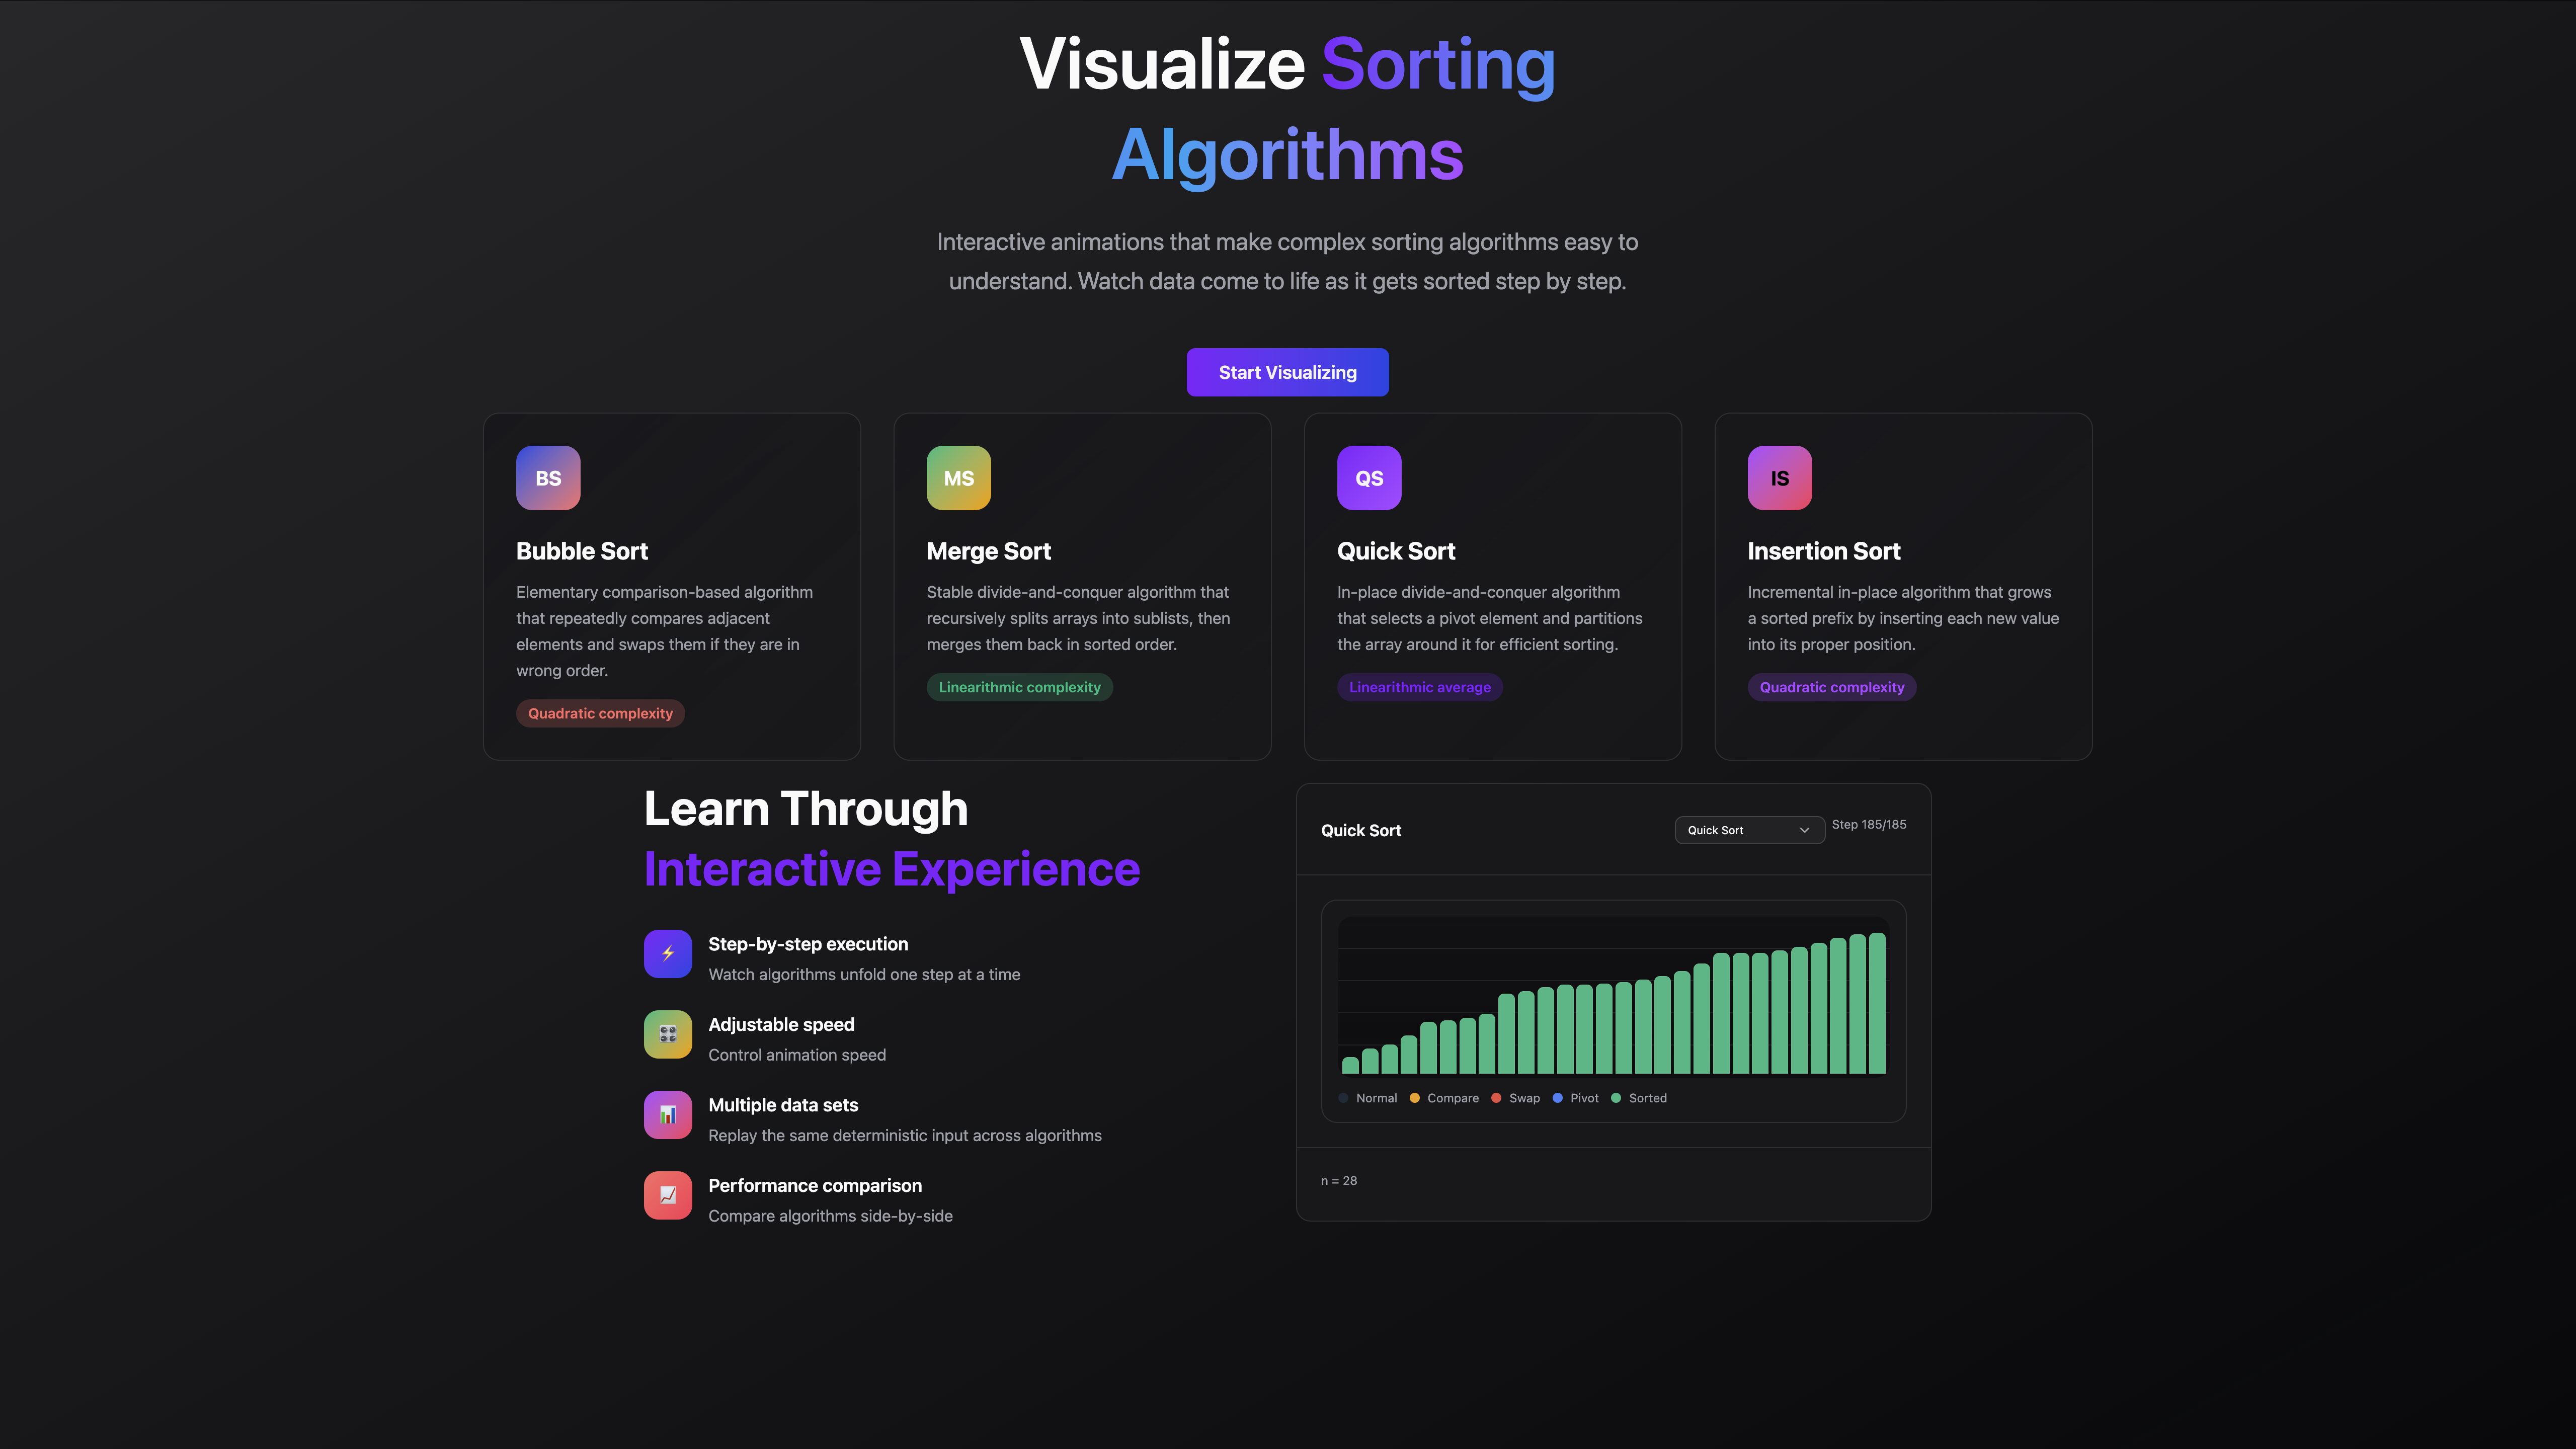
\includegraphics[width=\linewidth,height=0.82\textheight,keepaspectratio]{images/react-landing.png}
  \captionof{figure}{Strona startowa aplikacji benchmarkowej zaimplementowanej w React.}
  \label{fig:react-landing}
  \source{Opracowanie własne}
\end{center}
\end{landscape}

\clearpage
\begin{landscape}
\thispagestyle{plain}
\captionsetup{hypcap=false}
\begin{center}
  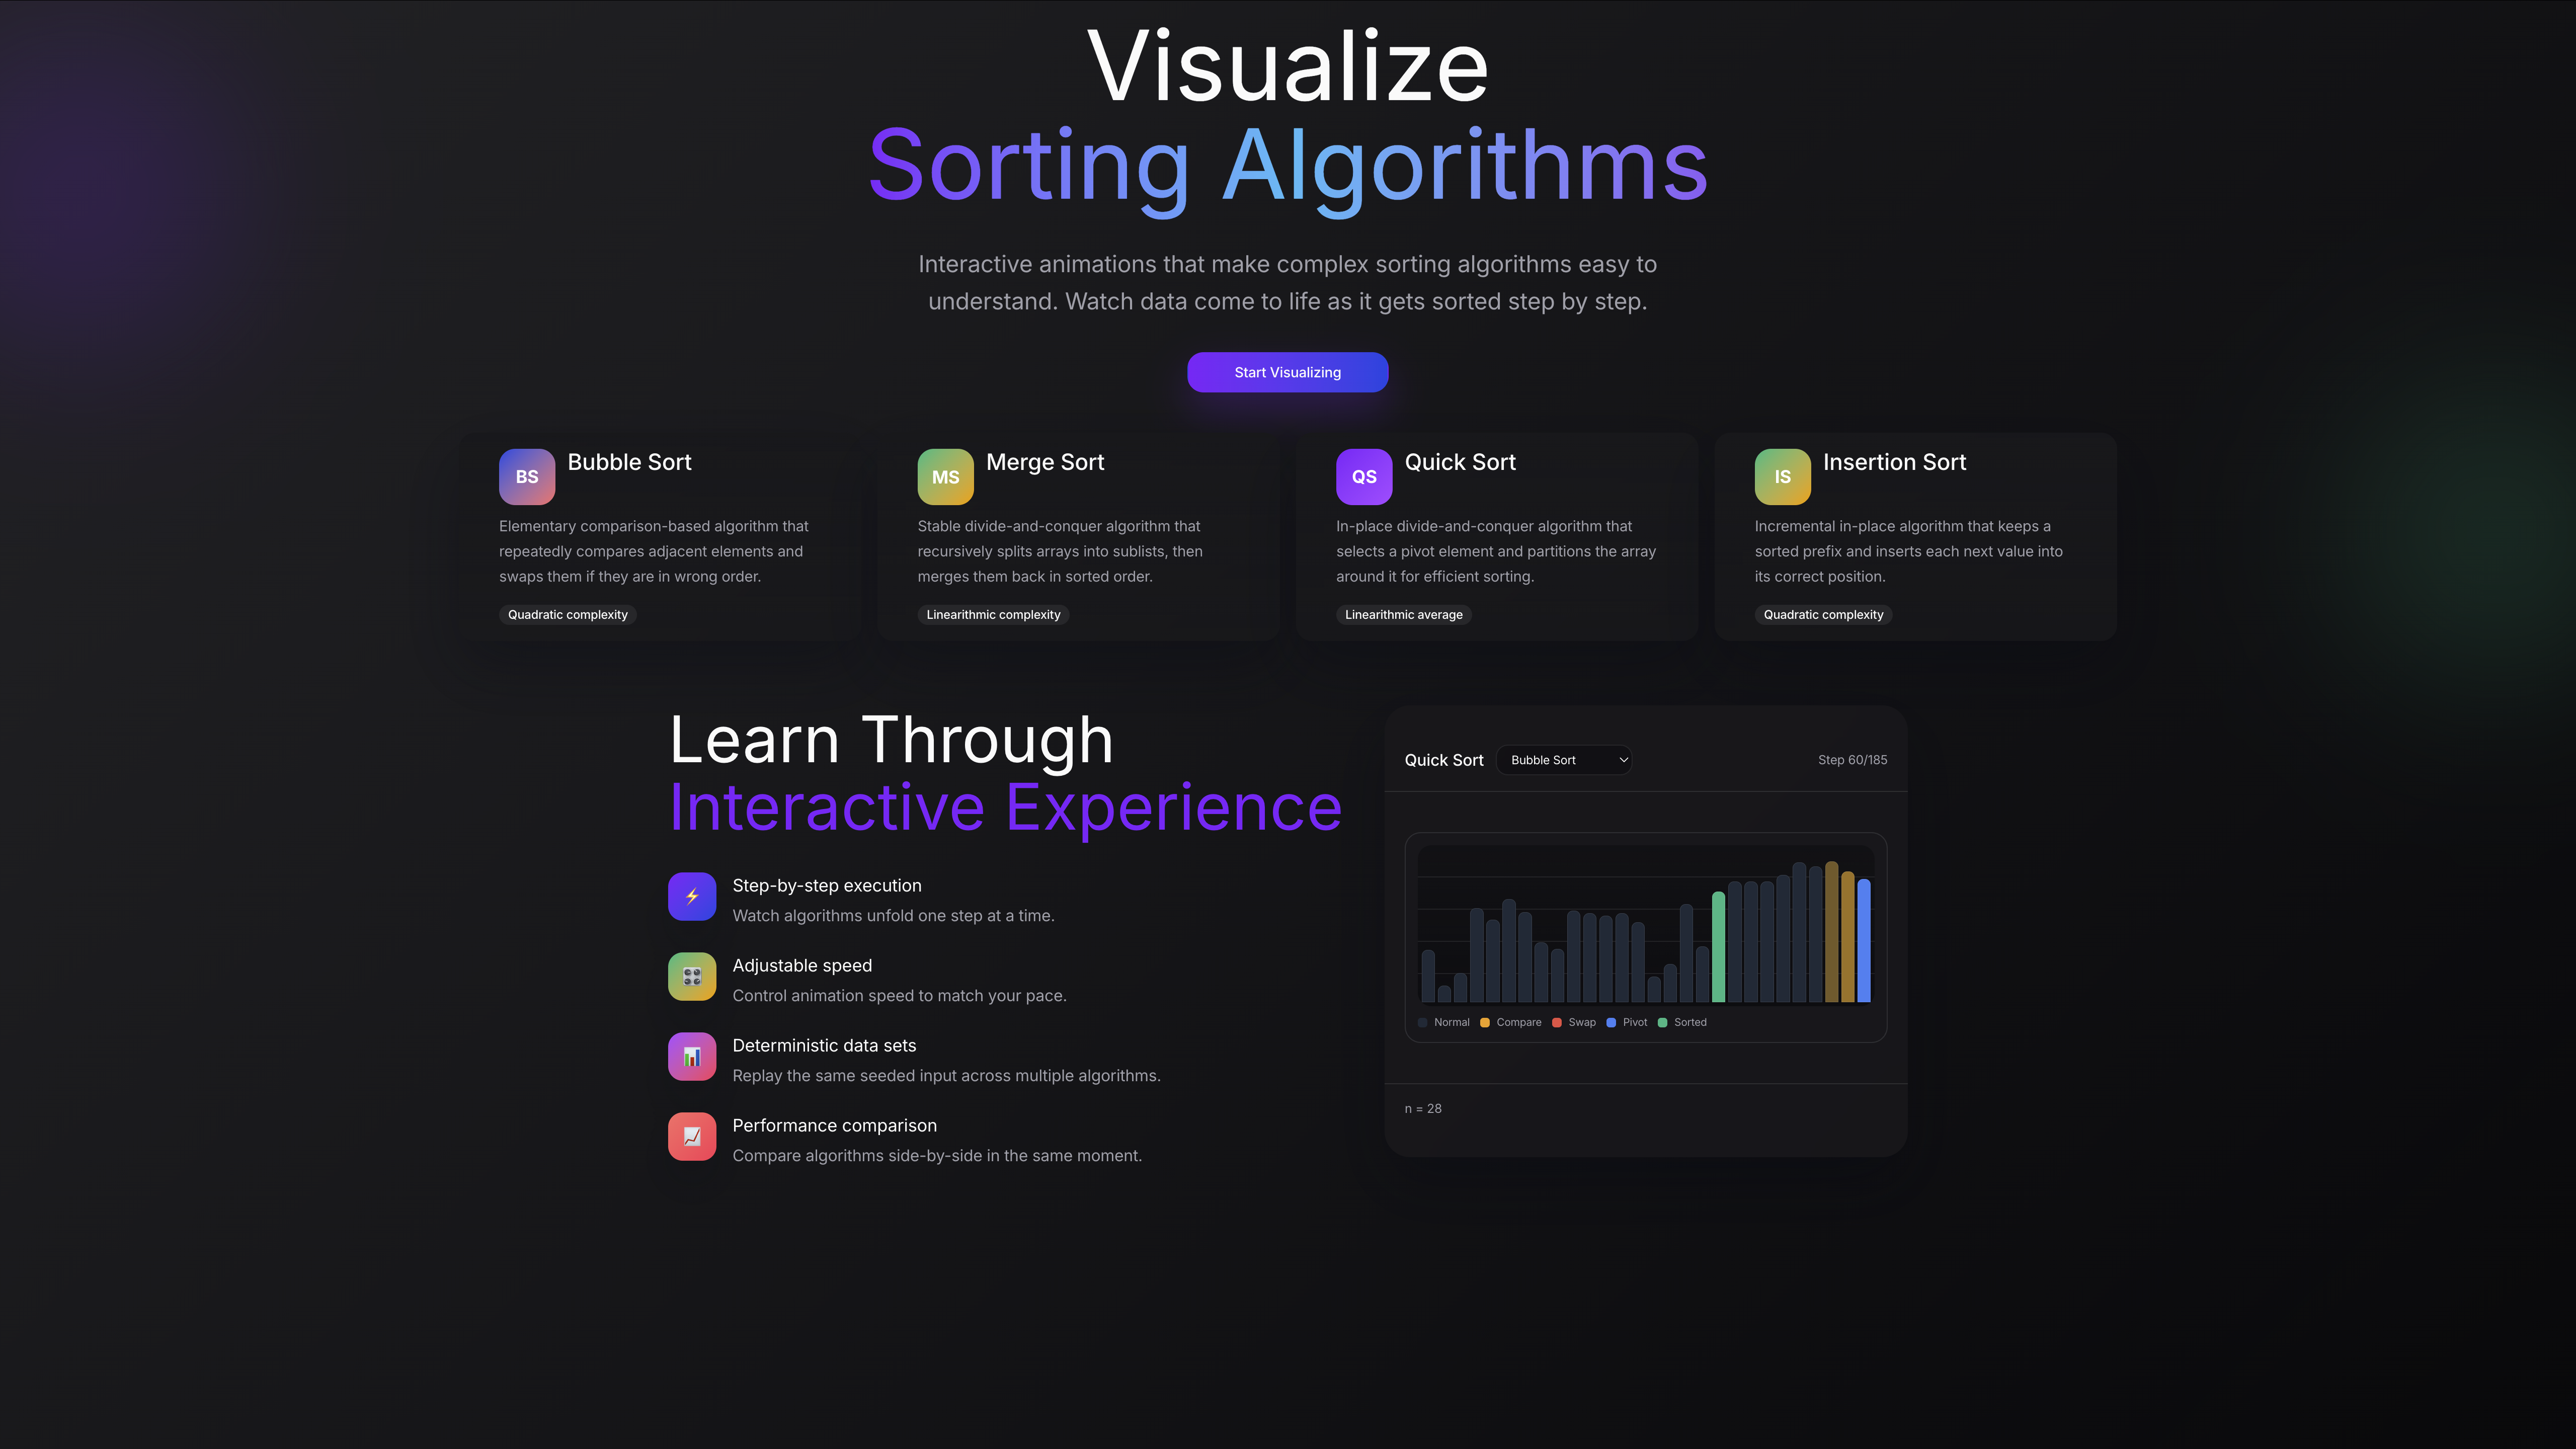
\includegraphics[width=\linewidth,height=0.82\textheight,keepaspectratio]{images/angular-landing.png}
  \captionof{figure}{Strona startowa aplikacji benchmarkowej zaimplementowanej w Angularze.}
  \label{fig:angular-landing}
  \source{Opracowanie własne}
\end{center}
\end{landscape}

\clearpage
\begin{landscape}
\thispagestyle{plain}
\captionsetup{hypcap=false}
\begin{center}
  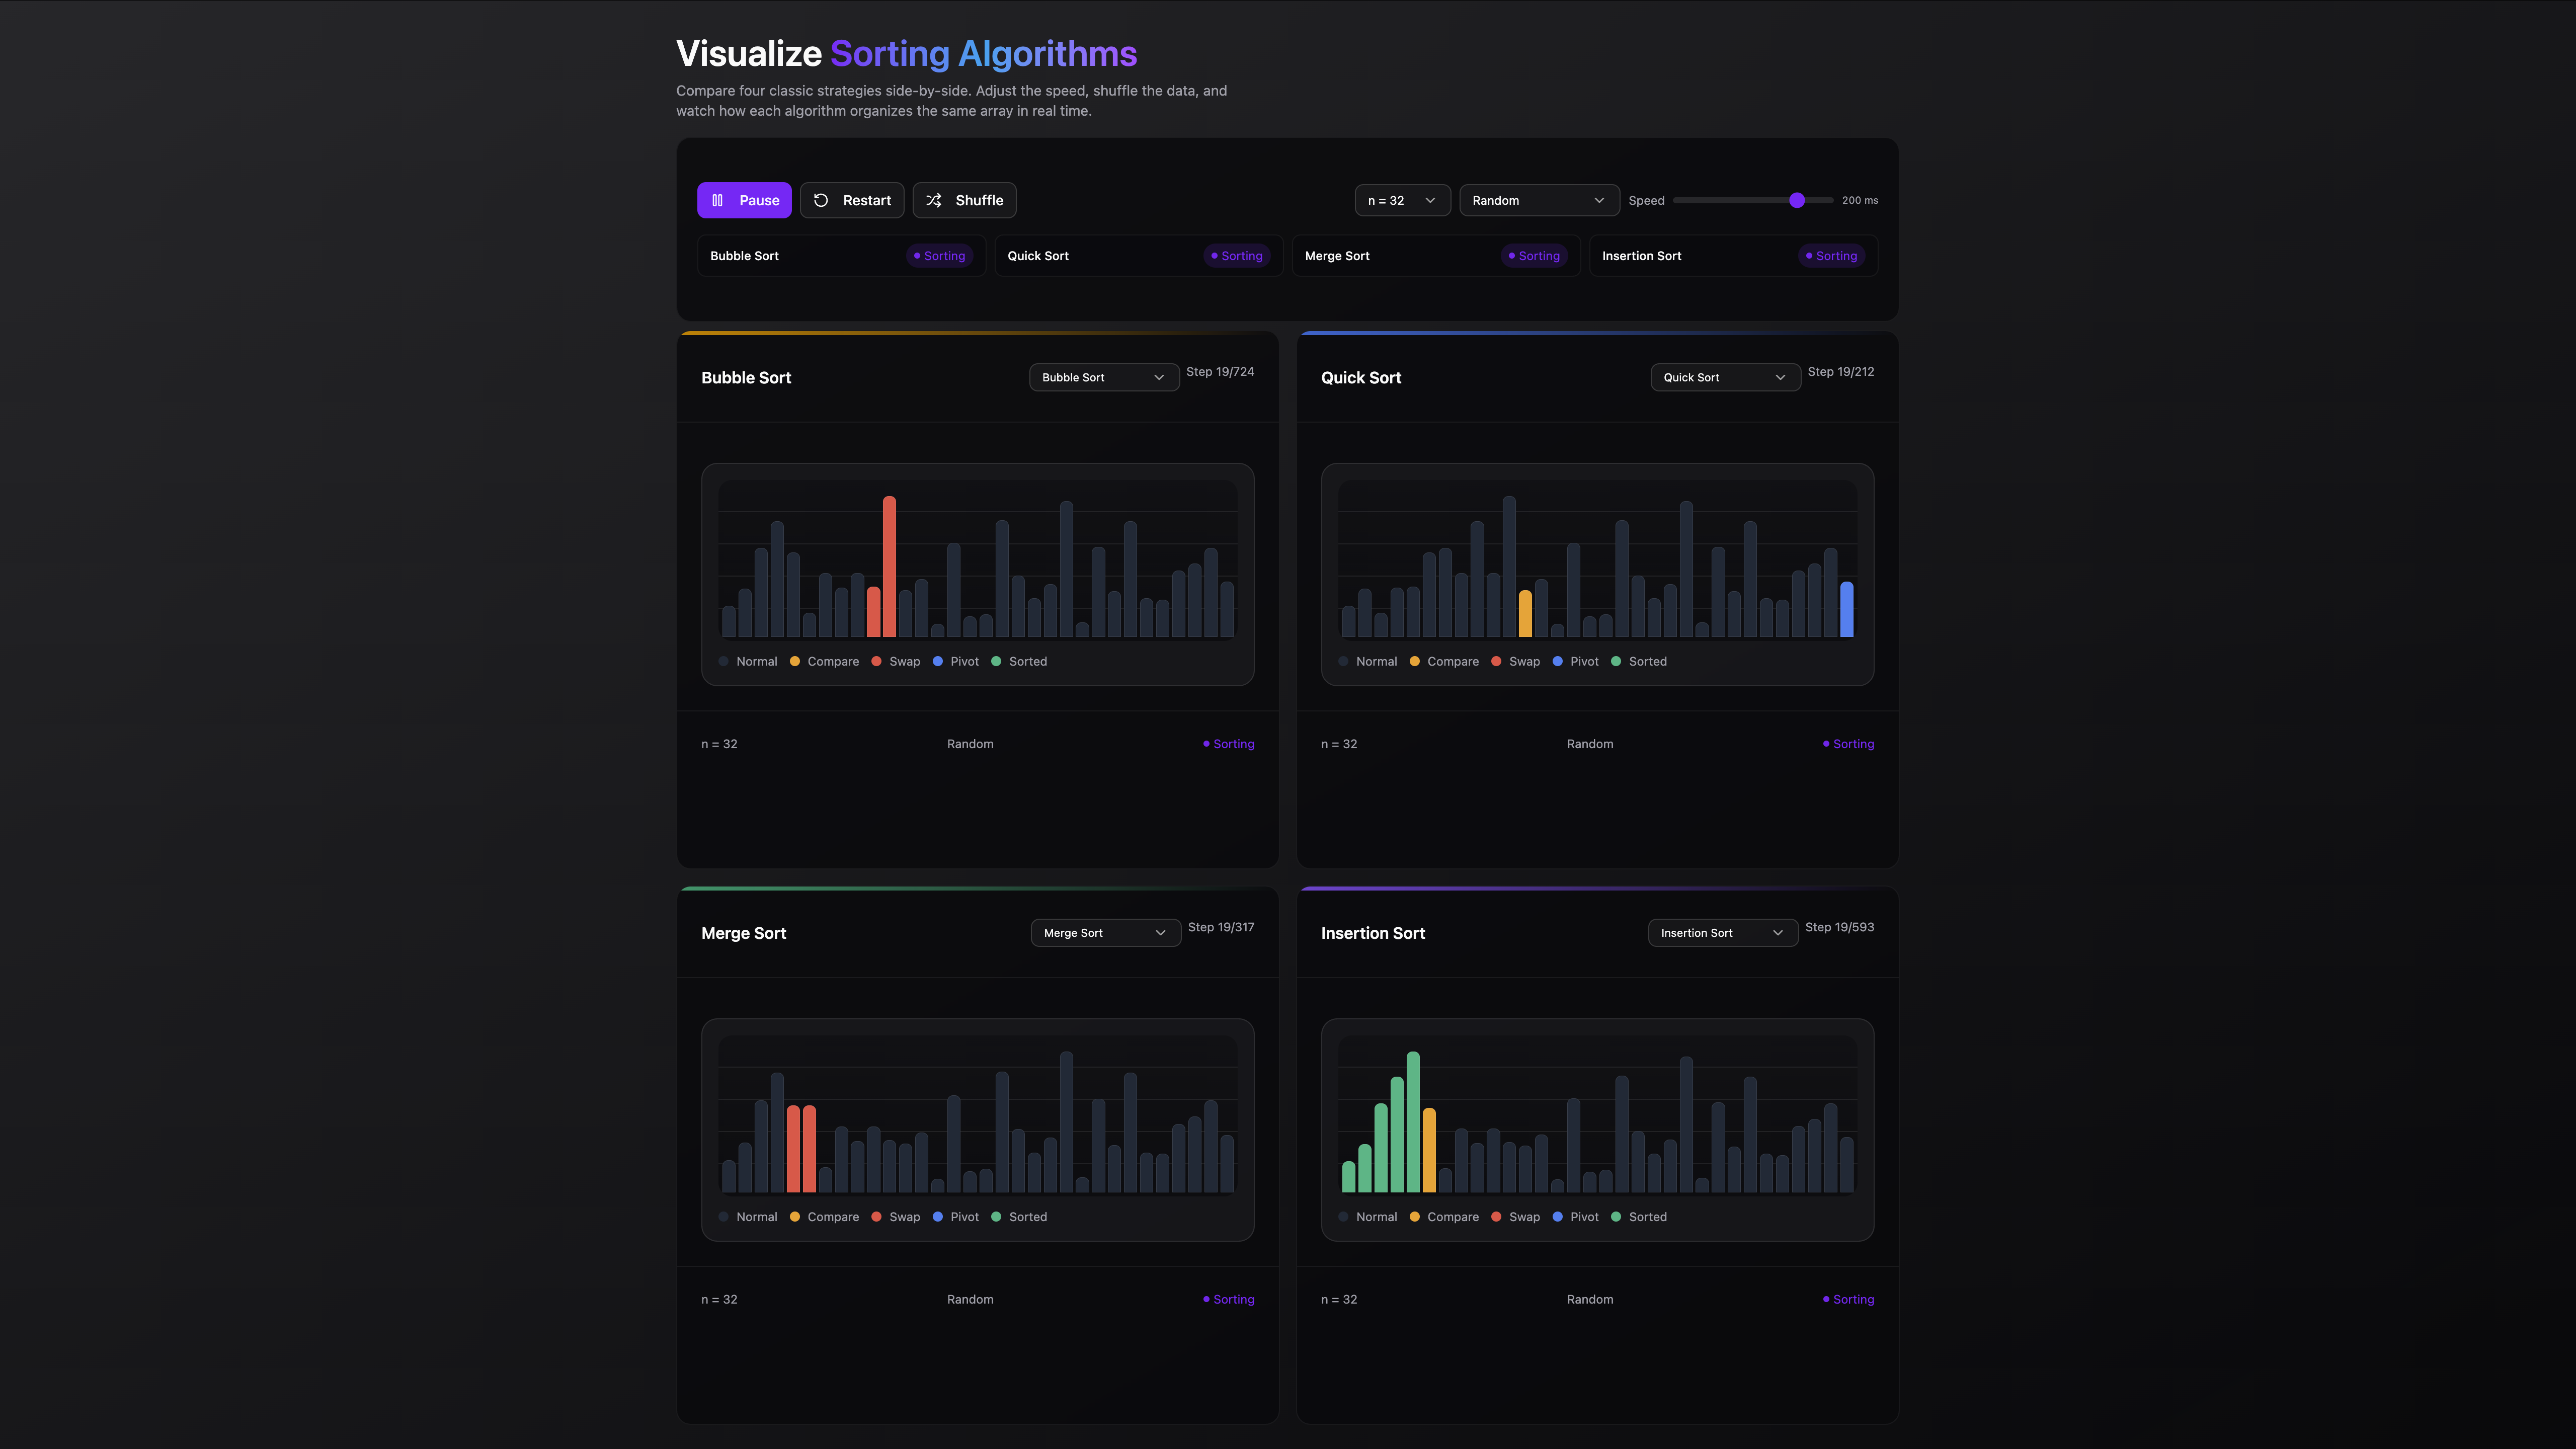
\includegraphics[width=\linewidth,height=0.82\textheight,keepaspectratio]{images/react-home.png}
  \captionof{figure}{Dashboard badawczy aplikacji benchmarkowej w React z czterema równoległymi wizualizacjami.}
  \label{fig:react-dashboard}
  \source{Opracowanie własne}
\end{center}
\end{landscape}

\clearpage
\begin{landscape}
\thispagestyle{plain}
\captionsetup{hypcap=false}
\begin{center}
  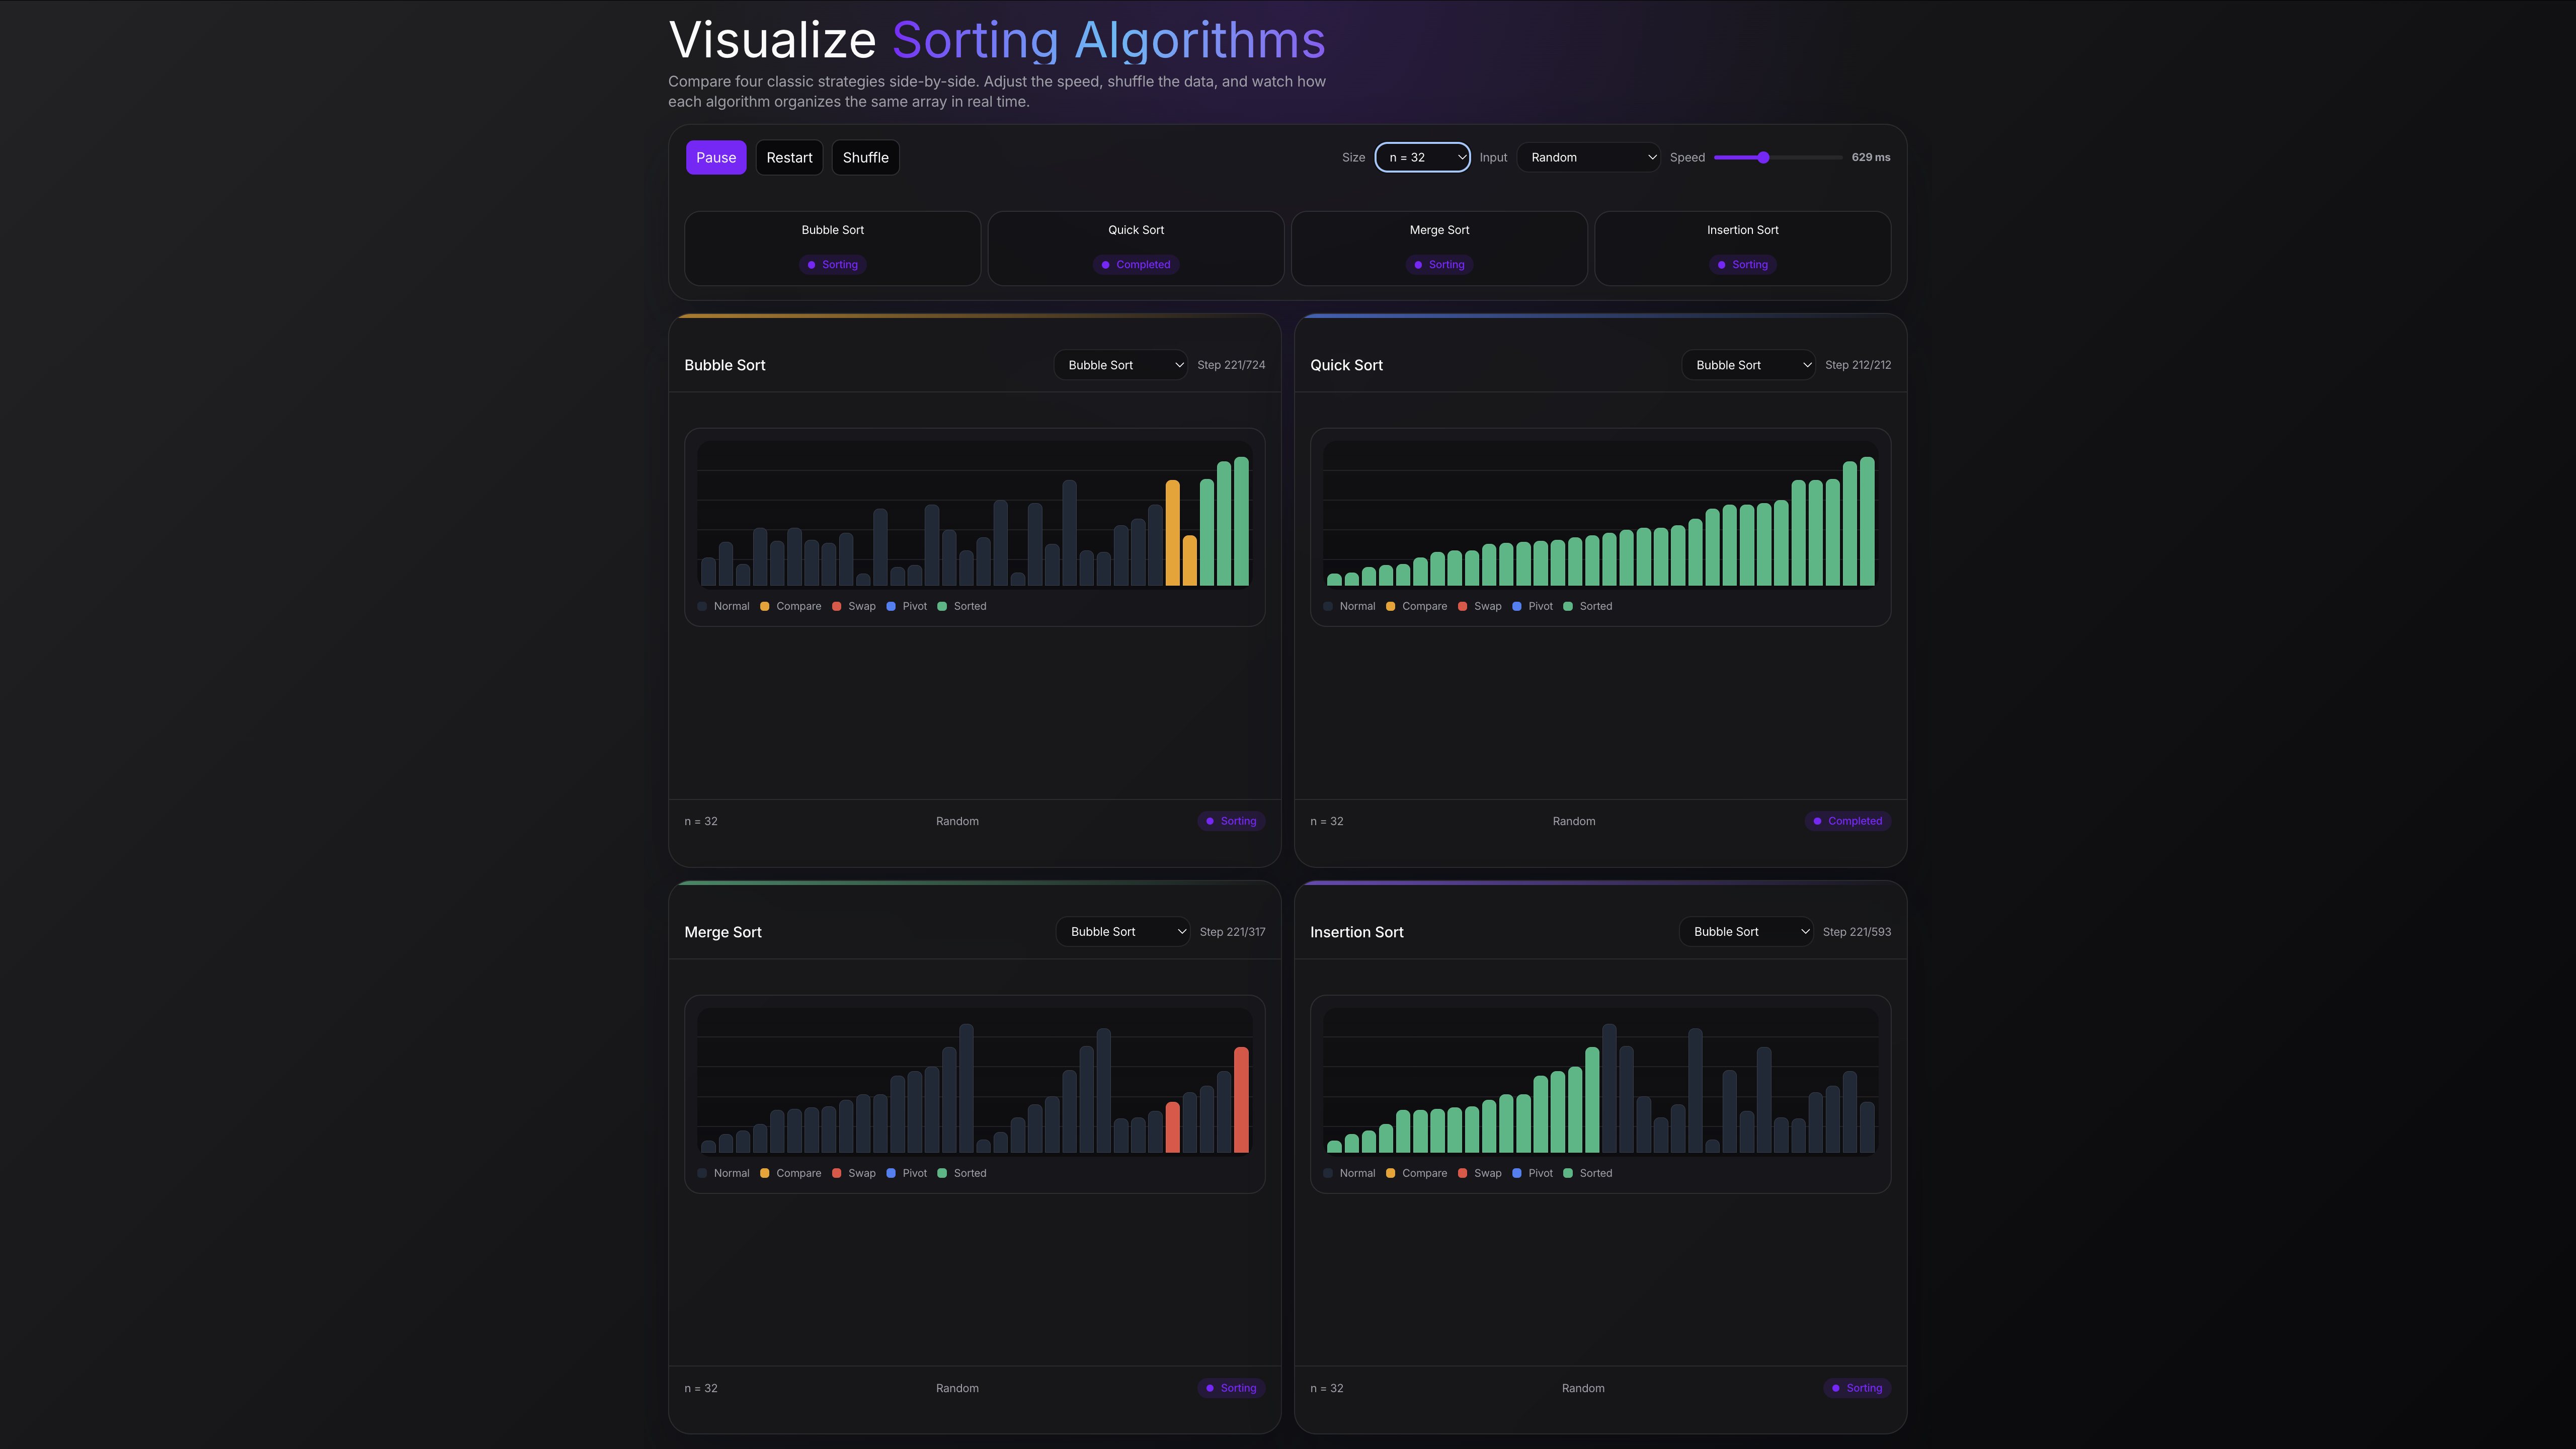
\includegraphics[width=\linewidth,height=0.82\textheight,keepaspectratio]{images/angular-home.png}
  \captionof{figure}{Dashboard badawczy aplikacji benchmarkowej w Angularze z czterema równoległymi wizualizacjami.}
  \label{fig:angular-dashboard}
  \source{Opracowanie własne}
\end{center}
\end{landscape}

\section{Prezentacja wyników pomiarów wydajności renderowania}
W niniejszym rozdziale przedstawiono wyniki uzyskane z aktualnej wersji zautomatyzowanego środowiska benchmarkowego przygotowanego dla obu aplikacji. Analizie poddano dwa scenariusze referencyjne: scenariusz bazowy \textit{baseline-random-32}, w którym równolegle wizualizowano cztery algorytmy dla 32 elementów danych losowych, oraz scenariusz obciążeniowy \textit{stress-duplicates-256}, w którym ten sam zestaw algorytmów pracował na 256 elementach z dużą liczbą duplikatów przy opóźnieniu animacji ustawionym na 1 ms. Oba przebiegi realizowano na produkcyjnych buildach aplikacji, a zbieranie danych odbywało się automatycznie z wykorzystaniem Playwright, Chrome DevTools Protocol oraz dodatkowego próbnika runtime opartego na \texttt{requestAnimationFrame} i \texttt{PerformanceObserver}, co pozwoliło zarejestrować również rytm klatek i metrykę \textit{Total Blocking Time}. Wszystkie wartości w tabelach \ref{tab:baseline-results} i \ref{tab:stress-results} są średnimi z 10 niezależnych przebiegów, a ich stabilność opisano dodatkowo w Tabeli \ref{tab:statistical-stability}.

Z perspektywy interpretacyjnej istotne jest to, że testy uruchamiają cztery wizualizacje równolegle. Oznacza to, że całkowity czas scenariusza jest w praktyce determinowany przez najdłużej wykonujący się algorytm, czyli przez \textit{Bubble Sort}. W scenariuszu bazowym wygenerował on 724 kroki wizualizacji, natomiast w scenariuszu obciążeniowym aż 45 815 kroków. Dla porównania, \textit{Quick Sort} potrzebował odpowiednio 212 oraz 6 138 kroków, a \textit{Merge Sort} tylko 317 oraz 3 981. Tabela \ref{tab:step-counts} przedstawia pełny rozkład liczby kroków w obu scenariuszach.

\begin{table}[htbp]
\centering
\caption{Liczba kroków wizualizacji dla badanych algorytmów w obu scenariuszach.}
\label{tab:step-counts}
\begin{tabular}{|l|r|r|}
\hline
\textbf{Algorytm} & \textbf{baseline-random-32} & \textbf{stress-duplicates-256} \\
\hline
Bubble Sort & 724 & 45 815 \\
Quick Sort & 212 & 6 138 \\
Merge Sort & 317 & 3 981 \\
Insertion Sort & 593 & 28 581 \\
\hline
\end{tabular}
\end{table}

Już na poziomie czasu ściennego widać wyraźną przewagę implementacji React w obu scenariuszach. Dla zbioru 32-elementowego średni pełny przebieg zakończył się po 1 724,0 ms w React i po 2 938,2 ms w Angularze. Oznacza to, że React domknął eksperyment o około 41\% szybciej. W scenariuszu obciążeniowym różnica utrzymała się na zbliżonym poziomie: React potrzebował średnio 102 279,7 ms, natomiast Angular 183 393,7 ms. Warto zauważyć, że jest to wynik całego procesu animacji, a więc sumy kosztu obliczeń, narzutu frameworka, harmonogramowania kolejnych kroków oraz aktualizacji warstwy widoku.

Wyniki metryk niskopoziomowych pokazują jednak bardziej złożony obraz. W obu scenariuszach Angular osiągał wyraźnie niższy skumulowany czas wykonywania skryptów JavaScript i niższy \textit{Task Duration}, mimo że całkowity czas ukończenia scenariusza był dłuższy. W scenariuszu bazowym \textit{Script Duration} wyniosło średnio 617,42 ms dla React oraz 95,30 ms dla Angulara. W scenariuszu obciążeniowym było to odpowiednio 43 440,00 ms oraz 8 215,31 ms. Oznacza to, że z perspektywy czystego kosztu wykonywania zadań na głównym wątku Angular był wyraźnie oszczędniejszy, ale nie przełożyło się to na szybsze domknięcie całej animacji. Zjawisko to sugeruje, że w badanym przypadku krytyczna była nie tylko suma czasu obliczeń, lecz także rytm dostarczania kolejnych aktualizacji widoku i sposób, w jaki framework współpracuje z mechanizmem timerów i cyklem renderowania przeglądarki.

Rozszerzony pomiar płynności potwierdza tę interpretację. React utrzymywał w obu scenariuszach średnią częstotliwość odświeżania bliską 120 FPS, z percentylem 95 dla czasu klatki równym około 9 ms i niemal zerowym udziałem klatek przekraczających budżet 16,67 ms. Angular utrzymywał około 75--76 FPS, a odsetek klatek przekraczających ten próg wynosił średnio 34,14\% w scenariuszu bazowym i 32,44\% w scenariuszu obciążeniowym. Jednocześnie \textit{Total Blocking Time} pozostawało praktycznie zerowe: 0 ms dla wszystkich wariantów z wyjątkiem React w scenariuszu obciążeniowym, gdzie średnia wyniosła 0,9 ms. Oznacza to, że obserwowane opóźnienie Angulara nie wynikało z pojedynczych, bardzo długich blokad głównego wątku, lecz z kumulacji wielu krótszych operacji i mniej korzystnego rytmu dostarczania kolejnych aktualizacji interfejsu.

\begin{table}[htbp]
\centering
\caption{Porównanie metryk wydajności dla scenariusza \textit{baseline-random-32}.}
\label{tab:baseline-results}
\begin{tabular}{|l|r|r|}
\hline
\textbf{Metryka} & \textbf{React} & \textbf{Angular} \\
\hline
Czas całkowity scenariusza [ms] & 1 724,00 & 2 938,20 \\
Script Duration [ms] & 617,42 & 95,30 \\
Task Duration [ms] & 866,46 & 332,63 \\
Layout Duration [ms] & 47,70 & 44,85 \\
Recalculate Styles [ms] & 59,45 & 53,74 \\
First Meaningful Paint [ms] & 253,69 & 68,36 \\
DOMContentLoaded [ms] & 178,53 & 24,47 \\
Przybliżony FPS & 119,24 & 75,05 \\
P95 czasu klatki [ms] & 8,96 & 18,33 \\
Udział klatek > 16,67 ms [\%] & 0,38 & 34,14 \\
TBT [ms] & 0 & 0 \\
JS Heap Used [MB] & 11,45 & 4,89 \\
Liczba nodów DOM & 2 994,40 & 635,00 \\
Liczba nasłuchiwaczy zdarzeń & 6 545,30 & 36,00 \\
\hline
\end{tabular}
\end{table}

\begin{table}[htbp]
\centering
\caption{Porównanie metryk wydajności dla scenariusza \textit{stress-duplicates-256}.}
\label{tab:stress-results}
\begin{tabular}{|l|r|r|}
\hline
\textbf{Metryka} & \textbf{React} & \textbf{Angular} \\
\hline
Czas całkowity scenariusza [ms] & 102 279,70 & 183 393,70 \\
Script Duration [ms] & 43 440,00 & 8 215,31 \\
Task Duration [ms] & 61 158,03 & 23 174,64 \\
Layout Duration [ms] & 5 098,47 & 4 548,19 \\
Recalculate Styles [ms] & 2 651,40 & 2 036,04 \\
First Meaningful Paint [ms] & 306,11 & 104,34 \\
DOMContentLoaded [ms] & 190,84 & 40,53 \\
Przybliżony FPS & 119,94 & 76,14 \\
P95 czasu klatki [ms] & 9,10 & 17,29 \\
Udział klatek > 16,67 ms [\%] & 0,01 & 32,44 \\
TBT [ms] & 0,90 & 0,00 \\
JS Heap Used [MB] & 149,21 & 140,29 \\
Liczba nodów DOM & 76 336,20 & 1 531,00 \\
Liczba nasłuchiwaczy zdarzeń & 143 402,80 & 36,00 \\
\hline
\end{tabular}
\end{table}

\begin{table}[htbp]
\centering
\caption{Stabilność statystyczna wybranych metryk dla 10 przebiegów.}
\label{tab:statistical-stability}
\begin{tabular}{|l|l|r|r|r|r|}
\hline
\textbf{Scenariusz} & \textbf{Framework} & \textbf{Runtime $\mu$ [ms]} & \textbf{Runtime $\sigma$ [ms]} & \textbf{SEM [ms]} & \textbf{FPS $\mu$} \\
\hline
baseline-random-32 & React & 1 724,00 & 77,07 & 24,37 & 119,24 \\
baseline-random-32 & Angular & 2 938,20 & 8,22 & 2,60 & 75,05 \\
stress-duplicates-256 & React & 102 279,70 & 1 868,13 & 590,75 & 119,94 \\
stress-duplicates-256 & Angular & 183 393,70 & 18,54 & 5,86 & 76,14 \\
\hline
\end{tabular}
\end{table}

Na podstawie Tabeli \ref{tab:baseline-results} oraz Tabeli \ref{tab:stress-results} można stwierdzić, że React uzyskał lepszy wynik końcowy w sensie czasu wykonania całej wizualizacji, natomiast Angular prezentował korzystniejsze wartości dla części metryk opisujących czysty koszt zadań wykonywanych na głównym wątku. W praktyce oznacza to, że sama suma czasu \textit{Script Duration} nie wystarcza do oceny odczuwalnej szybkości mechanizmu renderowania. Dla aplikacji typu wizualizator równie istotna jest zdolność frameworka do utrzymania wysokiej częstotliwości aktualizacji przy bardzo małych interwałach czasowych, co dobrze pokazują różnice w FPS i odsetku klatek przekraczających budżet czasowy 16,67 ms.

\section{Analiza zużycia zasobów i płynności animacji}
Najważniejszą obserwacją jakościową wynikającą z przeprowadzonych pomiarów jest rozbieżność między czasem ściennym a skumulowanym czasem zadań na głównym wątku. W obu scenariuszach Angular zużywał mniej czasu procesora na wykonywanie skryptów i zadań, ale mimo tego potrzebował wyraźnie więcej czasu na zakończenie pełnego przebiegu. Taka konfiguracja wyników oznacza, że ostateczny czas ukończenia animacji nie był zdeterminowany jedynie kosztem samego JavaScriptu, lecz również sposobem porcjowania kolejnych kroków wizualizacji, synchronizacją z event loopem oraz zdolnością frameworka do utrzymania krótkiego i regularnego cyklu odświeżania interfejsu.

W scenariuszu bazowym różnica nie była jeszcze bardzo duża, ale już wtedy można było zauważyć odmienną charakterystykę obu rozwiązań. React wykonał więcej pracy na poziomie \textit{Script Duration} i \textit{Task Duration}, lecz mimo tego ukończył animację szybciej i utrzymał około 119 FPS przy P95 czasu klatki równym 8,96 ms. Angular z kolei osiągnął niższy koszt zadań, ale jego ścieżka wykonania była bardziej rozciągnięta w czasie, a P95 czasu klatki wzrósł średnio do 18,33 ms. W środowisku edukacyjnego wizualizatora, gdzie każdy krok algorytmu ma zostać możliwie szybko odwzorowany na ekranie, właśnie taki czas ścienny połączony z rytmem klatek jest wskaźnikiem najbardziej bezpośrednio związanym z odczuwaną płynnością.

Scenariusz obciążeniowy uwidocznił to jeszcze wyraźniej. Dla 256 elementów i dużej liczby duplikatów React zakończył cały przebieg po około 102,3 s, podczas gdy Angular potrzebował około 183,4 s. Jednocześnie React zużył około 43,4 s na same skrypty, a Angular około 8,2 s. Różnica ta pokazuje, że Angular wykonywał relatywnie mniej pracy w samym kodzie JavaScript, ale nie był w stanie przełożyć tego na równie szybkie odtwarzanie kompletnej sekwencji stanów przy interwale 1 ms. W praktyce oznacza to, że w scenariuszach o bardzo dużej liczbie kroków i skrajnie małych odstępach czasowych przewagę uzyskuje niekoniecznie framework o najniższym koszcie obliczeń, lecz ten, który efektywniej domyka całą pętlę „stan -- render -- kolejny krok”.

Metryki pamięciowe przyniosły bardziej niejednoznaczny obraz. W scenariuszu bazowym React zużywał więcej sterty JavaScript (11,45 MB wobec 4,89 MB), co jest zgodne z intuicją wynikającą z intensywnego tworzenia niemutowalnych struktur i z narzutu związanego z mechanizmem aktualizacji widoku. W scenariuszu obciążeniowym przewaga Angulara w tym aspekcie była nadal niewielka: React zakończył przebieg z wykorzystaniem około 149,21 MB sterty, a Angular około 140,29 MB. Wskazuje to, że przy dużych zbiorach i długim czasie wykonywania koszt pamięciowy zależy nie tylko od filozofii frameworka, ale również od sposobu odtwarzania kolejki kroków i czasu życia obiektów utrzymywanych przez runtime.

Szczególnie interesujące są metryki opisujące strukturę dokumentu i warstwę zdarzeń. W scenariuszu obciążeniowym Chrome raportował średnio dla React 76 336 nodów i 143 403 nasłuchiwaczy, podczas gdy dla Angulara odpowiednio 1 531 nodów i 36 nasłuchiwaczy. Nie oznacza to automatycznie, że widoczne drzewo DOM Reacta było aż tak wielokrotnie większe; bardziej prawdopodobne jest, że metryki te odzwierciedlają również narzut runtime, obiektów pośrednich oraz inny model utrzymywania warstwy zdarzeń i struktur pomocniczych. Niezależnie od dokładnej przyczyny, liczby te dobrze ilustrują, że koszt frameworka nie powinien być oceniany wyłącznie przez liczbę widocznych elementów na ekranie.

Warto również zwrócić uwagę na pomocnicze metryki \textit{First Meaningful Paint} i \textit{DOMContentLoaded}, raportowane przez Chrome DevTools Protocol. W obu scenariuszach Angular uzyskał niższe wartości tych wskaźników, co sugeruje szybsze pojawienie się początkowego interfejsu. Różnice te były szczególnie wyraźne w scenariuszu bazowym, gdzie wskaźnik First Meaningful Paint (FMP) wyniósł średnio 68,36 ms dla Angulara i 253,69 ms dla React. Z punktu widzenia aplikacji interaktywnej nie przekłada się to jednak bezpośrednio na szybsze zakończenie całej animacji. Wyniki te wzmacniają więc wniosek, że szybkość pierwszego wyrenderowania interfejsu i szybkość długotrwałego odtwarzania intensywnych zmian stanu to dwa różne wymiary wydajności.

W kontekście metryki TBT szczególnie ważny jest fakt, że wszystkie warianty zakończyły się wynikiem zerowym albo bliskim zeru. Jedynie React w scenariuszu obciążeniowym wygenerował średnio 0,9 ms TBT, przy maksimum 2 ms w pojedynczym przebiegu. Oznacza to, że nawet scenariusz skrajny nie produkował klasycznych, długich blokad głównego wątku, a więc źródłem degradacji nie były typowe \textit{long tasks} blokujące interakcję, lecz bardziej subtelny problem: duża liczba krótkich operacji, które łącznie obniżają regularność odświeżania i wydłużają cały przebieg animacji. Z punktu widzenia metodologii pracy jest to cenna obserwacja, ponieważ pokazuje, że w aplikacjach wizualizacyjnych sama obecność lub brak TBT nie wystarcza do opisu odczuwanej płynności.

\section{Porównanie implementacji i artefaktów końcowych}
Na poziomie artefaktów produkcyjnych obie aplikacje okazały się zbliżone, ale nie identyczne. Katalog produkcyjny wersji React zajmował około 663 KB, podczas gdy katalog produkcyjny Angulara około 573 KB. React generował większą liczbę assetów JavaScript, a największy z nich miał rozmiar około 187,65 KB. Angular dostarczał bardziej skonsolidowany artefakt, w którym dominującym plikiem był jeden główny bundle \texttt{main} o rozmiarze około 338,48 KB. Oznacza to, że Angular okazał się lżejszy na poziomie łącznego katalogu wyjściowego, natomiast React mocniej rozkładał aplikację na oddzielne moduły i chunki ładowane przez router.

\subsection{Porównanie rozmiarów i złożoności pakietów}
Tabela \ref{tab:artifact-comparison} przedstawia syntetyczne porównanie najważniejszych parametrów implementacyjnych i artefaktowych obu aplikacji. Warto podkreślić, że różnice w liczbie zależności nie były duże, co wzmacnia wiarygodność benchmarku: przewaga lub słabość jednej z aplikacji nie wynikała z radykalnie odmiennej skali stosu pomocniczego, lecz z charakteru samego frameworka i przyjętego modelu organizacji kodu.

\begin{table}[htbp]
\centering
\caption{Porównanie artefaktów produkcyjnych i wielkości implementacji.}
\label{tab:artifact-comparison}
\begin{tabular}{|l|r|r|}
\hline
\textbf{Metryka} & \textbf{React} & \textbf{Angular} \\
\hline
Rozmiar katalogu produkcyjnego & 663 KB & 573 KB \\
Największy plik JavaScript & 187,65 KB & 338,48 KB \\
Liczba plików źródłowych aplikacji & 16 & 21 \\
Przybliżona liczba niepustych linii kodu & 1 820 & 2 004 \\
Średnia liczba linii na plik & 113,75 & 95,43 \\
Czas builda cold [ms] & 2 226 & 3 112 \\
Czas builda warm [ms] & 2 033 & 2 336 \\
Średnia złożoność cyklomatyczna funkcji & 1,87 & 2,18 \\
Maks. złożoność cyklomatyczna funkcji & 13 & 13 \\
Średnia złożoność kognitywna funkcji & 1,20 & 1,46 \\
Maks. złożoność kognitywna funkcji & 26 & 26 \\
Liczba zależności bezpośrednich & 12 & 13 \\
Liczba zależności deweloperskich & 11 & 12 \\
\hline
\end{tabular}
\end{table}

Z punktu widzenia dystrybucji Angular wypadł więc korzystniej pod względem łącznego rozmiaru katalogu wyjściowego, ale równocześnie dostarczał bardziej scentralizowany pakiet główny. React tworzył artefakt większy, lecz jego struktura była bardziej modułowa. W praktyce oznacza to odmienny profil optymalizacyjny: Angular oferuje mniejszy całkowity ślad dystrybucyjny w tej konkretnej aplikacji, natomiast React lepiej wpisuje się w model wielochunkowego dostarczania kodu, charakterystyczny dla współczesnych aplikacji SPA.

Jednocześnie pomiar czasu budowania pokazuje, że React zapewniał szybszy przebieg pełnej kompilacji. W aktualnym środowisku build produkcyjny React zamykał się po około 2,23 s przy pierwszym uruchomieniu, podczas gdy Angular potrzebował około 3,11 s. Przy kolejnym uruchomieniu różnica się zmniejszała, ale nadal pozostawała na korzyść Reacta. Oznacza to, że z perspektywy codziennej iteracji deweloperskiej React oferował nieco krótszy cykl „zmiana -- build -- weryfikacja”, natomiast Angular rekompensował to bardziej zwartym artefaktem i mniejszym rozmiarem dystrybucji.

Automatyczna analiza złożoności pokazała natomiast niewielką przewagę Reacta także na poziomie struktury kodu funkcyjnego. Średnia złożoność cyklomatyczna funkcji wyniosła 1,87 w React i 2,18 w Angularze, natomiast średnia złożoność kognitywna odpowiednio 1,20 i 1,46. W obu aplikacjach maksimum osiągały funkcje implementujące \textit{Quick Sort} i rozbudowaną logikę sterowania przebiegiem benchmarku, co sugeruje, że główne hotspoty złożoności wynikają przede wszystkim z samej natury problemu algorytmicznego, a nie wyłącznie z wyboru frameworka.

\subsection{Ocena łatwości rozwoju i produktywności programistycznej}
Na poziomie implementacyjnym React okazał się rozwiązaniem nieco bardziej zwięzłym. Cała warstwa źródłowa wersji React obejmowała 16 plików i około 1 820 niepustych linii kodu, podczas gdy Angular 21 plików i około 2 004 linii. Różnica nie jest radykalna, ale pokazuje, że w badanym projekcie React pozwolił osiągnąć porównywalną funkcjonalność przy nieco mniejszej liczbie jednostek organizacyjnych oraz mniejszym wolumenie kodu.

Nie oznacza to jednak automatycznie przewagi Reacta w każdej kategorii doświadczenia deweloperskiego. Wersja React była bardziej zwięzła, ale także silniej opierała się na niestandardowych hookach, lokalnym sterowaniu stanem oraz większej liczbie mechanizmów wynikających z samego runtime biblioteki. Angular był bardziej rozwlekły w warstwie plików i deklaracji, ale jednocześnie oferował bardziej przewidywalny, jawny model organizacji komponentów oraz bardziej jednorodną strukturę projektu. W praktyce oznacza to klasyczny kompromis między zwięzłością a standaryzacją.

Pomocne okazało się również porównanie narzędzi deweloperskich. React Developer Tools dobrze wspierały inspekcję komponentów funkcyjnych i przepływu hooków, co ułatwiało śledzenie lokalnego stanu dashboardu. Angular DevTools oferowały bardziej uporządkowany wgląd w drzewo komponentów i zależności, ale w tym projekcie kluczowe znaczenie miały przede wszystkim natywne narzędzia Chrome oraz własne markery benchmarkowe. W praktyce oznacza to, że rozszerzenia frameworkowe poprawiały komfort debugowania, lecz przy profilowaniu wydajności decydująca była i tak wspólna warstwa diagnostyczna przeglądarki. Z perspektywy produktywności ważne jest przy tym, że największe hotspoty złożoności w obu implementacjach były zlokalizowane w plikach odpowiedzialnych za generowanie kroków sortowania oraz orkiestrację dashboardu, a więc w obszarach naturalnie najbardziej wrażliwych na błędy i regresje.

W kontekście samego procesu budowania środowiska badawczego istotne jest również to, że automatyzacja benchmarków okazała się możliwa w obu ekosystemach bez potrzeby przepisywania logiki domenowej. Zarówno React, jak i Angular umożliwiły dołożenie warstwy kontrolnej opartej na parametrach URL i markerach testowych. Różnica polegała głównie na stylu implementacji: w React bardziej naturalne było rozszerzenie logiki hooków i komponentów funkcyjnych, natomiast w Angularze rozwiązanie to zostało wprowadzone w sposób bardziej deklaratywny przez sygnały oraz metody komponentu dashboardu.

\subsection{Porównawcza analiza zastosowania TypeScript w obu frameworkach}
Obie aplikacje zostały przygotowane z wykorzystaniem TypeScript, ale rola systemu typów w obu frameworkach była nieco inna. W React TypeScript pełnił funkcję stabilizującą kontrakty hooków, struktur \texttt{SortStep}, map algorytmów oraz parametrów dashboardu. Silne typowanie było szczególnie przydatne podczas rozszerzania warstwy benchmarkowej o konfigurację scenariuszy, selektory i publikowanie stanu do obiektu \texttt{window.\_\_SORTIFY\_BENCHMARK\_\_}. W tej wersji największą zaletą TypeScript była elastyczność: można było stosunkowo łatwo rozszerzać interfejsy i lokalny stan bez konieczności naruszania szerszego modelu aplikacji.

W Angularze TypeScript był jeszcze głębiej wbudowany w sposób organizacji systemu. Typowane sygnały, klasa \texttt{SortingPlayer}, konfiguracja komponentów \textit{standalone} oraz jawne modele opcji powodowały, że struktura aplikacji była bardziej eksplicytna. Ceną za tę przewidywalność była większa liczba deklaracji i nieco większa objętość kodu. Z perspektywy projektu badawczego można uznać, że React wykorzystywał TypeScript bardziej jako narzędzie zwiększające zwinność i bezpieczeństwo zmian, natomiast Angular jako integralny element architektury aplikacji.

Na poziomie praktycznym oznacza to, że oba frameworki zapewniają wysoki poziom bezpieczeństwa typów, ale robią to w odmienny sposób. React pozostawia większą swobodę w modelowaniu lokalnych abstrakcji, podczas gdy Angular mocniej prowadzi dewelopera w stronę spójnego stylu organizacji kodu. W kontekście rozbudowy środowiska benchmarkowego oba podejścia okazały się skuteczne, lecz wersja React wymagała mniejszej liczby formalnych elementów pośrednich.

\section{Dyskusja wyników w świetle celów pracy}

\subsection{Realizacja celu głównego i celów szczegółowych}
Na podstawie przeprowadzonych testów można stwierdzić, że główny cel pracy został osiągnięty: porównanie podejść do renderowania interfejsu użytkownika w React i Angular zostało przeprowadzone zarówno z perspektywy wydajnościowej, jak i architektonicznej oraz implementacyjnej. W badanym projekcie React osiągał krótszy czas ukończenia całej animacji zarówno w scenariuszu bazowym, jak i obciążeniowym. Jednocześnie Angular cechował się niższym skumulowanym kosztem zadań JavaScript oraz niższymi wartościami metryk CDP dotyczących liczby nodów i nasłuchiwaczy.

Pierwszy z celów szczegółowych, dotyczący przeglądu architektury oraz kluczowych mechanizmów działania obu frameworków, znalazł odzwierciedlenie w zestawieniu ich zachowania pod obciążeniem. Wyniki pokazują, że różnice między technologiami nasilają się wraz ze wzrostem liczby kroków i presji czasowej narzuconej na mechanizm renderowania. W scenariuszu 32-elementowym różnica czasu całkowitego wyniosła około 1,2 s, natomiast w scenariuszu 256-elementowym wzrosła do ponad 80 s. Oznacza to, że im większa liczba kroków i im bardziej agresywna częstotliwość odświeżania, tym wyraźniej ujawniają się różnice w praktycznej sprawności mechanizmów synchronizacji stanu z widokiem.

Drugi i trzeci cel szczegółowy, związane z implementacją porównywalnego wizualizatora oraz identyfikacją technik optymalizacji renderowania, pozwoliły uchwycić relację między kosztem czystych obliczeń a czasem odczuwanym przez użytkownika. Wyniki pokazują, że relacja ta nie jest liniowa. Angular wykonywał mniej pracy na poziomie \textit{Script Duration} i \textit{Task Duration}, ale nie przekładało się to na szybsze zakończenie scenariusza. W przypadku wizualizatora bardziej miarodajnym wskaźnikiem okazał się więc całkowity czas ukończenia pełnej sekwencji zmian, a nie sama suma czasu wykonywania skryptów.

Czwarty cel szczegółowy, odnoszący się do pomiarów wydajnościowych i ich wpływu na płynność interfejsu oraz stabilność aplikacji, również został zrealizowany. Wyniki dotyczące pamięci i struktury runtime pokazują obraz mieszany. Dla małego scenariusza React zużywał więcej pamięci, natomiast dla dużego scenariusza nieznaczną przewagę w oszczędności pamięci uzyskał właśnie React. Jednocześnie metryki CDP wskazały na zdecydowanie większą liczbę nodów i nasłuchiwaczy w wariancie React, co sugeruje wyższy narzut runtime po stronie struktur pomocniczych.

Piąty cel szczegółowy, obejmujący porównanie złożoności implementacyjnej, czytelności kodu oraz ergonomii pracy programisty, został zrealizowany w wymiarze artefaktowym i jakościowym. W badanym projekcie React okazał się bardziej zwięzły pod względem liczby plików i linii kodu, osiągał krótszy czas budowania i nieco niższą średnią złożoność funkcji, podczas gdy Angular dostarczył mniejszy katalog produkcyjny oraz bardziej jednorodną strukturę projektu. Nie ma więc podstaw, by uznać jedną z technologii za bezwzględnie lepszą pod każdym względem; obie ujawniają przewagę w innych wymiarach analizy.

\subsection{Porównanie mocnych i słabych stron React i Angular w kontekście dynamicznych wizualizacji}
Najmocniejszą stroną Reacta w badanym zastosowaniu była zdolność do szybkiego domykania pełnej sekwencji animacji, nawet przy bardzo dużej liczbie kroków. W praktyce oznacza to, że dla narzędzi, w których kluczowa jest całkowita długość odtwarzania procesu i szybkość przejścia przez kompletną sekwencję stanów, React może okazać się wyborem korzystniejszym. Słabością tego podejścia jest jednak wyraźnie wyższy narzut na warstwę wykonywania zadań i większa liczba struktur obserwowanych przez narzędzia diagnostyczne przeglądarki.

Angular z kolei wykazał się bardzo dobrą kontrolą nad kosztem skryptów oraz niższymi wartościami metryk CDP opisujących liczbę nodów i nasłuchiwaczy. Jest to istotna zaleta w kontekście systemów wymagających przewidywalnej architektury i czytelnego, silnie standaryzowanego modelu rozwoju. Słabością w badanym scenariuszu była jednak dłuższa całkowita długość odtwarzania animacji przy bardzo dużym obciążeniu, co obniżało praktyczną sprawność wizualizatora jako narzędzia dynamicznej prezentacji algorytmów.

Warto również podkreślić, że przewaga Reacta nie była przewagą uniwersalną, a przewaga Angulara nie ograniczała się wyłącznie do „porządku architektonicznego”. Wyniki sugerują raczej, że React lepiej radzi sobie z końcową przepustowością odtwarzania szybkich zmian, natomiast Angular zapewnia bardziej oszczędny profil wykonania na poziomie cząstkowych zadań i struktur środowiska uruchomieniowego.

\section{Wnioski i rekomendacje}

\subsection{Implikacje praktyczne dla deweloperów i architektów}
Z praktycznego punktu widzenia otrzymane wyniki prowadzą do wniosku, że wybór frameworka powinien być uzależniony od tego, która metryka jest dla projektu krytyczna. Jeżeli priorytetem jest możliwie szybkie zakończenie całej animacji lub procesu wizualnego przy bardzo gęstych aktualizacjach stanu, obecne wyniki wskazują na przewagę Reacta. Jeżeli natomiast istotniejsze są bardziej zwarte artefakty produkcyjne, niższy skumulowany koszt zadań JavaScript oraz bardziej przewidywalny model organizacji aplikacji, Angular pozostaje bardzo mocnym kandydatem.

Dla architektów systemów frontendowych oznacza to, że nie należy utożsamiać wydajności wyłącznie z jednym wskaźnikiem. Aplikacja może zużywać mniej czasu procesora na wykonanie skryptów, ale mimo to kończyć scenariusz później. W praktyce projektowej konieczne jest więc równoczesne monitorowanie czasu całkowitego, kosztu skryptów, pamięci, rozmiaru artefaktów i organizacji kodu.

\subsection{Implikacje teoretyczne dla inżynierii oprogramowania}
Na poziomie teoretycznym przeprowadzone badanie wzmacnia tezę, że wydajność współczesnych frameworków frontendowych jest zjawiskiem wielowymiarowym. Nie istnieje pojedyncza metryka, która w sposób pełny oddawałaby zachowanie aplikacji pod obciążeniem. Wyniki pokazują, że różne warstwy systemu -- logika algorytmu, model zarządzania stanem, harmonogramowanie, renderowanie oraz charakterystyka artefaktu produkcyjnego -- mogą prowadzić do odmiennych, a czasem pozornie sprzecznych wniosków.

Badanie wskazuje również, że analiza wydajności frameworka w oderwaniu od konkretnego typu aplikacji ma ograniczoną wartość poznawczą. W zastosowaniu takim jak wizualizator algorytmów, gdzie liczba aktualizacji jest bardzo duża, a interwały między nimi ekstremalnie małe, kluczowe stają się cechy niekoniecznie dominujące w innych klasach aplikacji, na przykład w klasycznych formularzach biznesowych czy panelach administracyjnych. Oznacza to, że ocena technologii powinna być zawsze osadzona w kontekście problemu, który ma zostać rozwiązany.

\subsection{Ograniczenia przeprowadzonego badania}
Przedstawione wyniki należy interpretować z uwzględnieniem kilku ograniczeń. Po pierwsze, aktualna seria benchmarków obejmuje dwa scenariusze referencyjne, które dobrze ilustrują zachowanie systemu przy obciążeniu niskim i wysokim, ale nie wyczerpują całej przestrzeni możliwych konfiguracji wejściowych. Po drugie, choć dla tych dwóch scenariuszy wykonano pełną serię 10 powtórzeń i obliczono miary statystyczne, analogiczna procedura nie została jeszcze przeprowadzona dla całej matrycy rozmiarów danych, wzorców wejścia i tempa animacji.

Po trzecie, wszystkie pomiary przeprowadzono na jednej platformie sprzętowo-programowej, co ogranicza możliwość bezpośredniego uogólnienia wyników na inne klasy urządzeń, zwłaszcza słabsze komputery mobilne czy środowiska o odmiennych parametrach energetycznych. Po czwarte, benchmark dotyczy specyficznej klasy aplikacji: wizualizatora algorytmów działającego w modelu \textit{snapshot-based}. Wyniki nie powinny więc być traktowane jako uniwersalna ocena Reacta i Angulara we wszystkich zastosowaniach frontendowych.

Mimo tych ograniczeń uzyskane dane mają istotną wartość poznawczą, ponieważ pokazują realne zachowanie dwóch dojrzałych frameworków w praktycznym i wymagającym scenariuszu. Jednocześnie stanowią dobrą podstawę do dalszego rozszerzania eksperymentu o kolejne scenariusze, bardziej szczegółową analizę trace'ów per frame, pełne porównanie rozkładów klatek oraz dopracowanie modeli złożoności o metryki specyficzne dla szablonów Angular i JSX.

\clearpage
\phantomsection
\addcontentsline{toc}{chapter}{BIBLIOGRAFIA}
\renewcommand{\bibname}{BIBLIOGRAFIA}
\printbibliography

\clearpage
\phantomsection
\addcontentsline{toc}{chapter}{SPIS RYSUNKÓW}
\listoffigures

\end{document}
